\def\tenchude{CẤP SỐ NHÂN}
\setcounter{section}{6}
\setcounter{dang}{0}
\setcounter{ex}{0}
\setcounter{bt}{0}
\setcounter{vd}{0}
\section{Cấp số nhân}
\subsection{Tóm tắt lý thuyết}
\begin{tomtat}
	\subsubsection{Định nghĩa} 
	Cấp số nhân là một dãy số (hữu hạn hoặc vô hạn) mà trong đó, kể từ số hạng thứ hai, mỗi số hạng đều bằng tích một số đứng ngay trước nó với một số $ q $ không đổi, nghĩa là:
	$$ u_{n}=u_{n-1}\cdot q\,\,\text{với}\,\forall n\in \mathbf{N}{,}\,n\ge 2 $$
	Số $ q $ được gọi là công bội của cấp số nhân
	\subsubsection{Số hạng tổng quát của cấp số nhân}
	Nếu cấp số nhân $ (u_n) $ có số hạng đầu là $ u_1 $ và công bội $ q $ thì số hạng tổng quát $ u_n $ của nó được xác định bởi công thức:
	$$u_n = u_1 \cdot q^{n-1}\,,n\ge 2$$
	\subsubsection{Tổng của $ n $ số hạng đầu tiên của cấp số nhân}
	Giả sử $ (u_n) $ là cấp số nhân có công bội $ q\ne 1 $. Đặt $ S_n=u_1+u_2+\cdots +u_n, $ khi đó
	$$S_n = u_1\cdot\frac{1-q^n}{1-q}.$$
	\begin{note}
		Khi $ q=1 $ thì $ S_n=n\cdot u_1 $.
	\end{note}	
	\begin{itemize}
		\item Công bội của cấp số nhân: $q = \sqrt[n-1]{\frac{u_n}{u_1}}$.
		\item Số hạng đầu tiên của cấp số nhân: $u_1 = \frac{u_n}{q^{n-1}}$.
		\item $ a,b,c $ là ba số hạng liên tiếp cấp số nhân thì $ a\cdot c=b^2 $. 
	\end{itemize}	
\end{tomtat}
\subsection{Các dạng toán thường gặp}
\begin{dang}{Nhận diện cấp số nhân, công bội $ q $}
	Để nhận diện (chứng minh) mỗi dãy số là cấp số nhân, ta làm như sau:\\
	Chứng minh $ u_{n+1}=u_nq $, $ \forall n\in\mathbb{N}^* $ và $ q $ là một số không đổi.\\
	Nếu $ u_n\ne 0 $, $ \forall n\in\mathrm{N}^* $ thì ta lập tỉ số $ \dfrac{u_{n+1}}{u_n}=k $.
	\begin{itemize}
		\item Nếu $ k $ là hằng số thì $ (u_n) $ là cấp số nhân với công bội $ q=k $.
		\item Nếu $ k $ phụ thuộc vào $ n $ thì $ (u_n) $ không phải là cấp số nhân.
	\end{itemize}
	Để chứng minh dãy $ (u_n) $ không phải là một cấp số nhân. Khi đó, ta chỉ cần chỉ ra ba số hạng liên tiếp không tạo thành một cấp số nhân, chẳng hạn $ \dfrac{u_3}{u_2}\ne \dfrac{u_2}{u_1} $.\\
	Để chứng minh ba số $ a,b,c $ theo thứ tự đó lập được một cấp số nhân, thì ta chứng minh $ ac=b^2 $ hoặc $ |b|=\sqrt{ac} $.	
\end{dang}
\subsubsection{Ví dụ minh hoạ}
\begin{vd}%[NB]%[DCHT Toán 11 - KNTT -Tên Huỳnh Thanh Chí]%[1K2Y7-1]
	Dãy số $ 1;1;1;1;\ldots $ có phải là một cấp số nhân hay không?
	\dapso{Dãy số $ 1;1;1;1;\ldots $ là một cấp số nhân.}
	\loigiai{
	Dễ thấy $ \dfrac{u_2}{u_1}=\dfrac{u_3}{u_2}=\ldots=1 $ là một số không đổi.\\
	Do đó dãy số $ 1;1;1;1;\ldots $ là một cấp số nhân.
	}
\end{vd}
\begin{vd}%[TH]%[DCHT Toán 11 - KNTT -Tên Huỳnh Thanh Chí] %[ID6 chương trình mới]
	Dãy số $ u_n=3^n $ có phải là một cấp số nhân không? Nếu có, hãy tìm công bội của cấp số nhân đó.
	\dapso{$ (u_n) $ là cấp số nhân với công bội $ q=3 $.}
	\loigiai{
	Ta có $ \dfrac{u_{n+1}}{u_n}=\dfrac{3^{n+1}}{3^n}=\dfrac{3^n\cdot 3}{3^n}=3 $ là số không đổi nên $ (u_n) $ là cấp số nhân với công bội $ q=3 $.
	}
\end{vd}
\begin{vd}%[TH]%[DCHT Toán 11 - KNTT -Tên Huỳnh Thanh Chí]%[1K2B7-1]
	Dãy số $ \heva{& u_1=3\\ & u_{n+1}=\dfrac{9}{u_n}} $ có phải là một cấp số nhân không? Nếu có, hãy tìm công bội của cấp số nhân đó.
	\dapso{$ (u_n) $ là một cấp số nhân với công bội $ q=1 $.}
	\loigiai{
	Xét dãy số $ \heva{& u_1=3\\ & u_{n+1}=\dfrac{9}{u_n}} $ có
	$ \dfrac{u_{n+1}}{u_n}=\dfrac{9}{u_n}:\dfrac{9}{u_{n-1}}=\dfrac{u_{n-1}}{u_n}\Rightarrow u_{n+1}=u_{n-1},\forall n\ge 2 $.\\
	Do đó ta có $ \heva{& u_1=u_3=u_5=\ldots=u_{2n+1}=\ldots \quad (1)\\ & u_2=u_4=u_6=\ldots=u_{2n}=\ldots \quad (2).} $\\
	Theo đề bài ta có $ u_1=3 \Rightarrow u_2=\dfrac{9}{u_1}=3 $ (3).\\
	Từ $ (1), (2) $ và $ (3) $ suy ra $ u_1=u_2=u_3=u_4=\ldots=u_{2n}=u_{2n+1}=\ldots $.\\
	Do đó $ (u_n) $ là một cấp số nhân với công bội $ q=1 $.
	}
\end{vd}
\begin{vd}%[TH]%[DCHT Toán 11 - KNTT -Tên Huỳnh Thanh Chí]%[1K2B7-1]
	Cho $ (u_n) $ là cấp số nhân có công bội $ q\ne 0,u_1\ne 0 $. Chứng minh rằng dãy số $ (v_n) $ với $ v_n=u_nu_{2n} $ cũng là một cấp số nhân.
	\dapso{$ (v_n) $ là một cấp số nhân với công bội là $ q^3 $.}
	\loigiai{
		Ta có $ \dfrac{v_n}{v_{n-1}}=\dfrac{u_nu_{2n}}{u_{n-1}u_{2(n-1)}}=\dfrac{u_1q^{n-1}\cdot u_1q^{2n-1}}{u_1q^{n-2}\cdot u_1q^{2n-3}}=q^3 $. Do đó $ (v_n) $ là một cấp số nhân với công bội là $ q^3 $.
	}
\end{vd}
\begin{vd}[VDT]%[DCHT Toán 11 - KNTT -Tên Huỳnh Thanh Chí]%[1K2K7-1]
	Cho dãy số $ (u_n) $ được xác định bởi $ \heva{& u_1=2\\ & u_{n+1}=4u_n+9},\forall n\in\mathbb{N}^* $. Chứng minh rằng dãy số $ (v_n) $ xác định bởi $ v_n=u_n+3,\forall n\in\mathbb{N}^* $ là một cấp số nhân. Hãy xác định số hạng đầu và công bội của cấp số nhân đó.
	\dapso{$ (v_n) $ là cấp số nhân với công bội $ q=4 $ và số hạng đầu $ v_1=5 $.}
	\loigiai{
	Ta có $ v_n=u_n+3 $ (1) và $ v_{n+1}=u_{n+1}+3 $ (2).\\
	Theo đề ta có $ u_{n+1}=4u_n+9 \Rightarrow u_{n+1}+3=4(u_n+3) $ (3).\\
	Thay (1) và (2)	vào (3) ta được $ v_{n+1}=4v_n \Rightarrow \dfrac{v_{n+1}}{v_n}=4,\forall n\in\mathbb{N}^* $.\\
	Suy ra $ (v_n) $ là cấp số nhân với công bội $ q=4 $ và số hàng đầu $ v_1=u_1+3=2+3=5 $.
	}
\end{vd}
\subsubsection{Bài tập tự luận}
 
\begin{bt}%[NB]%[DCHT Toán 11 - KNTT -Tên Huỳnh Thanh Chí]%[1K2Y7-1]
	Dãy số $25$; $5$; $1$; $\dfrac{1}{5}$; $\ldots$ có phải là một cấp số nhân không? Nếu có hãy tìm công bội của cấp số nhân đó.
	\dapso{Dãy số $25$; $5$; $1$; $\dfrac{1}{5}$; $\ldots$ là một cấp số nhân với công bội $ q=\dfrac{1}{5} $.}
	\loigiai{
	Ta có $ \dfrac{u_2}{u_1}=\dfrac{u_3}{u_2}=\ldots=\dfrac{1}{5} $ là một số không đổi.\\
	Do đó dãy số $25$; $5$; $1$; $\dfrac{1}{5}$; $\ldots$ là một cấp số nhân với công bội $ q=\dfrac{1}{5} $.
	}
\end{bt}
\begin{bt}%[NB]%[DCHT Toán 11 - KNTT -Tên Huỳnh Thanh Chí]%[1K2B7-1]
	Dãy số $1$; $n$; $n^2$; $n^3$; $ n^4 $; $\ldots$ (với $ n>1 $) có phải là một cấp số nhân không? Nếu có hãy tìm công bội của cấp số nhân đó.
	\dapso{Dãy số $1$; $n$; $n^2$; $n^3$; $ n^4 $; $\ldots$ (với $ n>1 $) là một cấp số nhân với công bội $ q=n $.}
	\loigiai{
		Ta có $ \dfrac{u_2}{u_1}=\dfrac{u_3}{u_2}=\ldots=n $ (với $ n>1 $) là một số không đổi.\\
		Do đó dãy số $1$; $n$; $n^2$; $n^3$; $ n^4 $; $\ldots$ (với $ n>1 $) là một cấp số nhân với công bội $ q=n $.
	}
\end{bt}
\begin{bt}%[TH]%[DCHT Toán 11 - KNTT -Tên Huỳnh Thanh Chí]%[1K2B7-1]
	Cho dãy số $ (u_n) $ được xác định bởi $ \heva{& u_1=2\\ & u_{n+1}=u_n^2} $. Hỏi dãy số $ (u_n) $ có là một cấp số nhân hay không?
	\dapso{Dãy số $ (u_n) $ không là một cấp số nhân.}
	\loigiai{
	Ta có $ u_2=u_1^2=4,u_3=u_2^2=16,u_4=u_3^2=256 $.\\
	Suy ra $ \dfrac{u_2}{u_1}=2 $; $ \dfrac{u_3}{u_2}=4 $ và $ \dfrac{u_4}{u_3}=16 $. Vì $ \dfrac{u_2}{u_1}\ne \dfrac{u_3}{u_2}\ne \dfrac{u_4}{u_3} $ nên $ (u_n) $ không là một cấp số nhân	
	}
\end{bt}
\begin{bt}%[TH]%[DCHT Toán 11 - KNTT -Tên Huỳnh Thanh Chí]%[1K2B7-1]
	Cho dãy số $ (u_n) $, biết $ u_1=2 $ và $ u_{n+1}=\dfrac{1}{3}u_n $. Chứng minh $ (u_n) $ là một cấp số nhân và tìm số hạng $ u_3 $.
	\dapso{}
	\loigiai{
	Ta có $ u_{n+1}=\dfrac{1}{3}u_n\Rightarrow \dfrac{u_{n+1}}{u_n}=\dfrac{1}{3} $ là một số không đổi nên $ (u_n) $ là một cấp số nhân với công bội là $ q=\dfrac{1}{3} $.\\
	Do đó $ u_3=u_2\cdot q=u_1\cdot q^2=2\cdot \dfrac{1}{3^2}=\dfrac{2}{9} $.
	}
\end{bt}
\begin{bt}%[TH]%[DCHT Toán 11 - KNTT -Tên Huỳnh Thanh Chí]%[1K2B7-1]
	Cho $ (u_n) $ là cấp số nhân có công bội $ q\ne 0,u_1\ne 0 $. Chứng minh rằng dãy số $ (v_n) $ với $ v_n=\dfrac{u_nu_{2n+1}}{4} $ cũng là một cấp số nhân.
	\dapso{$ (v_n) $ là một cấp số nhân với công bội là $ q^3 $.}
	\loigiai{
		Ta có $ \dfrac{v_n}{v_{n-1}}=\dfrac{\dfrac{u_nu_{2n+1}}{4}}{\dfrac{u_{n-1}u_{2(n-1)+1}}{4}}=\dfrac{u_1q^{n-1}\cdot u_1q^{2n}}{u_1q^{n-2}\cdot u_1q^{2n-2}}=q^3 $. Do đó $ (v_n) $ là một cấp số nhân với công bội là $ q^3 $.}
\end{bt}
\begin{bt}%[VD]%[DCHT Toán 11 - KNTT -Tên Huỳnh Thanh Chí]%[1K2K7-1]
	Cho dãy số $ (u_n) $ được xác định bởi $ \heva{& u_1=3\\ & u_{n+1}=2u_n-2},\forall n\in\mathbb{N}^* $. Chứng minh rằng dãy số $ (v_n) $ xác định bởi $ v_n=2u_n-4,\forall n\in\mathbb{N}^* $ là một cấp số nhân. Hãy xác định số hạng đầu và công bội của cấp số nhân đó.
	\dapso{$ (v_n) $ là cấp số nhân với công bội $ q=2 $ và số hạng đầu $ v_1=2 $.}
	\loigiai{
	Ta có $ v_n=2u_n-4 $ (1) và $ v_{n+1}=2u_{n+1}-4 $ (2).\\
	Theo đề ta có $ u_{n+1}=2u_n-2 \Rightarrow 2u_{n+1}-4=2(2u_n-4) $ (3).\\
	Thay (1) và (2)	vào (3) ta được $ v_{n+1}=2v_n \Rightarrow \dfrac{v_{n+1}}{v_n}=2,\forall n\in\mathbb{N}^* $.\\
	Suy ra $ (v_n) $ là cấp số nhân với công bội $ q=2 $ và số hàng đầu $ v_1=2u_1-4=2\cdot 3-4=2 $.
	}
\end{bt}
\subsubsection{Câu hỏi trắc nghiệm}
\Opensolutionfile{ans}[ans/ans-1K2-3-dang1]
\begin{ex}%[DCHT Toán 11 - KNTT -Tên Huỳnh Thanh Chí]%[1K2Y7-1]
	Trong các dãy số sau, dãy số nào là một cấp số nhân?
	\choice
	{\True $128$; $-64$; $32$; $-16$; $8$; $\ldots$} 
	{$\sqrt{2}$; $2$; $4$; $4\sqrt{2}$; $\ldots$}
	{$5$; $6$; $7$; $8$; $\ldots$}
	{$15$; $5$; $1$; $\dfrac{1}{5}$; $\ldots$}
	\loigiai{
	Xét phương án $128$; $-64$; $32$; $-16$; $8$; $\ldots$. \\
	Có $ \dfrac{u_2}{u_1}=\dfrac{u_3}{u_2}=\ldots=-\dfrac{1}{2} $ là một số không đổi nên dãy số $128$; $-64$; $32$; $-16$; $8$; $\ldots$ là một cấp số nhân.
	}
\end{ex}
\begin{ex}%[DCHT Toán 11 - KNTT -Tên Huỳnh Thanh Chí]%[1K2Y7-1]
	Dãy số nào sau đây \textbf{không phải} là cấp số nhân?
	\choice
	{$1$; $-1$; $1$; $-1$; $\ldots$}
	{$3$; $3^2$; $3^3$; $3^4$; $\ldots$}
	{$a$; $a^3$; $a^5$; $a^7$; $\ldots$  $(a\not =0)$}
	{\True $\dfrac{1}{\pi}$; $\dfrac{1}{{\pi}^2}$; $\dfrac{1}{{\pi}^4}$; $\dfrac{1}{{\pi}^6}$; $\ldots$}
	\loigiai{
	Xét dãy $\dfrac{1}{\pi}$; $\dfrac{1}{{\pi}^2}$; $\dfrac{1}{{\pi}^4}$; $\dfrac{1}{{\pi}^6}$; $\ldots$ có $ \dfrac{u_2}{u_1}\ne \dfrac{u_3}{u_2} \left(\dfrac{1}{\pi}\ne\dfrac{1}{\pi^2} \right) $.\\
	Do đó dãy $\dfrac{1}{\pi}$; $\dfrac{1}{{\pi}^2}$; $\dfrac{1}{{\pi}^4}$; $\dfrac{1}{{\pi}^6}$; $\ldots$ không là một cấp số nhân.
	}
\end{ex}
\begin{ex}%[DCHT Toán 11 - KNTT -Tên Huỳnh Thanh Chí]%[1K2Y7-1]
	Dãy số $1$; $2$; $4$; $8$; $16$; $32$; $\ldots$ là một cấp số nhân với 
	\choice
	{Công bội là $1$ và số hạng đầu tiên là $2$}
	{\True Công bội là $2$ và số hạng đầu tiên là $1$}
	{Công bội là $2$ và số hạng đầu tiên là $2$}
	{Công bội là $1$ và số hạng đầu tiên là $1$}
	\loigiai{
	Ta có $ q=\dfrac{u_2}{u_1}=\dfrac{u_3}{u_2}=\ldots=2 $. \\
	Vậy dãy số đã cho là một cấp số nhân với công bội là $ q=2 $ và số hạng đầu tiên là $ u_1=1 $.
	}
\end{ex}
\begin{ex}%[DCHT Toán 11 - KNTT -Tên Huỳnh Thanh Chí]%[1K2Y7-1]
	Cho cấp số nhân $(u_n)$ với $u_1=-2$ và công bội $q=-5$. Viết bốn số hạng đầu tiên của cấp số nhân.
	\choice
	{$-2$; $10$; $50$; $-250$}
	{\True $-2$; $10$; $-50$; $250$}
	{$-2$; $-10$; $-50$; $-250$}
	{$-2$; $10$; $50$; $250$}
	\loigiai{
	Vì $ (u_n) $ là một cấp số nhân nên ta có $ u_{n+1}=u_nq $. \\
	Do đó $ u_2=u_1q=(-2)\cdot (-5)=10 $, $ u_3=u_2q=10\cdot (-5)=-50 $, $ u_4=u_3q=(-50)\cdot (-5)=250 $.\\
	Vậy bốn số hạng đầu tiên của cấp số nhân đó là $ -2; 10; -50; 250 $.
	}
\end{ex}
\begin{ex}%[DCHT Toán 11 - KNTT -Tên Huỳnh Thanh Chí]%[1K2B7-1]
	Một cấp số nhân có hai số hạng liên tiếp là $3$ và $12$. Số hạng tiếp theo của cấp số nhân là
	\choice
	{$15$}
	{$21$}
	{$36$}
	{\True $48$}
	\loigiai{
		Một cấp số nhân có hai số hạng liên tiếp là $3$ và $12$, do đó ta có $ q=\dfrac{u_{n+1}}{u_n}=\dfrac{12}{3}=4 $.\\
		Vậy số hạng tiếp theo của cấp số nhân đó là $ u_{n+2}=u_{n+1}q=12\cdot 4=48 $.
	}
\end{ex}
\begin{ex}%[DCHT Toán 11 - KNTT -Tên Huỳnh Thanh Chí]%[1K2B7-1]
	Cho cấp số nhân $(u_n)$ có số hạng tổng quát là $u_n=\dfrac{3}{2}\cdot 5^n$. Khi đó số hạng đầu $u_1$ và công bội $q$ là
	\choice
	{$u_1=\dfrac{3}{2}, q=\dfrac{1}{5}$} 
	{$u_1=\dfrac{3}{2}, q=5$}
	{$u_1=\dfrac{15}{2}, q=\dfrac{1}{5}$}
	{\True $u_1=\dfrac{15}{2}, q=5$}
	\loigiai{	
	Ta có $ u_1=\dfrac{3}{2}\cdot5^1=\dfrac{15}{2}$ và $ u_2=\dfrac{3}{2}\cdot 5^2=\dfrac{75}{2} $.\\
	Vì $ (u_n) $ là một cấp số nhân nên $ q=\dfrac{u_2}{u_1}=\dfrac{75}{2}:\dfrac{15}{2}=5 $.
	}
\end{ex}
\begin{ex}%[DCHT Toán 11 - KNTT -Tên Huỳnh Thanh Chí]%[1K2B7-1]
	Trong các dãy số $(u_n)$ cho bởi số hạng tổng quát $u_n$ sau, dãy số nào là một cấp số nhân?
	\choice
	{\True $u_n=\dfrac{1}{3^{n-2}}$}
	{$u_n=\dfrac{n}{3^n}$}
	{$u_n=(n+2)\cdot 3^n$}
	{$u_n=n^2$}
	\loigiai{
		\begin{itemize}
			\item Với $u_n=\dfrac{1}{3^{n-2}}$, ta có $ q=\dfrac{u_{n+1}}{u_n}=\dfrac{1}{3^{n-3}}:\dfrac{1}{3^{n-2}}=3 $ là một số không đổi.\\
			Vậy dãy số $ (u_n) $ có số hạng tổng quát $u_n=\dfrac{1}{3^{n-2}}$ là một cấp số nhân.
			\item Với $u_n=\dfrac{n}{3^n}$, ta có $ q=\dfrac{u_{n+1}}{u_n}=\dfrac{n+1}{3^{n+1}}:\dfrac{n}{3^n}=\dfrac{n+1}{3n} $ không phải là một số không đổi.\\
			Vậy dãy số $ (u_n) $ có số hạng tổng quát $u_n=\dfrac{n}{3^n}$ không là một cấp số nhân.
			\item Với $u_n=(n+2)\cdot 3^n$, ta có $ q=\dfrac{u_{n+1}}{u_n}=\dfrac{(n+3)\cdot 3^{n+1}}{(n+2)\cdot 3^n}=\dfrac{3(n+3)}{n+2} $ không phải là một số không đổi.\\
			Vậy dãy số $ (u_n) $ có số hạng tổng quát $u_n=(n+2)\cdot 3^n$ không là một cấp số nhân.
			\item Với $u_n=n^2$, ta có $ q=\dfrac{u_{n+1}}{u_n}=\dfrac{(n+1)^2}{n^2}=\left(1+\dfrac{1}{n}\right)^2 $ không là một số không đổi.\\
			Vậy dãy số $ (u_n) $ có số hạng tổng quát $u_n=n^2$ không là một cấp số nhân.
		\end{itemize}
	}
\end{ex}
\begin{ex}%[DCHT Toán 11 - KNTT -Tên Huỳnh Thanh Chí]%[1K2B7-1]
	Trong các dãy số $(u_n)$ cho bởi số hạng tổng quát $u_n$ sau, dãy số nào là một cấp số nhân?
	\choice
	{$u_n=7-3n$}
	{$u_n=7-3^n$}
	{$u_n=\dfrac{7}{3n}$}
	{\True $u_n=7\cdot 3^n$}
	\loigiai{
	\begin{itemize}
		\item Với $u_n=7-3n$, ta có $ q=\dfrac{u_{n+1}}{u_n}=\dfrac{7-3(n+1)}{7-3n}=\dfrac{4-3n}{7-3n} $ không phải là một số không đổi.\\
		Vậy dãy số $ (u_n) $ có số hạng tổng quát $u_n=7-3n$ không là một cấp số nhân.
		\item Với $u_n=7-3^n$, ta có $ q=\dfrac{u_{n+1}}{u_n}=\dfrac{7-3^{n+1}}{7-3^n}=\dfrac{7-3\cdot 3^n}{7-3^n}=1-\dfrac{2\cdot 3^n}{7-3^n} $ không phải là một số không đổi.\\
		Vậy dãy số $ (u_n) $ có số hạng tổng quát $u_n=7-3^n$ không là một cấp số nhân.
		\item Với $u_n=\dfrac{7}{3n}$, ta có $ q=\dfrac{u_{n+1}}{u_n}=\dfrac{7}{3(n+1)}:\dfrac{7}{3n}=\dfrac{n}{n+1} $ không phải là một số không đổi.\\
		Vậy dãy số $ (u_n) $ có số hạng tổng quát $u_n=\dfrac{7}{3n}$ không là một cấp số nhân.
		\item Với $u_n=7\cdot 3^n$, ta có $ q=\dfrac{u_{n+1}}{u_n}=\dfrac{7\cdot 3^{n+1}}{7\cdot 3^n}=3 $ là một số không đổi.\\
		Vậy dãy số $ (u_n) $ có số hạng tổng quát $u_n=7\cdot 3^n$ là một cấp số nhân.
	\end{itemize}
	}
\end{ex}
\begin{ex}%[DCHT Toán 11 - KNTT -Tên Huỳnh Thanh Chí]%[1K2B7-1]
	Mệnh đề nào sau đây \textbf{sai}?
	\choice
	{Dãy số có tất cả các số hạng bằng nhau là một cấp số nhân}
	{Dãy số có tất cả các số hạng bằng nhau là một cấp số cộng}
	{Một cấp số cộng có công sai dương là một dãy số tăng}
	{\True Một cấp số nhân có công bội $q>1$ là một dãy tăng}
	\loigiai{
	\begin{itemize}
		\item Dãy số có tất cả các số hạng bằng nhau là một cấp số nhân là mệnh đề đúng. \\
		Vì xét dãy số $ (u_n) $ là một cấp số nhân.
		Khi đó $ u_{n+1}=u_n\cdot q $ với $ u_n\ne 0,q=1 $ thì $ u_{n+1}=u_n $.
		\item Dãy số có tất cả các số hạng bằng nhau là một cấp số cộng là mệnh đề đúng.\\
		Vì $ u_{n+1}=u_n+d $, với $ d=0 $ thì $ u_{n+1}=u_n $.
		\item Một cấp số cộng có công sai dương là một dãy số tăng là mệnh đề đúng.\\
		Ta xét dãy $ (u_n) $ là một cấp số cộng có công sai $ d>0 $.\\
		Vì $ u_{n+1}=u_n+d \Rightarrow u_{n+1}-u_n=d>0 $. \\
		Do đó dãy $ (u_n) $ là dãy số tăng.
		\item Một cấp số nhân có công bội $q>1$ là một dãy tăng là mệnh đề \textbf{sai}.\\
		Ta xét dãy số $ (u_n) $ là một cấp số nhân có công bội $ q>1 $.\\
		Vì $ u_{n+1}=u_nq $ với $ u_n\ne 0,q>1 $. Khi đó $ u_{n+1}-u_n=u_nq-u_n=u_n(q-1) $.\\
		Nếu $ u_n<0 $ thì $ u_{n+1}-u_n=u_nq-u_n=u_n(q-1) <0 $. \\
		Do đó dãy $ (u_n) $ là dãy số giảm.
	\end{itemize}	
	}
\end{ex}
\begin{ex}%[DCHT Toán 11 - KNTT -Tên Huỳnh Thanh Chí]%[1K2K7-1]
	Cho dãy số $(u_n)$ được xác định bởi $ u_1=2,u_n=2u_{n-1}+3n-1 $. Công thức số hạng tổng quát của dãy số đã cho là biểu thức có dạng $ a2^n+bn+c $, với $ a,b,c\in\mathbb{Z},n\ge 2, n\in\mathbb{N} $. Khi đó tổng $ a+b+c $ có giá trị bằng
	\choice
	{$ -4 $}
	{$ 4 $}
	{\True $ -3 $}
	{$ 3 $}
	\loigiai{
	Ta có $ u_n=2u_{n-1}+3n-1 \Leftrightarrow u_n+3n+5=2\left[u_{n-1}+3(n-1)+5\right] $ với $ n\ge 2, n\in\mathbb{N} $.\\
	Đặt $ v_n=u_n+3n+5 $, ta có $ v_n=2v_{n-1} $ với $ n\ge 2, n\in\mathbb{N} $.\\
	Như vậy $ (v_n) $ là cấp số nhân với công bội $ q=2 $ và $ v_1=10 $.\\
	Do đó $ v_n=10\cdot 2^{n-1}=5\cdot 2^n $.\\
	Suy ra $ u_n+3n+5=5\cdot 2^n $ hay $ u_n=5\cdot 2^n-3n-5 $ với $ n\ge 2, n\in\mathbb{N} $.\\
	Vậy $ a=5,b=-3,c=-5 $, suy ra $ a+b+c=-3 $.
	}
\end{ex}
\Closesolutionfile{ans}
% \begin{indapan}{10}
% 	{ans/ans-1K2-3-dang1}
% \end{indapan}
\begin{dang}{Số hạng tổng quát của cấp số nhân}
	Dựa vào giả thuyết, ta lập một hệ phương trình chứa công bội $ q $ và số hạng đầu $ u_n $. Giải hệ phương trình này tìm được $ u_1 $ và $ q $.\\
	Nếu cấp số nhân $ (u_n) $ có số hạng đầu $ u_1 $ và công bội $ q $ thì số hạng tổng quát $ u_n $ được xác định bởi công thức $$ u_n=u_1\cdot q^{n-1} \text{ với } n\ge 2. $$
\end{dang}
\subsubsection{Ví dụ minh hoạ}
\begin{vd}%[NB]%[DCHT Toán 11 - KNTT -Tên Huỳnh Thanh Chí]%[1K2Y7-2]
	Tìm số hạng tổng quát của dãy số $ 2;4;8;16;32;\ldots $, biết dãy $ (u_n) $ là một cấp số nhân.  
	\dapso{$ u_n=2\cdot 2^{n-1} $.}
	\loigiai{
		Vì dãy số $ (u_n) $ là một cấp số nhân nên $ q=\dfrac{u_2}{u_1}=\dfrac{u_3}{u_2}=\ldots=2 $ và số hạng đầu $ u_1=2 $.\\
		Do đó dãy số $ 2;4;8;16;32;\ldots $ là một cấp số nhân có số hạng tổng quát là $ u_n=u_1q^{n-1}=2\cdot 2^{n-1} $.
	}
\end{vd}
\begin{vd}%[TH]%[DCHT Toán 11 - KNTT -Tên Huỳnh Thanh Chí]%[1K2B7-2]
	Tìm số hạng đầu, công bội và số hạng tổng quát của cấp số nhân, biết $ \heva{& u_1+u_5=51\\ & u_2+u_6=102.} $
	\dapso{$ u_1=3 $, $ q=2 $ và $ u_n=3\cdot 2^{n-1} $.}
	\loigiai{
	Vì $ (u_n) $ là một cấp số nhân nên $ u_n=u_1\cdot q^{n-1} $.\\
	Ta có $ \heva{& u_1+u_5=51\\ & u_2+u_6=102}\Leftrightarrow\heva{& u_1+u_1q^4=51\\ & u_1q+u_1q^5=102}\Leftrightarrow\heva{& u_1(1+q^4)=51 \qquad (1)\\ & u_1q(1+q^4)=102 \qquad (2).} $\\
	Chia từng vế của $ (2) $ cho $ (1) $ ta được $ \dfrac{u_1q(1+q^4)}{u_1(1+q^4)}=\dfrac{102}{51} \Leftrightarrow q=2 $.\\
	Suy ra $ u_1=\dfrac{51}{1+q^4}=\dfrac{51}{17}=3 $, $ u_n=u_1\cdot q^{n-1}=3\cdot 2^{n-1} $.\\
	Vậy $ u_1=3 $, $ q=2 $ và $ u_n=3\cdot 2^{n-1} $.
	}
\end{vd}
\begin{vd}%[TH]%[DCHT Toán 11 - KNTT -Tên Huỳnh Thanh Chí]%[1K2B7-2]
	Tìm số hạng đầu, công bội và số hạng tổng quát của cấp số nhân, biết $ \heva{& u_1+u_6=30\\ & u_2+u_7=120.} $
	\dapso{$ u_1=\dfrac{6}{205} $, $ q=4 $ và $ u_n=\dfrac{6}{205}\cdot 4^{n-1} $.}
	\loigiai{
		Vì $ (u_n) $ là một cấp số nhân nên $ u_n=u_1\cdot q^{n-1} $.\\
		Ta có $ \heva{& u_1+u_6=30\\ & u_2+u_7=120}\Leftrightarrow\heva{& u_1+u_1q^5=30\\ & u_1q+u_1q^6=102}\Leftrightarrow\heva{& u_1(1+q^5)=30 \qquad (1)\\ & u_1q(1+q^5)=120 \qquad (2).} $\\
		Chia từng vế của $ (2) $ cho $ (1) $ ta được $ \dfrac{u_1q(1+q^5)}{u_1(1+q^5)}=\dfrac{120}{30} \Leftrightarrow q=4 $.\\
		Suy ra $ u_1=\dfrac{30}{1+q^5}=\dfrac{30}{1+4^5}=\dfrac{6}{205} $, $ u_n=u_1\cdot q^{n-1}=\dfrac{6}{205}\cdot 4^{n-1} $.\\
		Vậy $ u_1=\dfrac{6}{205} $, $ q=4 $ và $ u_n=\dfrac{6}{205}\cdot 4^{n-1} $.
	}
\end{vd}
\begin{vd}%[TH]%[DCHT Toán 11 - KNTT -Tên Huỳnh Thanh Chí]%[1K2B7-2]
	Tìm số hạng đầu, công bội và số hạng tổng quát của cấp số nhân, biết $ \heva{& u_3=40\\ & u_6=160.} $
	\dapso{$ u_1=\dfrac{40}{9} $, $ q=3 $ và $ u_n=40\cdot 3^{n-3} $.}
	\loigiai{
	Vì $ (u_n) $ là một cấp số nhân nên $ u_n=u_1\cdot q^{n-1} $.\\	
	Ta có $ \heva{& u_3=40\\ & u_6=1080}\Leftrightarrow \heva{& u_1q^2=40 \qquad (1)\\ & u_1q^5=1080\qquad (2).} $\\
	Chia từng vế của $ (2) $ cho $ (1) $ ta được $ \dfrac{u_1q^5}{u_1q^2}=\dfrac{1080}{40} \Leftrightarrow q^3=27 \Leftrightarrow q=3 $.\\
	Suy ra $ u_1=\dfrac{40}{q^2}=\dfrac{40}{3^2}=\dfrac{40}{9} $, $ u_n=u_1\cdot q^{n-1}=\dfrac{40}{9}\cdot 3^{n-1}=40\cdot 3^{n-3} $.\\
	Vậy $ u_1=\dfrac{40}{9} $, $ q=3 $ và $ u_n=40\cdot 3^{n-3} $.
	}
\end{vd}
\begin{vd}[VDT]%[DCHT Toán 11 - KNTT -Tên Huỳnh Thanh Chí]%[1K2K7-2]
	Tìm số hạng đầu, công bội và số hạng tổng quát của cấp số nhân có công bội $ q\in \mathbb{Z},q\ne 0 $, biết $ \heva{& u_2+u_4=10\\ & u_1+u_3+u_5=-21.} $
	\dapso{$ u_1=-1 $, $ q=-2 $ và $ u_n=\dfrac{(-2)^n}{2} $.}
	\loigiai{
		Vì $ (u_n) $ là một cấp số nhân nên $ u_n=u_1\cdot q^{n-1} $ với $ q\in \mathbb{Z},q\ne 0 $.\\
		Ta có $ \heva{& u_2+u_4=10\\ & u_1+u_3+u_5=-21}\Leftrightarrow\heva{& u_1q+u_1q^3=10\\ & u_1q+u_1q^2+u_1q^4=-21}\Leftrightarrow\heva{& u_1(q+q^3)=10 \qquad (1)\\ & u_1(1+q^2+q^4)=-21 \qquad (2).} $\\
		Chia từng vế của $ (2) $ cho $ (1) $ ta được 
		\allowdisplaybreaks
		\begin{eqnarray*}
			 \dfrac{u_1(1+q^2+q^4)}{u_1(q+q^3)}=\dfrac{-21}{10} 
			 &\Leftrightarrow& 10q^4+21q^3+10q^2+21q+10=0 \\
			 &\Leftrightarrow& (q+2)(2q+1)(5q^2-2q+5)=0 \\
			 &\Leftrightarrow& \hoac{& q=-2 \text{ (thỏa mãn)}\\ & q=-\dfrac{1}{2} \text{ (loại)}.}
		\end{eqnarray*}
		Suy ra $ u_1=\dfrac{10}{q+q^3}=-1 $, $ u_n=u_1\cdot q^{n-1}=(-1)\cdot (-2)^{n-1}=-(-2)^{n-1}=-\dfrac{(-2)^n}{-2}=\dfrac{(-2)^n}{2} $.\\
		Vậy $ u_1=-1 $, $ q=-2 $ và $ u_n=\dfrac{(-2)^n}{2} $.
	}
\end{vd}
\subsubsection{Bài tập tự luận}
 
% \begin{bt}%[NB]%[DCHT Toán 11 - KNTT -Tên Huỳnh Thanh Chí]%[1K2Y7-2]
% 	Tìm số hạng thứ $ 100 $ của cấp số nhân $ 8;-4;2;-1;\ldots $
% 	\dapso{$ u_{100}=-\dfrac{1}{2^{96}} $.}
% 	\loigiai{
% 	Cấp số nhân này có số hạng đầu $ u_1=8 $ và công bội $ q=\dfrac{-4}{8}=-\dfrac{1}{2} $.\\
% 	Do đó số hạng tổng quát $ u_n=8\cdot \left(-\dfrac{1}{2}\right)^{n-1} $.\\
% 	Vậy $ u_{100}=8\cdot \left(-\dfrac{1}{2}\right)^{100-1}=8\cdot \left(-\dfrac{1}{2}\right)^{99}=-\dfrac{1}{2^{96}} $.
% 	}
% \end{bt}
\begin{bt}%[NB]%[DCHT Toán 11 - KNTT -Tên Huỳnh Thanh Chí]%[1K2B7-2]
	Tìm số hạng tổng quát của dãy số $ 3;12;48;192;\ldots $, biết dãy $ (u_n) $ là một cấp số nhân.  
	\dapso{$ u_n=3\cdot 4^{n-1} $.}
	\loigiai{
		Vì dãy số $ (u_n) $ là một cấp số nhân nên $ q=\dfrac{u_2}{u_1}=\dfrac{12}{3}=4 $ và số hạng đầu $ u_1=3 $.\\
		Do đó dãy số $ 3;12;48;192;\ldots $ là một cấp số nhân có số hạng tổng quát là $ u_n=u_1q^{n-1}=3\cdot 4^{n-1} $.}
\end{bt}
\begin{bt}%[TH]%[DCHT Toán 11 - KNTT -Tên Huỳnh Thanh Chí]%[1K2B7-2]
	Tìm số hạng tổng quát của cấp số nhân, biết $ \heva{& u_1+u_3=51\\ & u_2+u_4=153.} $
	\dapso{$ u_n=\dfrac{51}{10}\cdot 3^{n-1} $.}
	\loigiai{
		Vì $ (u_n) $ là một cấp số nhân nên $ u_n=u_1\cdot q^{n-1} $.\\
		Ta có $ \heva{& u_1+u_3=51\\ & u_2+u_4=153}\Leftrightarrow\heva{& u_1+u_1q^2=51\\ & u_1q+u_1q^3=153}\Leftrightarrow\heva{& u_1(1+q^2)=51 \qquad (1)\\ & u_1q(1+q^2)=153 \qquad (2).} $\\
		Chia từng vế của $ (2) $ cho $ (1) $ ta được $ \dfrac{u_1q(1+q^2)}{u_1(1+q^2)}=\dfrac{153}{51} \Leftrightarrow q=3 $.\\
		Suy ra $ u_1=\dfrac{51}{1+q^2}=\dfrac{51}{10} $, $ u_n=u_1\cdot q^{n-1}=\dfrac{51}{10}\cdot 3^{n-1} $.\\
		Vậy số hạng tổng quát $ u_n=\dfrac{51}{10}\cdot 3^{n-1} $.
	}
\end{bt}
\begin{bt}%[TH]%[DCHT Toán 11 - KNTT -Tên Huỳnh Thanh Chí]%[1K2B7-2]
	Tìm số hạng đầu, công bội và số hạng tổng quát của cấp số nhân, biết $ \heva{& u_3=15\\ & u_6=120.} $
	\dapso{$ u_1=\dfrac{15}{4} $, $ q=2 $ và $ u_n=15\cdot 3^{n-3} $.}
	\loigiai{
		Vì $ (u_n) $ là một cấp số nhân nên $ u_n=u_1\cdot q^{n-1} $.\\	
		Ta có $ \heva{& u_3=15\\ & u_6=120}\Leftrightarrow \heva{& u_1q^2=15 \qquad (1)\\ & u_1q^5=120\qquad (2).} $\\
		Chia từng vế của $ (2) $ cho $ (1) $ ta được $ \dfrac{u_1q^5}{u_1q^2}=\dfrac{120}{15} \Leftrightarrow q^3=8 \Leftrightarrow q=2 $.\\
		Suy ra $ u_1=\dfrac{15}{q^2}=\dfrac{15}{2^2}=\dfrac{15}{4} $, $ u_n=u_1\cdot q^{n-1}=\dfrac{15}{4}\cdot 2^{n-1}=15\cdot 2^{n-3} $.\\
		Vậy $ u_1=\dfrac{15}{4} $, $ q=2 $ và $ u_n=15\cdot 3^{n-3} $.
	}
\end{bt}
\begin{bt}%[TH]%[DCHT Toán 11 - KNTT -Tên Huỳnh Thanh Chí]%[1K2B7-2]
	Tìm số hạng tổng quát của cấp số nhân, biết $ \heva{& u_4=35\\ & u_8=560.} $
	\dapso{$ u_n=35\cdot 2^{n-4} $ với $ q=2 $ hoặc $ u_n=35\cdot (-2)^{n-4} $ với $ q=-2 $.}
	\loigiai{
		Vì $ (u_n) $ là một cấp số nhân nên $ u_n=u_1\cdot q^{n-1} $.\\	
		Ta có $ \heva{& u_4=35\\ & u_8=560}\Leftrightarrow \heva{& u_1q^3=35 \qquad (1)\\ & u_1q^7=560\qquad (2).} $\\
		Chia từng vế của $ (2) $ cho $ (1) $ ta được $ \dfrac{u_1q^7}{u_1q^3}=\dfrac{560}{35} \Leftrightarrow q^4=16 \Leftrightarrow \hoac{& q=2\\ & q=-2.} $\\
		Với $ q=2 $. Suy ra $ u_1=\dfrac{35}{q^3}=\dfrac{35}{8} $, $ u_n=u_1\cdot q^{n-1}=\dfrac{35}{8}\cdot 2^{n-1}=35\cdot 2^{n-4} $.\\
		Với $ q=-2 $. Suy ra $ u_1=\dfrac{35}{q^3}=-\dfrac{35}{8} $, $ u_n=u_1\cdot q^{n-1}=-\dfrac{35}{8}\cdot (-2)^{n-1}=35\cdot (-2)^{n-4} $.\\
		Vậy $ u_n=35\cdot 2^{n-4} $ với $ q=2 $ hoặc $ u_n=35\cdot (-2)^{n-4} $ với $ q=-2 $.
	}
\end{bt}

\subsubsection{Câu hỏi trắc nghiệm}
\Opensolutionfile{ans}[ans/ans-1K2-3-dang2]
\begin{ex}%[DCHT Toán 11 - KNTT -Tên Huỳnh Thanh Chí]%[1K2Y7-2]
	Cho cấp số nhân $(u_n)$ có số hạng đầu là $u_1\ne 0$ và công bội $q\ne 0$. Số hạng tổng quát của cấp số nhân bằng
	\choice
	{$ u_{n}=u_1+(n-1)q $}
	{\True $ u_{n}=u_1\cdot q^{n-1} $}
	{$ u_{n}=u_1\cdot q^n $}
	{$ u_{n}=u_1\cdot q^{n+1} $}
	\loigiai{
	Số hạng tổng quát của cấp số nhân là $ u_{n}=u_1\cdot q^{n-1} $.
	}
\end{ex}
\begin{ex}%[DCHT Toán 11 - KNTT -Tên Huỳnh Thanh Chí]%[1K2Y7-2]
	Cấp số nhân  $\left(u_{n}\right)$ có $u_{n}=\dfrac{3}{5}\cdot 2^{n}$. Số hạng đầu tiên và công bội $ q $ là
	\choice
	{$u_1=\dfrac{6}{5},q=3$}
	{$u_1=\dfrac{6}{5},q=-2$}
	{\True $u_1=\dfrac{6}{5},q=2$}
	{$u_1=\dfrac{6}{5},q=5$}
	\loigiai{
	Ta có $u_{n}=\dfrac{3}{5}\cdot 2^{n}=\dfrac{6}{5}\cdot 2^{n-1}$, suy ra $ u_1=\dfrac{6}{5} $ và $ q=2 $.
	}
\end{ex}
\begin{ex}%[DCHT Toán 11 - KNTT -Tên Huỳnh Thanh Chí]%[1K2Y7-2]
	Cho cấp số nhân $(u_n)$ có $u_1=-3$ và công bội $q=\dfrac{2}{3}$. Chọn mệnh đề đúng?
	\choice
	{$u_5=-\dfrac{27}{16}$}
	{$u_5=-\dfrac{16}{27}$}
	{\True $u_5=\dfrac{16}{27}$}
	{$u_5=\dfrac{27}{16}$}
	\loigiai{
	Số hạng tổng quát của cấp số nhân là $ u_{n}=u_1\cdot q^{n-1}=3\cdot\left(\dfrac{2}{3}\right)^{n-1} $.\\
	Vậy $ u_5=3\cdot \left(\dfrac{2}{3}\right)^{5-1}=\dfrac{16}{27} $.
	}
\end{ex}
\begin{ex}%[DCHT Toán 11 - KNTT -Tên Huỳnh Thanh Chí]%[1K2Y7-2]
	Dãy số có số hạng tổng quát $u_{n}=\dfrac{1}{\sqrt{3}}^{2n}$ là một cấp số nhân có công bội $ q $ bằng
	\choice
	{$ \dfrac{1}{\sqrt{3}} $}
	{$ \sqrt{3} $}
	{$ \dfrac{1}{9} $}
	{\True $ \dfrac{1}{3} $}
	\loigiai{
		Ta có $u_{n}=\dfrac{1}{\sqrt{3}}^{2n}=\left[\left(\dfrac{1}{\sqrt{3}}\right)^2\right]^n=\left(\dfrac{1}{3}\right)^n=\dfrac{1}{3}\cdot\left(\dfrac{1}{3}\right)^{n-1} $.\\
		Suy ra công bội của cấp số nhân $ q=\dfrac{1}{3} $.
	}
\end{ex}
\begin{ex}%[DCHT Toán 11 - KNTT -Tên Huỳnh Thanh Chí]%[1K2Y7-2]
	Cho cấp số nhân $(u_n)$ có $u_1=1, u_2=-2$. Mệnh đề nào sau đây đúng?
	\choice
	{\True $u_{2024}=-2^{2023}$}
	{$u_{2024}=2^{2023}$}
	{$u_{2024}=-2^{2024}$}
	{$u_{2024}=2^{2024}$}
	\loigiai{
	Số hạng tổng quát của cấp số nhân là $ u_{n}=u_1\cdot q^{n-1}=\left(-2\right)^{n-1} $.\\
	Vậy $ u_{2024}=\left(-2\right)^{2024-1}=(-2)^{2023}=-2^{2023} $.
	}
\end{ex}
\begin{ex}%[DCHT Toán 11 - KNTT -Tên Huỳnh Thanh Chí]%[1K2B7-2]
	Cho cấp số nhân có $\heva{& u_4-u_2=54\\ & u_5-u_3=108}$. Số hạng đầu tiên $u_1$ và công bội $ q $ của cấp số nhân là
	\choice
	{\True $ u_1=9 $ và $ q=2 $ }
	{$ u_1=9 $ và $ q=-2 $}
	{$ u_1=-9 $ và $ q=2 $}
	{$ u_1=-9 $ và $ q=-2 $}
	\loigiai{
	Ta có $\heva{& u_4-u_2=54\\ & u_5-u_3=108}\Leftrightarrow \heva{& u_1q^3-u_1q=54\\ & u_1q^4-u_1q^2=108}\Leftrightarrow\heva{& u_1q(q^2-1)-54 \quad (1)\\ & u_1q^2(q^2-1)=108 \quad (2).} $\\
	Chia từng vế của $ (2) $ cho $ (1) $ ta được $ \dfrac{u_1q^2(q^2-1)}{u_1q(q^2-1)}=\dfrac{108}{54} \Leftrightarrow q=2 $.\\
	Suy ra $ u_1=\dfrac{54}{q^3-q}=\dfrac{54}{2^3-2}=9 $.
	}
\end{ex}
\begin{ex}%[DCHT Toán 11 - KNTT -Tên Huỳnh Thanh Chí]%[1K2B7-2]
	Cho cấp số nhân $\left( u_n\right)$ biết $\heva{& u_1+ u_2+ u_3=31\\& u_1+ u_3=26 }$. Giá trị $u_1$ và $ q $ là
	\choice
	{$ u_1=2; q=5 $ hoặc $u_1=25; q=\dfrac{1}{5}$}
	{$ u_1=5; q=1 $ hoặc $u_1=25; q=\dfrac{1}{5}$}
	{$ u_1=25; q=5 $ hoặc $u_1=1; q=\dfrac{1}{5}$}
	{\True$ u_1=1; q=5 $ hoặc $u_1=25; q=\dfrac{1}{5}$}
	\loigiai{
	Vì $ (u_n) $ là một cấp số nhân nên $ u_n=u_1\cdot q^{n-1} $.\\	
	Ta có $ \heva{& u_1+ u_2+ u_3=31\\& u_1+ u_3=26 }\Leftrightarrow\heva{& u_2=5\\ & u_1+u_3=26}\Leftrightarrow\heva{& u_1q=5 \quad (1)\\ & u_1(1+q^2)=26\quad (2).} $\\
	Chia từng vế của $ (2) $ cho $ (1) $ ta được $ \dfrac{q^2+1}{q}=\dfrac{26}{5} \Leftrightarrow 5q^2-26q+5=0 \Leftrightarrow \hoac{& q=5\\ & q=\dfrac{1}{5}.} $\\
	Với $ q=5 $. Suy ra $ u_1=\dfrac{5}{q}=\dfrac{5}{5}=1 $.\\
	Với $ q=\dfrac{1}{5} $. Suy ra $ u_1=\dfrac{5}{q}=5:\dfrac{1}{5}=25 $.\\
	Vậy $ u_1=1 $ với $ q=5 $ hoặc $ u_1=25 $ với $ q=\dfrac{1}{5} $.
	}
\end{ex}
\begin{ex}%[DCHT Toán 11 - KNTT -Tên Huỳnh Thanh Chí]%[1K2B7-2]
	Số hạng đầu tiên và công bội của cấp số nhân thỏa mãn $\heva{& u_5+u_2=36\\ & u_6-u_4=48}$ (với $ q>0 $) là
	\choice
	{$ u_1=4,q=4 $}
	{$ u_1=2,q=4 $}
	{\True$ u_1=2,q=2 $}
	{$ u_1=4,q=2 $}
	\loigiai{
	Ta có $\heva{& u_5+u_2=36\\ & u_6-u_4=48}\Leftrightarrow\heva{& u_1q^4+u_1q=36\\ & u_1q^5-u_1q^3=48}\Leftrightarrow\heva{& u_1q(q^3+1)=36\quad (1)\\ & u_1q(q^4-q^2)=48\quad (2).} $\\
	 Chia từng vế của $ (2) $ cho $ (1) $ ta được $$ \dfrac{u_1q(q^4-q^2)}{u_1q(q^3+1)}=\dfrac{48}{36}\Leftrightarrow \dfrac{q^4-q^2}{q^3+1}=\dfrac{4}{3}\Leftrightarrow 3q^4-4q^3-3q^2-4=0\hoac{& q=2\\ &q=-1.} $$
	 Từ điều kiện $ q>0 $ suy ra công bội của cấp số nhân là $ q=2 $, do đó $ u_1=\dfrac{36}{q^4+q}=2 $.\\
	 Vậy $ u_1=2 $ và $ q=2 $.
	}
\end{ex}
\begin{ex}%[DCHT Toán 11 - KNTT -Tên Huỳnh Thanh Chí]%[1K2B7-2]
	Cho cấp số nhân $u_2=\dfrac{1}{4},u_5=16$. Công bội và số hạng đầu tiên của cấp số nhân là
	\choice
	{$q=\dfrac{1}{2};u_1=\dfrac{1}{2}$}
	{$q=\dfrac{-1}{2};u_1=\dfrac{-1}{2}$}
	{\True $q=4;u_1=\dfrac{1}{16}$}
	{$q=-4;u_1=\dfrac{-1}{16}$}
	\loigiai{
	Ta có $ u_2=u_1q=\dfrac{1}{4} $ (1) và $ u_5=u_1q^4=16 $ (2).\\
	Lấy $ (2) $ chia cho $ (1) $ vế theo vế ta được $ \dfrac{u_1q^4}{u_1q}=\dfrac{16}{\tfrac{1}{4}} \Leftrightarrow q^3=64 \Leftrightarrow q=4 $.\\
	Suy ra $ u_1=\dfrac{1}{4}:q=\dfrac{1}{4}:4=\dfrac{1}{16} $.\\
	Vậy $ u_1=\dfrac{1}{16},q=4 $.
	}
\end{ex}
\begin{ex}%[DCHT Toán 11 - KNTT -Tên Huỳnh Thanh Chí]%[1K2K7-2]
	Người ta thiết kế một cái tháp gồm $ 11 $ tầng. Diện tích mặt trên của mỗi tầng bằng nửa diện tích mặt trên của tầng ngay bên dưới và diện tích mặt trên của tầng 1 bằng nửa diện tích của đế tháp (có diện tích là $12\ 288$ m$ ^2 $). Diện tích mặt trên cùng (của tầng thứ $ 11 $) có giá trị nào sau đây?
	\choice
	{\True$ 6 $ m$ ^2 $}
	{$ 8 $ m$ ^2 $}
	{$ 10 $ m$ ^2 $}
	{$ 12 $ m$ ^2 $}
	\loigiai{
	Vì diện tích của mặt trên của mỗi tầng bằng nửa diện tích mặt trên của tầng ngay bên dưới và diện tích mặt trên của tầng 1 bằng nửa diện tích của đế tháp.\\
	Do đó diện tích của mỗi tầng tạo nên dãy số và dãy số đó là một cấp số nhân có công bội $ q=\dfrac{1}{2} $.\\
	Vậy số hạng tổng quát của cấp số nhân đó là $ u_n=12\ 288\cdot \left(\dfrac{1}{2}\right)^{n-1} $.\\
	Vì từ đế tháp đến tầng thứ 11 của tháp sẽ có 12 mặt nền, do đó diện tích của mặt của tầng thứ 11 là $ u_{12}=12\ 288\cdot\left(\dfrac{1}{2}\right)^{12-1}=6 $ m$ ^2 $.
	}
\end{ex}
\Closesolutionfile{ans}
% \begin{indapan}{10}
% 	{ans/ans-1K2-3-dang2}
% \end{indapan}
\begin{dang}{Tìm số hạng cụ thể của CSN}
	Ta chuyển các số hạng của CSN về số hạng đầu $u_1$ và công bội $q$. Sử dụng công thức $u_n=u_1\cdot q^{n-1}$. \\
	Chia hai phương trình vế theo vế ta thu được phương trình theo $q$. \\
	Giải tìm $q$ và $u_1$. Từ đó tìm được số hạng cần tìm thỏa ycbt.
\end{dang}
\subsubsection{Ví dụ minh hoạ}
\begin{vd}%[NB]%[1K2Y3-3]
	Cho $u_n$ là CSN thỏa $u_1=2$; $u_4=16$. Tìm số hạng thứ $5$ của CSN.
	\loigiai{
		Do $u_n$ là CSN nên ta có $u_4=u_1\cdot q^3 \Rightarrow q^3=\dfrac{u_4}{u_1}=8 \Rightarrow q=2$. \\
		Vậy $u_5=u_1\cdot q^4=2\cdot 2^4=32$.
	}
\end{vd}
\begin{vd}%[TH]%[1K2B3-3]
	Cho cấp số nhân $(u_n)$ có $\heva{&u_4+u_6=-540 \\ &u_3+u_5=180}$. Tính số hạng đầu $u_1$ và công bội $q$ của cấp Số nhân.
	\loigiai{
		Ta có $\heva{&u_4 + u_6=-540 \\ &u_3+u_5=180}
		\Leftrightarrow \heva{&u_1q^3(1+q^2)=-540 \\ &u_1q^2(1+q^2)=180}
		\Leftrightarrow \heva{&u_1=2 \\ &q=-3.}$ \\
		Vậy $\heva{&u_1=2 \\ &q=-3}$ là số hạng cần tìm.
	}
\end{vd}
\begin{vd}%[TH]%[1K2B3-3]
	Cho cấp số nhân có $u_1=-3$, $q=\dfrac{2}{3}$. Số $\dfrac{-96}{243}$ là số hạng thứ mấy của cấp số nhân?
	\loigiai{
		Giả sử số $\dfrac{-96}{243}$ là số hạng thứ $n$ của cấp số nhân.\\
		Ta có: $u_1\cdot q^{n-1}=\dfrac{-96}{243}\Leftrightarrow(-3)\left(\dfrac{2}{3}\right)^{n-1}=\dfrac{-96}{243}\Leftrightarrow n=6$.\\
		Vậy số $\dfrac{-96}{243}$ là số hạng thứ $6$ của cấp số nhân.}
\end{vd}
\begin{vd}%[TH]%[1K2B3-3]
	Cấp số nhân $\left(u_{n}\right)$ có số hạng tổng quát là $u_n=\dfrac{3}{5} \cdot 2^{n-1}, n \in \mathbb{N}^*$. Số hạng đầu tiên và công bội của cấp số nhân đó là
	\loigiai{
		Ta có $u_{1}=\dfrac{3}{5} \cdot 2^{1-1}=\dfrac{3}{5}$ và $u_{2}=\dfrac{3}{5} \cdot 2^{2-1}=\dfrac{6}{5} \Rightarrow q=\dfrac{u_{2}}{u_{1}}=2$.\\
		Vậy $u_{1}=\dfrac{3}{5}$ và $q=2$.
	}
\end{vd}

\subsubsection{Bài tập tự luận}
 
\begin{bt}%[TH]%[1K2B3-3]
	Cho cấp số nhân $(u_n)$ biết $\heva{&u_4-u_2=25 \\ &u_3-u_1=50.}$
	\begin{enumEX}{1}
		\item Tìm số hạng đầu và công bội của cấp số nhân $(u_n)$.
		\item Tìm số hạng thứ $8$ của cấp số nhân $(u_n)$.
	\end{enumEX}
	\dapso{$\heva{&q=\dfrac{1}{2} \\ &u_1=-200}$, $u_8=-\dfrac{25}{16}$}
	\loigiai{
		\begin{enumerate}
			\item Ta có $\heva{&u_4-u_2=25 \\ &u_3-u_1=50} 
			\Leftrightarrow \heva{&u_1(q^3-q)=25 \\ &u_1(q^2-q)=50} 
			\Rightarrow \heva{&q=\dfrac{1}{2} \\ &u_1=-200.}$
			\item Ta có $u_8=u_1\cdot q^7=-200\cdot \dfrac{1}{2^7}=-\dfrac{25}{16}$.
		\end{enumerate}
	}
\end{bt}
\begin{bt}%[TH]%[1K2B3-3]
	Tìm số hạng thứ $10$ của cấp số nhân $(u_n)$ biết $\heva{&u_4-u_2=72 \\ &u_5-u_3=144.}$	
	\dapso{$u_{10}=6144$}
	\loigiai{
		Ta có $\heva{&u_4-u_2=72 \\ &u_5-u_3=144}\Leftrightarrow \heva{&u_4-u_2=72 \\ &q(u_4-u_2)=144}
		\Rightarrow \heva{&q=2 \\ &u_1(q^3-q)=72} \Leftrightarrow \heva{&q=2 \\ &u_1=12.}$ \\
		Khi đó $u_{10}=u_1\cdot q^9=6144$.
	}
\end{bt}
\begin{bt}%[TH]%[1K2B3-3]
	Cho một cấp số nhân có $5$ số hạng biết $2$ số hạng đầu là số dương, tích số hạng đầu và số hạng thứ $3$ là $1$, tích số hạng thứ $3$ và số hạng cuối là $\dfrac{1}{16}$. Tìm cấp số nhân này.	
	\dapso{$2; 1; \dfrac{1}{2}; \dfrac{1}{4}; \dfrac{1}{8}$}
	\loigiai{
		Gọi $5$ số hạng cần tìm có dạng $\dfrac{x}{q^2}$; $\dfrac{x}{q}$; $x$; $xq$; $xq^2$.\\
		Theo đề ra ta có $\heva{&\dfrac{x}{q^2}\cdot x=1 \\ &x\cdot xq^2=\dfrac{1}{16}} 
		\Leftrightarrow \heva{&x=\dfrac{1}{2} \\ &q=\dfrac{1}{2}}$ (do hai số hạng đầu dương nên $q>0$). \\
		Vậy $5$ số hạng cần tìm là $2; 1; \dfrac{1}{2}; \dfrac{1}{4}; \dfrac{1}{8}$.
	}
\end{bt}
\begin{bt}%[TH]%[1K2B3-3]
	Tìm số hạng đầu và công bội của cấp số nhân $(u_n)$ biết $\heva{&u_2+u_5-u_4=10 \\ &u_3+u_6-u_5=20.}$
	\dapso{$\heva{&q=2 \\ &u_1=1}$}
	\loigiai{
		Ta có $\heva{&u_2+u_5-u_4=10 \\ &u_3+u_6-u_5=20} 
		\Leftrightarrow \heva{&u_1(q+q^4-q^3)=10 \\ &u_1(q^2+q^5-q^4)=20}
		\Leftrightarrow \heva{&q=2 \\ &u_1=1.}$
	}
\end{bt}
\begin{bt}%[TH]%[1K2B3-4]
	Tìm $5$ số lập thành một cấp số nhân có công bội bằng $\dfrac{1}{4}$ số thứ nhất và tổng $2$ số đầu là $\dfrac{5}{4}$.
	\dapso{$1; \dfrac{1}{4}; \dfrac{1}{16}; \dfrac{1}{64}; \dfrac{1}{128}$ hoặc $-5; -\dfrac{5}{4}; -\dfrac{5}{16}; -\dfrac{5}{64}; -\dfrac{1}{128}$}
	\loigiai{
		Theo đề, ta có $\heva{&q=\dfrac{1}{4}u_1 \\ &u_1+u_2=\dfrac{5}{4}}
		\Leftrightarrow \heva{&q=\dfrac{1}{4}u_1 \\ &u_1+u_1\cdot q=\dfrac{5}{4}}
		\Leftrightarrow \heva{&q=\dfrac{1}{4}u_1 \\ &u_1^2+4u_1-5=0}
		\Leftrightarrow \heva{&q=\dfrac{1}{4} \\ &u_1=1}$ hoặc $\heva{&q=-\dfrac{5}{4} \\ &u_1=-5.}$\\
		Vậy có hai CSN là $1; \dfrac{1}{4}; \dfrac{1}{16}; \dfrac{1}{64}; \dfrac{1}{128}$ và $-5; -\dfrac{5}{4}; -\dfrac{5}{16}; -\dfrac{5}{64}; -\dfrac{1}{128}$.
	}
\end{bt}
\begin{bt}%[TH]%[1K2B3-4]
	Tìm $3$ số lập thành một cấp số nhân có tổng là $63$ và tích là $1728$.
	\dapso{$3; 12; 48$}
	\loigiai{
		Gọi ba số cần tìm là $\dfrac{x}{q}; x; xq$. Theo đề ra, ta có $x^3=1728\Rightarrow x=12$. \\
		Mặt khác $\dfrac{x}{q}+x+xq=63\Leftrightarrow 12q+12+\dfrac{12}{q}=63
		\Leftrightarrow 12q^2-51q+12=0 \Leftrightarrow \hoac{&q=4 \\ &q=\dfrac{1}{4}\cdot}$ \\
		Vậy CSN cần tìm là $3; 12; 48$.
	}
\end{bt}
\subsubsection{Câu hỏi trắc nghiệm}
\Opensolutionfile{ans}[ans/ans-1K2-3-dang3]
\begin{ex}%[1K2B3-3]
	Cho cấp số nhân $(u_n)$ có $u_{20}=8u_{17}$. Công bội của cấp số nhân là
	\choice
	{\True $q=2$}
	{$q=-2$}
	{$q=4$}
	{$q=-4$}
	\loigiai{
		Ta có $u_{20}=8u_{17}\Rightarrow u_1\cdot q^{19}=8\cdot u_1\cdot q^{16}\Rightarrow  q=2$.
	}
\end{ex}
\begin{ex}%[1K2B3-3]
	Cho cấp số nhân $\left(u_n\right)$ có $10$ số hạng với công bội $q\neq 0$ và $u_1\neq 0$. Đẳng thức nào sau đây là đúng?
	\choice
	{$u_7=u_4\cdot q^6$}
	{\True $u_7=u_4\cdot q^3$}
	{$u_7=u_4\cdot q^4$}
	{$u_7=u_4\cdot q^5$}
	\loigiai
	{Ta có $u_7=u_1\cdot q^6=\left(u_1\cdot q^3\right)\cdot q^3=u_4\cdot q^3$.
	}
\end{ex}
\begin{ex}%[1K2B3-3]
	Cho cấp số nhân $(u_n)$ có số hạng đầu $u_1=2$ và công bội $q=3$. Giá trị $u_{2019}$ bằng
	\choice
	{$3\cdot2^{2019}$}
	{$2\cdot3^{2019}$}
	{$3\cdot2^{2018}$}
	{\True $2\cdot3^{2018}$}
	\loigiai{
		Áp dụng công thức của số hạng tổng quát $u_n=u_1\cdot q^{n-1}=2\cdot 3^{2018}$.}
\end{ex}
\begin{ex}%[1K2B3-3]
	Cho cấp số nhân $(u_n)$ với công bội $q < 0$ và $u_2=4$, $u_4=9$. Tìm $u_1$.
	\choice
	{$u_1=6$}
	{\True $u_1=-\dfrac{8}{3}$}
	{$u_1=-6$}
	{$u_1=\dfrac{8}{3}$}
	\loigiai{
		Vì $q<0$, $u_2>0$ nên $u_3<0$. Do đó $u_3=-\sqrt{u_2\cdot u_4}=-\sqrt{4\cdot 9}=-6$.\\
		Ta có $u_2^2=u_1\cdot u_3\Rightarrow u_1=\dfrac{u_2^2}{u_3}=\dfrac{4^2}{-6}=-\dfrac{8}{3}$.
	}
\end{ex}
\begin{ex}%[1K2B3-3]
	Cho cấp số nhân $\left(u_{n}\right)$ có $u_{2}=-6, u_{3}=3$. Công bội $q$ của cấp số nhân đã cho bằng
	\choice
	{$2 $}
	{$\dfrac{1}{2}$}
	{\True $-\dfrac{1}{2}$}
	{$-2$}
	\loigiai{
		Công bội của cấp số nhân đã cho là $$q=\dfrac{u_3}{u_2}=-\dfrac{1}{2}.$$}
\end{ex}
\begin{ex}%[1K2Y3-3]
	Cho cấp số nhân có $u_1=-3$, $q=\dfrac{2}{3}$. Tính $u_5$?
	\choice
	{$u_5=\dfrac{27}{16}$}
	{\True $u_5=\dfrac{-16}{27}$}
	{$u_5=\dfrac{-27}{16}$}
	{$u_5=\dfrac{16}{27}$}
	\loigiai{
		Ta có: $u_5=u_1\cdot q^4=(-3)\left(\dfrac{2}{3}\right)^4=-\dfrac{16}{27}$.}
\end{ex}
\begin{ex}%[1K2Y3-3]
	Cho cấp số nhân $(u_n)$ có $u_2=\dfrac{1}{4}$; $u_5=-16$. Tìm $q$ và số hạng đầu tiên của cấp số nhân?
	\choice
	{$q=\dfrac{1}{2};u_1=\dfrac{1}{2}$}
	{$q=-\dfrac{1}{2},u_1=-\dfrac{1}{2}$}
	{\True $q=-4,u_1=\dfrac{1}{16}$}
	{$q=-4,u_1=-\dfrac{1}{16}$}
	\loigiai{
		Ta có $\heva{&u_2=\dfrac{1}{4}\\&u_5=16}\Rightarrow \heva{&u_1\cdot q=\dfrac{1}{4}\\&u_1\cdot q^4=-16}\Rightarrow q^3=-64\Rightarrow q=-4 \Rightarrow u_1=\dfrac{1}{16}$.
	}
\end{ex}
\begin{ex}%[1K2B3-3]
	Cho cấp số nhân $(u_n)$, biết: $u_n=81,u_{n+1}=9$. Lựa chọn đáp án đúng.
	\choice
	{$q=-\dfrac{1}{9}$}
	{\True $q=\dfrac{1}{9}$}
	{$q=9$}
	{$q=-9$}
	\loigiai{
		Ta có  $q=\dfrac{u_{n+1}}{u_n}=\dfrac{9}{81}=\dfrac{1}{9}$.
	}
\end{ex}
\begin{ex}%[1K2Y3-3]
	Cho cấp số nhân $\left( {u_n} \right)$ với $u_1=2$ và công bội $q=3$. Số hạng $u_2$ bằng
	\choice
	{$8$}
	{\True $6$}
	{$12$}
	{$18$}
	\loigiai{
		Ta có $u_2=u_1\cdot q=2\cdot 3=6$.}
\end{ex}
\begin{ex}%[1K2Y3-3]
	Cho cấp số nhân $(u_n)$ với $u_1=2$ và $u_3=8$. Số hạng thứ hai của cấp số nhân đã cho bằng
	\choice
	{$u_2=4$}
	{$u_2=6$}
	{\True $u_2=\pm 4$}
	{$u_2=-4$}
	\loigiai{
		Ta có $u_1 \cdot u_3=u_2^2 \Leftrightarrow u^2_2=16 \Leftrightarrow \hoac{&u_2=4\\&u_2=-4.}$
	}
\end{ex}
\begin{ex}%[1K2B3-3]
	Cho cấp số nhân $(u_n)$ có $u_1=-1; q=\dfrac{-1}{10}$. Số $\dfrac{1}{10^{103}}$ là số hạng thứ bao nhiêu?
	\choice
	{số hạng thứ $103$}
	{số hạng thứ $105$}
	{\True số hạng thứ $104$}
	{Đáp án khác}
	\loigiai{
		Ta có $u_n=u_1\cdot q^{n-1}\Leftrightarrow	\dfrac{1}{10^{103}}=-1\cdot \left(\dfrac{-1}{10}\right)^{n-1} \Leftrightarrow \left(\dfrac{-1}{10}\right)^{n-1}=\left(\dfrac{-1}{10}\right)^{103}\Rightarrow n=104$.
	}
\end{ex}
\begin{ex}%[1K2Y3-3]
	Cho cấp số nhân $\left(u_n\right)$ có các số hạng lần lượt là $3$, $9$, $27$, $81$,\ldots Khi đó $u_n$ bằng
	\choice
	{$3+3^n$}
	{$3^{n-1}$}
	{$3^{n+1}$}
	{\True $3^n$}
	\loigiai
	{Cấp số nhân đã cho có $u_1=3$ và công bội $q=3$ nên $u_n=u_1\cdot q^{n-1}=3\cdot 3^{n-1}=3^n$.
	}
\end{ex}
\begin{ex}%[1K2K3-3]
	Cho cấp số nhân $(u_n)$ có $u_1=3$ và $15u_1-4u_2+u_3$ đạt giá trị nhỏ nhất. Tìm số hạng thứ $13$ của cấp số nhân đã cho.
	\choice
	{\True $u_{13}=12288$}
	{$u_{13}=3072$}
	{$u_{13}=24567$}
	{$u_{13}=49152$}
	\loigiai{
		Gọi $q$ là công bội của cấp số nhân $(u_n)$.\\
		Ta có $15u_1-4u_2+u_3=45-12q+3q^2=3(q-2)^2+33\geq 33$ $\forall q \in \mathbb{R}$.\\
		Suy ra $15u_1-4u_2+u_3$ đạt giá trị nhỏ nhất khi $q=2$.\\
		Khi đó $u_{13}=u_1q^{12}=12288$.}
\end{ex}
\begin{ex}%[1K2B3-3]
	Cho cấp số nhân $(u_n)$ biết $u_1+u_5=51$ và $u_2+u_6=102$. Hỏi số $12288$ là số hạng thứ mấy của cấp số nhân $(u_n)$?
	\choice
	{\True Số hạng thứ $13$}
	{Số hạng thứ $10$}
	{Số hạng thứ $11$}
	{Số hạng thứ $12$}
	\loigiai{
		Gọi $q$ là công bội của cấp số nhân đã cho. Theo đề bài, ta có\\
		\centerline{$\heva{&u_1+u_5=51\\&u_2+u_6=102}\Leftrightarrow\heva{&u_1\left(1+q^4\right)=51\\&u_1q\left(1+q^4\right)=102}\Rightarrow q=2\Rightarrow u_1=3\Rightarrow u_n=3\cdot 2^{n-1.}$}
		Mặt khác $u_n=12288\Leftrightarrow 3\cdot 2^{n-1}=12288\Leftrightarrow 2^{n-1}=2^{12}\Leftrightarrow n=13$.
	}
\end{ex}
% \begin{ex}%[1K2K3-3]
% 	Một tứ giác lồi có số đo các góc lập thành một cấp số nhân. Biết rằng số đo của góc nhỏ nhất bằng $\dfrac{1}{9}$ số đo của góc nhỏ thứ ba. Hãy tính số đo của các góc trong tứ giác đó.
% 	\choice
% 	{$5^{\circ}$, $15^{\circ}$, $45^{\circ}$, $225^{\circ}$}
% 	{\True $9^{\circ}$, $27^{\circ}$, $81^{\circ}$, $243^{\circ}$}
% 	{$7^{\circ}$, $21^{\circ}$, $63^{\circ}$, $269^{\circ}$}
% 	{$8^{\circ}$, $32^{\circ}$, $72^{\circ}$, $248^{\circ}$}
% 	\loigiai{
% 		Gọi các góc của tứ giác là $a$, $aq$, $aq^2$, $aq^3,$ trong đó $q>1$.\\
% 		Theo giả thiết, ta có $a=\dfrac{1}{9}aq^2$ nên $q=3$.\\
% 		Suy ra các góc của tứ giác là $a$, $3a$, $9a$, $27a$.\\
% 		Vì tổng các góc trong tứ giác bằng $360^{\circ}$ nên ta có $a+3a+9a+27a=360^{\circ}\Leftrightarrow a=9^{\circ}$.\\
% 		Vậy số đo các góc trong tứ giác lần lượt là $9^{\circ}$, $27^{\circ}$, $81^{\circ}$, $243^{\circ}$. }
% \end{ex}
\Closesolutionfile{ans}
% \begin{indapan}{10}
% 	{ans/ans-1K2-3-dang3}
% \end{indapan}
\begin{dang}{Tìm điều kiện để một dãy số lập thành CSN}
	Dãy số $a, b, c$ lập thành CSN khi $b^2=a\cdot c$. \\
	Dãy số $a, b, c, d$ lập thành CSN khi $\heva{&b^2=a\cdot c \\ &c^2=b\cdot d.}$
\end{dang}
\subsubsection{Ví dụ minh hoạ}
\begin{vd}%[NB]%[1K2B3-4]
	Cho dãy $3,x,12,y$. Tìm $x,y$ để dãy là CSN.
	\loigiai{
		Dãy là CSN khi $\heva{&x^2=3\cdot 12 \\ &12^2=x\cdot y}\Leftrightarrow 
		\heva{&x=6 \\ &y=24}$ hoặc $\heva{&x=-6 \\ &y=-24.}$
	}
\end{vd}
\begin{vd}%[TH]%[1K2B3-4]
	Cho dãy  $x-1, 2x, 4x+3$. Tìm $x$ để dãy là CSN. 
	\loigiai{
		Dãy là CSN khi $(2x)^2=(x-1)(4x+3) \Leftrightarrow x=-3$.
	} 
\end{vd}
\begin{vd}%[VD]%[1K2K3-4]
	Các số $x+6y$, $5x+2y$, $8x+y$ theo thứ tự đó lập thành một cấp số cộng, đồng thời, các số $x+\dfrac{5}{3}$, $y-1$, $2x-3y$ theo thứ tự đó lập thành một cấp số nhân. Hãy tìm $x$ và $y$.
	\loigiai{
		\begin{itemize}
			\item Ba số $x+6y$, $5x+2y$, $8x+y$ lập thành cấp số cộng nên $(x+6y)+(8x+y)=2(5x+2y)\Leftrightarrow x=3y$.
			\item Ba số $x+\dfrac{5}{3}$, $y-1$, $2x-3y$ lập thành cấp số nhân nên $\left(x+\dfrac{5}{3}\right)(2x-3y)=\left(y-1\right)^2$.
		\end{itemize}
		Thay $x=3y$ vào ta được $8y^2+7y-1=0\Leftrightarrow y=-1$ hoặc $y=\dfrac{1}{8}$.\\
		Với $y=-1$ thì $x=-3$; với $y=\dfrac{1}{8}$ thì $x=\dfrac{3}{8}$.}
\end{vd}
\begin{vd}%[VD]%[1K2K3-4]
	Tìm tất cả các giá trị của tham số $m$ để phương trình sau có ba nghiệm phân biệt lập thành một cấp số nhân $x^3-7x^2+2\left(m^2+6m\right)x-8=0$.
	\loigiai{
		+ \textbf{Điều kiện cần:} \\
		Giả sử phương trình đã cho có ba nghiệm phân biệt $x_1$,$x_2$,$x_3$ lập thành một cấp số nhân.\\
		Theo định lý Vi-ét, ta có $x_1x_2x_3=8$.\\
		Theo tính chất của cấp số nhân, ta có $x_1x_3=x_2^2$. Suy ra  $x_2^3=8\Leftrightarrow x_2=2$.\\
		Với nghiệm $x=2$, ta có $m^2+6m-7=0\Leftrightarrow\hoac{&m=1\\&m=-7.}$ \\
		+ \textbf{Điều kiện đủ:}\\
		Với $m=1$ hoặc $m=-7$ thì $m^2+6m=7$.\\
		Khi đó phương trình ban đầu trở thành $x^3-7x^2+14x-8=0$.\\
		Giải phương trình này, ta được các nghiệm là $1$,$2$,$4$. Hiển nhiên ba nghiệm này lập thành một cấp số nhân với công bội $q=2$.\\
		Vậy $m=1$ và $m=-7$ là các giá trị cần tìm.}
\end{vd}
\begin{vd}%[VD]%[1K2K3-4]
	Các số $x+6y$, $5x+2y$, $8x+y$ theo thứ tự đó lập thành một cấp số cộng; đồng thời các số $x-1$, $y+2$, $x-3y$ theo thứ tự đó lập thành một cấp số nhân. Tính $x^2+y^2$.
	\loigiai{
		Theo giả thiết ta có
		\[
		\heva{&(x+6y)+(8x+y)=2(5x+2y)\\&(x-1)(x-3y)=\left(y+2\right)^2}\Leftrightarrow\heva{&x=3y\\&(3y-1)(3y-3y)=\left(y+2\right)^2}\Leftrightarrow \heva{&x=3y\\&0=\left(y+2\right)^2}\Leftrightarrow \heva{&x=-6\\&y=-2.}
		\]
		Vậy $x^2+y^2=40$.}
\end{vd}
\subsubsection{Bài tập tự luận}
 
\begin{bt}%[TH]%[1K2B3-4]
	Xác định $x$ dương để $2x-3$; $x$; $2x+3$ lập thành cấp số nhân.
	\dapso{$x=\sqrt{3}$}
	\loigiai{
		Ba số $2x-3$; $x$; $2x+3$ lập thành cấp số nhân khi $x^2=(2x-3)(2x+3) \Leftrightarrow x=\pm \sqrt{3}$.\\
		Do $x>0$ nên chọn $x=\sqrt{3}$.
	}
\end{bt}
\begin{bt}%[TH]%[1K2B3-4]
	Cho cấp số nhân $x, 12, y, 192$. Tìm $x$ và $y$.
	\dapso{$\heva{&x=-3 \\ &y=-48}$}	
	\loigiai{
		Bốn số $x, 12, y, 192$ lập thành CSN khi $\heva{&xy=12^2 \\ &y^2=12\cdot 192}
		\Leftrightarrow \heva{&x=3 \\ &y=48}$ hoặc $\heva{&x=-3 \\ &y=-48.}$
	}
\end{bt}
\begin{bt}%[TH]%[1K2B3-4]
	Tìm $x$ để dãy số $1$, $x^2$, $6-x^2$ lập thành cấp số nhân.
	\dapso{$x=\pm \sqrt{2}$}
	\loigiai{
		Ta có $1, x^2, 6-x^2$ lập thành cấp số nhân $\Leftrightarrow x^4=6-x^2 \Leftrightarrow x= \pm \sqrt{2}$.
	}
\end{bt}
\begin{bt}%[TH]%[1K2B3-4]
	Viết $6$ số xen giữa hai số $-2$ và $256$ để được một cấp số nhân có $8$ số hạng. Tìm cấp số nhân này.
	\dapso{$-2; 4; -8; 16; -32; 64; -128; 256$}
	\loigiai{
		Theo đề ra, ta có $\heva{&u_1=-2 \\ &u_8=256} \Leftrightarrow \heva{&u_1=-2 \\ &u_1\cdot q^7=256}
		\Leftrightarrow \heva{&u_1=-2 \\ &q=-2.}$ \\
		Cấp số nhân cần tìm là $-2; 4; -8; 16; -32; 64; -128; 256$.
	}
\end{bt}
\begin{bt}%[VD]%%[1K2K3-4]
	Bốn góc của một tứ giác lồi lập thành một cấp số nhân, góc lớn nhất gấp $8$ lần góc nhỏ nhất. Tìm $4$ góc đó.
	\dapso{$24^\circ; 48^\circ; 96^\circ; 192^\circ$}	
	\loigiai{
		Giả sử $4$ góc của tứ giác là $A\leq B\leq C\leq D$. Suy ra $A+B+C+D=360^\circ$.\\
		Theo đề, ta có $D=8A \Leftrightarrow Aq^3=8A \Leftrightarrow q=2$. Khi đó, ta được
		$$A(1+q+q^2+q^3)=360^\circ \Rightarrow A=24^\circ.$$
		Vậy $4$ góc của tứ giác lần lượt là $24^\circ; 48^\circ; 96^\circ; 192^\circ$.
	}
\end{bt}
\begin{bt}%[VD]%%[1K2K3-4]
	Tìm tất cả các giá trị của tham số $m$ để phương trình sau có ba nghiệm phân biệt lập thành một cấp số nhân $x^3-7mx^2+2(m^2+6 m)x-64=0$.
	\dapso{$m-8$}
	\loigiai{
		+ Điều kiện cần: \\
		Giả sử phương trình đã cho có ba nghiệm phân biệt $x_1; x_2; x_3$ lập thành một cấp số nhân. \\
		Theo định lý Vi-ét, ta có $x_1 \cdot x_2 \cdot x_3=64$. \\
		Theo tính chất của cấp số nhân, ta có $x_1\cdot x_3=x_2^2$. Suy ra ta có $x_2^3=64 \Leftrightarrow x_2=4$. \\
		Thay $x=4$ vào phương trình đã cho ta được 
		$$4^3-7m\cdot 4^2+2(m^2+6m) \cdot 4-64=0
		\Leftrightarrow m^2-8m=0
		\Leftrightarrow \hoac{&m=0 \\ &m=8.}$$
		+ Điều kiện đủ: \\
		Với $m=0$ thay vào phương trình đã cho ta được: $x^3-64=0$ hay $x=4$
		(nghiệm kép-loại). \\
		Với $m=8$ thay vào phương trình đã cho nên ta có phương trình $x^3-56x^2+224x-64=0$. \\
		Phương trình này có $3$ nghiệm phân biệt lập thành cấp số nhân. \\
		Vậy $m=8$ là giá trị cần tìm.
	}
\end{bt}
\subsubsection{Câu hỏi trắc nghiệm}
\Opensolutionfile{ans}[ans/ans-1K2-3-dang4]
% \begin{ex}%[1K2K3-4]
% 	Bốn góc của một tứ giác tạo thành cấp số nhân và góc lớn nhất gấp $27$ lần góc nhỏ nhất. Tổng của góc lớn nhất và góc bé nhất bằng
% 	\choice
% 	{$56^{\circ}$}
% 	{$102^{\circ}$}
% 	{$168^{\circ}$}
% 	{\True $252^{\circ}$}
% 	\loigiai{
% 		Giả sử 4 góc $A$, $B$, $C$, $D$ (với $A<B<C<D$) theo thứ tự đó lập thành cấp số nhân thỏa yêu cầu với công bội $q$.\\
% 		Theo giả thiết ta có
% 		\[\heva{&A+B+C+D=360\\&D=27A}\Leftrightarrow\heva{&A\left(1+q+q^2+q^3\right)=360\\&Aq^3=27A}\Leftrightarrow\heva{&q=3\\&A=9.}\]
% 		Suy ra $D=A\cdot q^3=9\cdot 3^3=243$.\\
% 		Vậy tổng số đo góc lớn nhất và góc bé nhất là $A+D=252^\circ$.
% 	}
% \end{ex}
\begin{ex}%[1K2B3-4]
	Xác định $x$ để $3$ số $2x-1$; $x$; $2x+1$ theo thứ tự lập thành một cấp số nhân:
	\choice
	{$x=\pm\sqrt{3}$}
	{$x=\pm\dfrac{1}{3}$}
	{\True $x=\pm\dfrac{1}{\sqrt{3}}$}
	{Không có giá trị nào của $x$}
	\loigiai{
		Ba số $2x-1$; $x$; $2x+1$ theo thứ tự lập thành cấp số nhân\\
		$\Leftrightarrow (2x-1)(2x+1)=x^2 \Leftrightarrow 3x^2=1 \Leftrightarrow x=\pm\dfrac{1}{\sqrt{3}}$.
	}
\end{ex}
\begin{ex}%[1K2K3-4]
	Cho $4$ số nguyên dương, trong đó $3$ số đầu lập thành cấp số cộng, $3$ số cuối lập thành cấp số nhân. Biết tổng số đầu và cuối là $37$, tổng $2$ số hạng giữa là $36$. Hỏi số lớn nhất thuộc khoảng nào sau đây?
	\choice
	{$\left(26;29\right)$}
	{\True $\left(24;26\right)$}
	{$\left(30;33\right)$}
	{$\left(22;25\right)$}
	\loigiai{
		Giả sử $4$ số đó là $a$, $b$, $c$, $d$ $\left(a,b,c,d\in\mathbb{N}^{\ast}\right)$. \\
		Do $a$, $b$, $c$ lập thành cấp số cộng nên ta có $a+c=2b$ $(1)$.\\
		Do $b$, $c$, $d$ lập thành cấp số nhân nên ta có $b \cdot d=c^2$ $(\ast)$. \\
		Theo giả thiết ta có $\heva{ & a+d=37 & & (2) \\ & b+c=36. & & (3)}$ \\
		Từ $(1)$, $(2)$, $(3)$ ta có $\heva{ & a=-d+37 \\ & b=\dfrac{-d+73}{3} \\ & c=\dfrac{d+35}{3}.}$ \\
		Thay vào $(\ast)$ ta có $\dfrac{-d+73}{3}\cdot d=\left(\dfrac{d+35}{3}\right)^2 \Leftrightarrow 4d^2-149d+1225=0 \Leftrightarrow \hoac{ & d=25 \\ & d=\dfrac{49}{4} & & \text{(loại)}.}$\\
		Với $d=25$, ta có $a=12$, $b=16$, $c=20$. \\
		Vậy số lớn nhất là $25\in\left(24;26\right)$.
	}
\end{ex}
\begin{ex}%[1K2K3-4]
	Ba số $x$, $y$, $z$ theo thứ tự lập thành một cấp số nhân với công bội $q$ khác $1$ đồng thời các số $x$, $2y$, $3z$ theo thứ tự lập thành một cấp số cộng với công sai khác $0$. Tìm giá trị của $q$.
	\choice
	{$q=-\dfrac{1}{3}$}
	{$q=\dfrac{1}{9}$}
	{$q=-3$}
	{\True $q=\dfrac{1}{3}$}
	\loigiai{
		Theo giả thiết ta có
		\[\heva{&y=xq \\ & z=xq^2\\&x+3z=2(2y)}\Rightarrow x+3xq^2=4xq \Rightarrow x\left(3q^2-4q+1\right)=0\Leftrightarrow \hoac{&x=0\\&3q^2-4q+1=0.}\]
		Nếu $x=0\Rightarrow y=z=0\Rightarrow$ công sai của cấp số cộng $x$, $2y$, $3z$ bằng 0 (vô lí).\\
		Nếu $3q^2-4q+1=0\Leftrightarrow\hoac{&q=1\\&q=\dfrac{1}{3}}\Leftrightarrow q=\dfrac{1}{3}$ vì $(q\not=1)$.}
\end{ex}
\begin{ex}%[1D3Y4-4]
	Trong các dãy số $(u_n)$ cho bởi số hạng tổng quát $u_n$ sau, dãy số nào là một cấp số nhân?
	\choice
	{$u_n=\dfrac{1}{3^n}-1$}
	{$u_n=n+\dfrac{1}{3}$}
	{$u_n=n^2-\dfrac{1}{3}$}
	{\True $u_n=\dfrac{1}{3^{n-2}}$}
	\loigiai{
		Từ các đáp án trên, với dãy $(u_n)$ cho bởi $u_n=\dfrac{1}{3^{n-2}}$ là một cấp số nhân, vì
		$$T=\dfrac{u_{n+1}}{u_n}=\dfrac{3^{n-2}}{3^{n-1}}=\dfrac{1}{3} \text{ (không đổi).}$$
	}
\end{ex}
\begin{ex}%[1K2B3-4]
	Trong các mệnh đề dưới đây, mệnh đề nào là \textbf{sai}?
	\choice
	{Dãy số $\left(a_n\right)$, với $a_1=3$ và $a_{n+1}=\sqrt{a_n+6}$, $\forall n\geq 1,$ vừa là cấp số cộng vừa là cấp số nhân}
	{\True Dãy số $\left(d_n\right)$, với $d_1=-3$ và $d_{n+1}=2d_n^2-15$, $\forall n\geq 1,$ vừa là cấp số cộng vừa là cấp số nhân}
	{Dãy số $\left(b_n\right)$, với $b_1=1$ và $b_{n+1}\left(2b_n^2+1\right)=3$, $\forall n\geq 1,$ vừa là cấp số cộng vừa là cấp số nhân}
	{Dãy số $\left(c_n\right)$, với $c_1=2$ và $c_{n+1}=3c_n^2-10$, $\forall n\geq 1,$ vừa là cấp số cộng vừa là cấp số nhân}
	\loigiai{
		Kiểm tra từng phương án ta có
		\begin{itemize}
			\item Ta có $a_2=3$, $a_2=3$, \ldots Bằng phương pháp quy nạp toán học chúng ra chứng minh được rằng $a_n=3$, $\forall n\geq 1$. Do đó $\left(a_n\right)$ là dãy số không đổi. Suy ra nó vừa là cấp số cộng (công sai bằng $0$) vừa là cấp số nhân (công bội bằng $1$).
			\item Tương tự như phương án trên, chúng ta chỉ ra được $b_n=1$, $\forall n\geq 1$. Do đó $\left(b_n\right)$ là dãy số không đổi. Suy ra nó vừa là cấp số cộng (công sai bằng $0$) vừa là cấp số nhân (công bội bằng $1$).
			\item Tương tự như phương án trên, chúng ta chỉ ra được $c_n=2$, $\forall n\geq 1$. Do đó $\left(c_n\right)$ là dãy số không đổi. Suy ra nó vừa là cấp số cộng (công sai bằng $0$) vừa là cấp số nhân (công bội bằng $1$).
			\item Ta có $d_1=-3$, $d_2=3$, $d_3=3$. Ba số hạng này không lập thành cấp số cộng cũng không lập thành cấp số nhân nên dãy số $\left(d_n\right)$ không phải là cấp số cộng và cũng không là cấp số nhân.
	\end{itemize}}
\end{ex}
\begin{ex}%[1K2K3-4]
	Biết rằng tồn tại hai giá trị $m_1$ và $m_2$ để phương trình \[2x^3+2\left(m^2+2m-1\right)x^2-7\left(m^2+2m-2\right)x-54=0\] có ba nghiệm phân biệt lập thành một cấp số nhân. Tính giá trị của biểu thức $P=m_1^3+m_2^3$.
	\choice
	{$P=56$}
	{$P=8$}
	{$P=-8$}
	{\True $P=-56$}
	\loigiai{
		Theo định lý Vi-ét, ta có $x_1\cdot x_2\cdot x_3 = -\dfrac{d}{a}=-\dfrac{-54}{2}=27 \Leftrightarrow x_2^3=27 \Leftrightarrow x_2=3$.\\
		Điều kiện cần để phương trình đã cho có ba nghiệm phân biệt lập thành một cấp số nhân là $x=3$ phải là nghiệm của phương trình đã cho. Suy ra
		\[m^2+2m-8=0\Leftrightarrow \hoac{&m=2 \\&m=-4.}\]
		Vì giả thiết cho biết tồn tại đúng hai giá trị của tham số $m$ nên $m=2$ và $m=-4$ là các giá trị thỏa mãn.\\
		Vậy $P=2^3+\left(-4\right)^3=-56$.
	}
\end{ex}
\begin{ex}%[1K2K3-4]
	Cho bốn số $a$, $b$, $c$, $d$ biết rằng $a$, $b$, $c$ theo thứ tự đó lập thành một cấp số nhân với công bội $q>1$; còn $b$, $c$, $d$ theo thứ tự đó lập thành cấp số cộng. Tìm $q$, biết rằng $a+d=14$ và $b+c=12$.
	\choice
	{$q=\dfrac{20+\sqrt{73}}{24}$}
	{\True $q=\dfrac{19+\sqrt{73}}{24}$}
	{$q=\dfrac{21+\sqrt{73}}{24}$}
	{$q=\dfrac{18+\sqrt{73}}{24}$}
	\loigiai{
		Giả sử $a$, $b$, $c$ lập thành cấp số cộng công bội $q$. Khi đó theo giả thiết ta có
		\[\heva{&b=aq,\;c=aq^2\\&b+d=2c\\&a+d=14 \\&b+c=12}\Rightarrow\heva{&aq+d=2aq^2&\quad(1)\\&a+d=14&(2)\\& a\left(q+q^2\right)=12.&(3)}\]
		\begin{itemize}
			\item Nếu $q=0\Rightarrow b=c=d=0$. (Vô lí!)
			\item Nếu $q=-1\Rightarrow b=-a$; $c=a\Rightarrow b+c=0$. (Vô lí!)
		\end{itemize}
		Vậy $q\not=0$, $q\not=-1$, từ $(2)$ và $(3)$ ta có $d=14-a$ và $a=\dfrac{12}{q+q^2}$. Thay vào $(1)$ ta được
		\[\begin{aligned}\dfrac{12q}{q+q^2}+\dfrac{14q^2+14q-12}{q+q^2}=\dfrac{24q^3}{q+q^2}
			&\Leftrightarrow 12q^3-7q^2-13q+6=0\\
			&\Leftrightarrow(q+1)\left(12q^2-19q+6\right)=0\\
			&\Leftrightarrow \hoac{ & q=-1 \quad \text{(loại)} \\ & q=\dfrac{19+\sqrt{73}}{24} \\ & q=\dfrac{19-\sqrt{73}}{24}.}
		\end{aligned}\]
		Vì $q>1$ nên $q=\dfrac{19+\sqrt{73}}{24}$.
	}
\end{ex}
\begin{ex}%[1K2K3-4]
	Cho dãy số tăng $a$, $b$, $c$ $\left(c\in\mathbb{Z}\right)$ theo thứ tự lập thành cấp số nhân; đồng thời $a$, $b+8$, $c$ theo thứ tự lập thành cấp số cộng và $a$, $b+8$, $c+64$ theo thứ tự lập thành cấp số nhân. Tính giá trị biểu thức $P=a-b+2c$.
	\choice
	{$P=32$}
	{$P=\dfrac{92}{9}$}
	{\True $P=64$}
	{$P=\dfrac{184}{9}$}
	\loigiai{
		Theo giả thiết, ta có hệ phương trình \[\heva{&ac=b^2\\&a+c=2(b+8)\\&a(c+64)=(b+8)^2}\Leftrightarrow\heva{&ac=b^2&\quad(1)\\&a-2b=16-c&(2)\\&ac+64a=\left(b+8\right)^2.&\quad(3)}\]
		Thay $(1)$ vào $(3)$ ta được $b^2+64a=b^2+16b+64\Leftrightarrow 4a-b=4.\qquad(4)$\\
		Kết hợp $(2)$ với $(4)$ ta được \[\heva{&a-2b=16-c\\&4a-b=4}\Leftrightarrow\heva{&a=\dfrac{c-8}{7}\\&b=\dfrac{4c-60}{7}.} \qquad (5)\]
		Thay $(5)$ vào $(1)$ ta được
		\[7(c-8)c=(4c-60)^2\Leftrightarrow 9c^2-424c+3600=0\Leftrightarrow\hoac{&c=36\\&c=\dfrac{100}{9}}\Leftrightarrow c=36.\qquad\left(\text{Vì}\;c\in\mathbb{Z}\right)\]
		Với $c=36$ $\Rightarrow a=4$, $b=12\Rightarrow P=4-12+72=64$.}
\end{ex}
\begin{ex}%[1K2K3-4]
	Cho $3$ số $a$, $b$, $c$ theo thứ tự lập thành cấp số nhân với công bội khác $1$ . Biết cũng theo thứ tự đó chúng lần lượt là số thứ nhất, thứ tư và thứ tám của một cấp số cộng công sai là $d$, $(d \neq 0)$. Tính $\dfrac{a}{d}$.
	\choice
	{$\dfrac{4}{3}$}
	{\True $9$}
	{$\dfrac{4}{9}$}
	{$3$}
	\loigiai{
		Do $a, b, c$ theo thứ tự lần lượt là số thứ nhất, thứ tư và thứ tám của một cấp số cộng công sai là $d,(d \neq 0)$ nên $\left\{\begin{array}{l}b=a+3 d \\ c=a+7 d\end{array}\right.$.\\
		Hơn nữa $a, b, c$ theo thứ tự lập thành cấp số nhân với công bội khác 1 nên $a c=b^{2}$.\\
		Khi đó \begin{eqnarray*}
			a(a+7 d)=(a+3 d)^{2} &\Leftrightarrow& a^{2}+7 a d=a^{2}+6 a d+9 d^{2}\\
			&\Leftrightarrow& 9 d^{2}-a d=0 \Leftrightarrow 9 d=a \Leftrightarrow \dfrac{a}{d}=9.
		\end{eqnarray*}
		Vậy $\dfrac{a}{d}=9$.
	}
\end{ex}
\begin{ex}%[1K2B3-4]
	Cho dãy số $(u_n)$ là một cấp số nhân với $u_n\neq 0$, $n\in\mathbb{N}^*$. Dãy số nào sau đây không phải là cấp số nhân?
	\choice
	{\True $u_1+2$; $u_2+2$; $u_3+2$; $\ldots$}
	{$3u_1$; $3u_2$; $3u_3$; $\ldots$}
	{$\dfrac{1}{u_1}$; $\dfrac{1}{u_2}$; $\dfrac{1}{u_3}$; $\ldots$}
	{$u_1$; $u_3$; $u_5$; $\ldots$}
	\loigiai{
		Giả sử $(u_n)$ là một cấp số nhân với công bội $q$.\\
		Ta có $u_2=u_1 q$, $u_3=u_1 q^2$.\\
		Dễ thấy $\dfrac{u_2+2}{u_1+2}=\dfrac{u_1 q+2}{u_1+2}$ và $\dfrac{u_3+2}{u_2+2}=\dfrac{u_1 q^2+2}{u_1 q+2}$.\\
		Do $\dfrac{u_2+2}{u_1+2}\neq\dfrac{u_3+2}{u_2+2}$ $\Rightarrow$ dãy số $u_1+2$; $u_2+2$; $u_3+2$; $\ldots$ không phải là cấp số nhân.
	}
\end{ex}
\begin{ex}%[1K2B3-4]
	Xác định $x$ để $3$ số $x-2$; $x+1$; $3-x$ theo thứ tự lập thành một cấp số nhân
	\choice
	{$x=\pm 1$}
	{\True Không có giá trị nào của $x$}
	{$x=-3$}
	{$x=2$}
	\loigiai{
		Ba số $x-2$; $x+1$; $3-x$ theo thứ tự lập thành một cấp số nhân\\
		$\Leftrightarrow(x-2)(3-x)=(x+1)^2 \Leftrightarrow 2x^2-3x+7=0$ (Phương trình vô nghiệm).
	}
\end{ex}
\begin{ex}%[1D3Y4-4]
	Trong các dãy số $(u_n)$ cho bởi số hạng tổng quát $u_n$ sau, dãy số nào là một cấp số nhân?
	\choice
	{\True $u_n=7\cdot 3^n$}
	{$u_n=\dfrac{7}{3n}$}
	{$u_n=7-3^n$}
	{$u_n=7-3n$}
	\loigiai{
		Từ các đáp án trên, với dãy $(u_n)$ cho bởi $u_n=7\cdot 3^n$ là một cấp số nhân, vì
		$$T=\dfrac{u_{n+1}}{u_n}=\dfrac{7\cdot 3^{n+1}}{7\cdot 3^n}=3 \text{ (không đổi).}$$
	}
\end{ex}
\begin{ex}%[1K2K3-4]
	Số hạng thứ hai, số hạng đầu và số hạng thứ ba của một cấp số cộng với công sai khác $0$ theo thứ tự đó lập thành một cấp số nhân với công bội $q$. Tìm $q$.
	\choice
	{\True $q=-2$}
	{$q=-\dfrac{3}{2}$}
	{$q=\dfrac{3}{2}$}
	{$q=2$}
	\loigiai{
		Giả sử ba số hạng $a$; $b$; $c$ lập thành cấp số cộng thỏa mãn yêu cầu, khi đó $b$; $a$; $c$ theo thứ tự đó lập thành cấp số nhân công bội $q\neq 1$. Ta có\\
		\[\heva{&a+c=2b\\&a=bq; c=bq^2}\Rightarrow bq+bq^2=2b\Leftrightarrow\hoac{&b=0\\&q^2+q-2=0.}\]
		\begin{itemize}
			\item Nếu $b=0\Rightarrow a=b=c=0$ nên $a$; $b$; $c$ là cấp số cộng công sai $d=0$. (Vô lí!)
			\item Nếu $q^2+q-2=0$ thì $ q=1$ hoặc $q=-2$. Dễ thấy trường hợp $q = 1$ là không thỏa mãn, vì khi đó $a = b = c$. Do đó $q = -2$.
		\end{itemize}
	}
\end{ex}
\begin{ex}%[1K2K3-4]
	Ba số $x$, $y$, $z$ lập thành một cấp số cộng và có tổng bằng $21$. Nếu lần lượt thêm các số $2$, $3$, $9$ vào ba số đó (theo thứ tự của cấp số cộng) thì được ba số lập thành một cấp số nhân. Tính $F=x^2+y^2+z^2$.
	\choice
	{$F=389$ hoặc $F=395$}
	{$F=395$ hoặc $F=179$}
	{$F=441$ hoặc $F=357$}
	{\True $F=389$ hoặc $F=179$}
	\loigiai{
		Theo tính chất của cấp số cộng, ta có $x+z=2y$.\\
		Kết hợp với giả thiết $x+y+z=21$, ta suy ra $3y=21\Leftrightarrow y=7$.\\
		Gọi $d$ là công sai của cấp số cộng thì $x=y-d=7-d$ và $z=y+d=7+d$.\\
		Sau khi thêm các số $2$, $3$, $9$ vào ba số $x$, $y$, $z$ ta được ba số là $x+2$, $y+3$, $z+9$ hay $9-d$, $10$, $16+d$.\\
		Theo tính chất của cấp số nhân, ta có $(9-d)(16+d)=10^2\Leftrightarrow d^2+7d-44=0$.\\
		Giải phương trình ta được $d=-11$ hoặc $d=4$.\\
		Với $d=-11$, cấp số cộng $18$, $7$, $-4$. Lúc này $F=389$.\\
		Với $d=4$, cấp số cộng $3$, $7$, $11$. Lúc này $F=179$.}
\end{ex}
\Closesolutionfile{ans}
% \begin{indapan}{10}
% 	{ans/ans-1K2-3-dang4}
% \end{indapan}
\begin{dang}{Tính tổng của cấp số nhân}
	Phương pháp
	\begin{itemize}
		\item Xác định số hạng đầu $u_1$, công bội $q$.
		\item Áp dụng công thức tính tổng các số hạng của cấp số nhân. 
	\end{itemize}
\end{dang}
\subsubsection{Ví dụ minh hoạ}
\begin{vd}%[NB]%[DCHT Toán 11 - KNTT -Đỗ Chí Tâm] %[1K2Y7-5]
	Tính tổng 10 số hạng đầu tiên của cấp số nhân $(u_n)$, biết $u_1=-3$ và công bội $q=-2$. \dapso{$S_{10}=1023$}
	\loigiai{
		Ta có: $S_{10}=\dfrac{u_1\left(1-q^{10}\right)}{1-q}=1023$.}
\end{vd}

\begin{vd}%[TH]%[DCHT Toán 11 - KNTT -Đỗ Chí Tâm] %[1K2B7-5]
	Tính tổng $8$ số hạng đầu tiên của cấp số nhân $(u_n),$ biết $u_1=3$ và $u_2=6$. \dapso{$S_8=765$}
	\loigiai{
		Ta có: $u_2=u_1.q \Leftrightarrow 6=3.q \Leftrightarrow q=2$\\
		$\hspace*{1.2cm}  S_8=u_1\dfrac{1-q^8}{1-q}=3.\dfrac{1-2^8}{1-2}=765. $
	}
\end{vd}

\begin{vd}[thuộc chương giới hạn]%[TH]%[DCHT Toán 11 - KNTT -Đỗ Chí Tâm] %[1K2B7-5]
	Tính tổng vô hạn $S=1+\dfrac{1}{2}+\dfrac{1}{2^2}+...+\dfrac{1}{2^n}+...$ \dapso{$S=2$}
	\loigiai{
		Đây là tổng của cấp số nhân lùi vô hạn, với $u_1=1, q=\dfrac{1}{2}$. Khi đó
		$$S=\dfrac{u_1}{1-q}=\dfrac{1}{1-\dfrac{1}{2}}=2.$$
	}
\end{vd}

\begin{vd}%[VD]%[DCHT Toán 11 - KNTT -Đỗ Chí Tâm] %[1K2K7-5]
	Tính tổng $200$ số hạng đầu tiên của dãy số $(u_n)$ biết $\heva{&u_1=1\\&u_{n+1}=3u_n}$.
	\loigiai{
		Dễ thấy dãy đã cho là một cấp số nhân với công bội $q=3; u_1=1$.\\
		Từ đó $S_{200}=u_1\dfrac{q^{200}-1}{q-1}$ $=\dfrac{3^{200}-1}{2}$.
	}
\end{vd}

\begin{vd}%[VD]%[DCHT Toán 11 - KNTT -Đỗ Chí Tâm]%[1K2K7-5]
	Một cấp số nhân có số hạng đầu $u_1=3$, công bội $q=2$. Biết $S_n=765$, tìm $n$.
	% \dapso{$n=8$}
	\loigiai{ 
		Áp dụng công thức tính tổng của cấp số nhân ta có
		$S_n=765 \Leftrightarrow \dfrac{u_1( 1-q^n )}{1-q}=765 \Leftrightarrow \dfrac{3.( 1-2^n )}{1-2}=765 \Leftrightarrow 2^n=256=2^8 \Leftrightarrow n=8$.} 
\end{vd}

\subsubsection{Bài tập tự luận}
 
\begin{bt}%[DCHT Toán 11 - KNTT -Đỗ Chí Tâm] %[1K2Y7-5]
	Một cấp số nhân có số hạng đầu $u_1=3$ và công bội $q=2 $. Tính tổng $8$ số hạng đầu của cấp số nhân.
	\dapso{$765$}		
	\loigiai{
		Ta có $S_8=\dfrac{u_1\left(1-q^8\right)}{1-q}=\dfrac{3 \left(1-2^8\right)}{1-2}=765$.	
	}	
\end{bt}

% \begin{bt}%[DCHT Toán 11 - KNTT -Đỗ Chí Tâm]%[1K2Y7-5]
% 	Một cấp số nhân có số hạng đầu $u_1=1$ và công bội $q=3$. Tính $S_{10}.$
% 	\dapso{$29524$}	
% 	\loigiai{
% 		Ta có $S_{10}=\dfrac{u_1\left(1-q^{10}\right)}{1-q}=1.\dfrac{1-3^{10}}{1-3}=29524$.	
% 	}	
% \end{bt}

% \begin{bt}%[DCHT Toán 11 - KNTT -Đỗ Chí Tâm] %[1K2Y7-5]
% 	Một cấp số nhân $(u_n)$ có $u_1=4$ và công bội $q=2$. Tính $S_{20}$.
% 	\dapso{$4194300$}	
% 	\loigiai{
% 		Ta có $S_{20}=\dfrac{u_1\left(1-q^{20}\right)}{1-q}=4194300$.}
% \end{bt}

\begin{bt}[thuộc chương giới hạn]%[DCHT Toán 11 - KNTT -Đỗ Chí Tâm] %[1K2B7-5]	
	Tính tổng $S=1+\dfrac{1}{3}+\dfrac{1}{3^2}+\cdots+\dfrac{1}{3^n}+\cdots$.
	\dapso{$\dfrac{3}{2}$}			
	\loigiai{
		Đây là tổng của một cấp số nhân lùi vô hạn với $u_1=1, q=\dfrac{1}{3}$\\
		Suy ra   $S=\dfrac{u_1}{1-q}=\dfrac{1}{1-\dfrac{1}{3}}=\dfrac{3}{2}.$
	}
\end{bt}

\begin{bt}%[DCHT Toán 11 - KNTT -Đỗ Chí Tâm] %[1K2B7-5]	
	Cho cấp số nhân có $q=-3, S_6=730$. Tính $u_1$.
	\dapso{$4$}		
	\loigiai{
		$S_6=u_1.\dfrac{1-q^6}{1-q}\Rightarrow u_1=S_6\cdot\dfrac{1-q}{1-q^6}=730\cdot \dfrac{1-(-3)}{1-(-3)^6}=4$.
	}
\end{bt}

% \begin{bt}%[DCHT Toán 11 - KNTT -Đỗ Chí Tâm] %[1K2B7-5]
% 	Một cấp số nhân $(u_n)$ có $u_1=-5$, $u_2=10$.Tính tổng của $15$ số hạng đầu của cấp số nhân đó.
% 	\dapso{$-54615$}	
% 	\loigiai{
% 		Công bội của cấp số nhân đã cho là: $q=\dfrac{u_2}{u_1}=\dfrac{10}{-5}=-2$.\\
% 		Tổng của $15$ số hạng đầu của cấp số nhân đó là $S_{15}=-5\cdot \dfrac{1-(-2)^{15}}{1-(-2)}=-54615$.
% 	}
% \end{bt}

% \begin{bt}%[DCHT Toán 11 - KNTT -Đỗ Chí Tâm] %[1K2B7-5]
% 	Một cấp số nhân $(u_n)$ có $u_1=2$, $u_2=-2$.Tính tổng của $9$ số hạng đầu của cấp số nhân đó.
% 	\dapso{$2$}	
% 	\loigiai{
% 		Công bội của cấp số nhân đã cho là: $q=\dfrac{u_2}{u_1}=\dfrac{-2}{2}=-1$.\\
% 		Tổng của $9$ số hạng đầu của cấp số nhân đó là: $S_9=2\cdot \dfrac{1-(-1)^9}{1-(-1)}=2$.
% 	}
% \end{bt}

\begin{bt}%[DCHT Toán 11 - KNTT -Đỗ Chí Tâm] %[1K2K7-5]
	Một cấp số nhân $(u_n)$ có $u_3=8$, $u_5=32$ và công bội $q>0$. Tính tổng của $10$ số hạng đầu tiên của cấp số nhân.
	\dapso{$2046$}	
	\loigiai{
		$\heva{u_3&=8\\u_5&=32}\Leftrightarrow \heva{u_1.q^2&=8\\u_1.q^4&=32}\Rightarrow q^2=\dfrac{32}{8}=4\Rightarrow q=2, u_1=2$\\
		\hspace*{5.2cm}$\Rightarrow S_{10}=u_1.\dfrac{1-q^{10}}{1-q}=2.\dfrac{2-2^{10}}{1-2}=2046$.
	}
\end{bt}

\begin{bt}%[DCHT Toán 11 - KNTT -Đỗ Chí Tâm] %[1K2K7-5]	
	Tính tổng $S=2+6+18+...+13122$.
	\dapso{$19682$}
	\loigiai{
		Xét cấp số nhân có $u_1=2, q=3$. Khi đó $13122=u_1.q^{n-1}\Leftrightarrow 13122=2.3^{n-1}\Leftrightarrow n=9$\\
		Vậy $S=S_9=u_1\dfrac{1-q^9}{1-q}=2.\dfrac{1-3^9}{1-3}=19682$
	}
\end{bt}

\begin{bt}%[DCHT Toán 11 - KNTT -Đỗ Chí Tâm] %[1K2K7-5]	
	Tính tổng $S=1+2+4+8+\cdots+1024$.	
	\dapso{$2047$}
	\loigiai{
		Xét cấp số nhân có $u_1=1, q=2$. Khi đó $1024=u_1.q^{n-1}\Leftrightarrow 1024=1.2^{n-1}\Leftrightarrow n=11$.\\
		Vậy $S=S_{11}=u_1\dfrac{1-q^{11}}{1-q}=1.\dfrac{1-2^{11}}{1-2}=2047$.
	}
\end{bt}

\begin{bt}%[DCHT Toán 11 - KNTT -Đỗ Chí Tâm] %[1K2K7-5]	
	Một cấp số nhân có $u_1=1, q=3$, biết $S_n=3280$. Tìm $n$.	
	\dapso{$8$}
	\loigiai{
		$S_n=u_1\dfrac{1-q^n}{1-q}=1.\dfrac{1-3^n}{1-3}=3280\Rightarrow n=8$.
	}
\end{bt}

% \begin{bt}%[DCHT Toán 11 - KNTT -Đỗ Chí Tâm] %[1K2K7-5]	
% 	Một cấp số nhân $(u_n)$ có $u_4+u_6=-540, u_3+u_5=180$. Tính $S_5$.
% 	\dapso{$122$}
% 	\loigiai{
% 		$\heva{u_4+u_6&=-540\\u_3+u_5&=180}\Leftrightarrow \heva{u_1.q^3+u_1.q^5&=-540\\u_1.q^2+u_1.q^4&=180} \Leftrightarrow \heva{u_1q^3(1+q^2)&=-540\\u_1q^2(1+q^2)&=180}\Leftrightarrow \heva{u_1&=2\\ q&=-3}$.\\
% 		Vậy $S_5=u_1\dfrac{1-q^5}{1-q}=2.\dfrac{1-(-3)^5}{1+3}=122$.
% 	}
% \end{bt}

\begin{bt}%[DCHT Toán 11 - KNTT -Đỗ Chí Tâm] %[1K2K7-5]
	Bốn số hạng liên tiếp của một cấp số nhân, trong đó số hạng thứ hai nhỏ hơn số hạng thứ nhất $35$, còn số hạng thứ ba lớn hơn số hạng thứ tư $560$. Tìm tổng của bốn số hạng trên, biết công bội mang giá trị dương.
	\dapso{$-\dfrac{2975}{3}$}
	\loigiai{
		Theo đề ta có $\heva{u_1-u_2&=35\\u_3-u_4&=560}\Leftrightarrow \heva{&u_1-u_1q=35\\&u_1q^2-u_1q^3=560}\Leftrightarrow \heva{&u_1(1-q)=35\,\,\,\,\,\,\, (1)\\&u_1q^2(1-q)=560\,\,\,\, (2)}$\\
		Thay $(1)$ vào $(2)$ ta được $q^2=16\Leftrightarrow q=\pm 4$.\\
		Với $q=4$ thay vào $(1)$ ta được $u_1=-\dfrac{35}{3}$.	\\
		$S_4=u_1.\dfrac{1-q^4}{1-q}=-\dfrac{2975}{3}$.
	}	
\end{bt}

\begin{bt}[thuộc chương giới hạn]%[DCHT Toán 11 - KNTT -Đỗ Chí Tâm] %[1K2G7-5]
	Tổng của một cấp số nhân lùi vô hạn bằng $ \dfrac{1}{4} $, tổng ba số hạng đầu tiên của cấp số nhân đó bằng $ \dfrac{7}{27} $. Tổng của số hạng đầu và công bội của cấp số nhân đó bằng
	\dapso{$S=0$}	
	\loigiai{Gọi $ u_1 $ và $ q $ với ($ |q|<1 $) lần lượt là số hạng đầu và cộng bội của cấp số nhân lùi vô hạn. Theo giả thiết, ta có $$\begin{cases}
			\dfrac{u_1}{q-1}=\dfrac{1}{4}\\
			u_1+u_1q+u_1q^2=\dfrac{7}{27}
		\end{cases} \Leftrightarrow \begin{cases}
			\dfrac{u_1}{q-1}=\dfrac{1}{4}\\
			u_1 (1-q^3)=\dfrac{7}{27}(1-q)
		\end{cases} \Leftrightarrow \begin{cases}\dfrac{u_1}{1-q}=\dfrac{1}{4}\\ q^3=-\dfrac{1}{27} \end{cases}\Leftrightarrow
		\heva{& u_1=\dfrac{1}{3}\\& q=-\dfrac{1}{3}.}$$ 
		Vậy $ u_1+q=0 $.
	}
\end{bt}

\begin{bt}%[DCHT Toán 11 - KNTT -Đỗ Chí Tâm] %[1K2G7-5]
	Một du khách vào trường đua ngựa đặt cược, lần đầu đặt $20.000$ đồng, mỗi lần sau tiền đặt gấp đôi số tiền lần đặt trước. Người đó thua $10$ lần liên tiếp và thắng ở lần thứ $11$. Hỏi du khách trên thắng hay thua bao nhiêu tiền?
	\dapso{$20000$ đồng}
	\loigiai{
		Số tiền du khách đặt trong mỗi lần (kể từ lần đầu) là một cấp số nhân có $u_1=20.000$ và công bội $q=2$.\\
		Du khách thua trong 10 lần liên tiếp đầu tiên nên tổng số tiền thua là
		$$S_{10}=\dfrac{u_1(1-q^{10})}{1-q}=\dfrac{20000(1-2^{10})}{1-2}=20000(2^{10}-1) \text{(đồng).}$$ 
		Số tiền du khách thắng trong lần thứ 11 là $u_{11}=u_1q^{10}=20000.2^{10}$ (đồng).\\
		Ta có $u_{11}-S_{10}=20000>0$. Vậy du khách thắng $20000$ đồng.
	}
\end{bt}
\subsubsection{Câu hỏi trắc nghiệm}
\Opensolutionfile{ans}[ans/ans-1K2-3-Dang5]
\begin{ex}%[1K2Y7-5]
	Cho cấp số nhân $u_1,u_2,u_3,\ldots,u_n$ với công bội $q$ ($q\neq 0$, $q\neq 1$). Đặt \[S_n=u_1+u_2+u_3+\cdots +u_n.\] Khẳng định nào sau đây là đúng?
	\choice
	{\True $S_n = \dfrac{u_1\left(q^n-1\right)}{q-1}$}
	{$S_n = \dfrac{u_1\left(q^n+1\right)}{q+1}$}
	{$S_n = \dfrac{u_1\left(q^{n-1}-1\right)}{q+1}$}
	{$S_n = \dfrac{u_1\left(q^{n-1}-1\right)}{q-1}$}
	\loigiai{
		Ta có $S_n=u_1+u_2+u_3+\cdots +u_n = u_1\cdot \dfrac{1-q^n}{1-q} = \dfrac{u_1\left(q^n-1\right)}{q-1}$.
	}
\end{ex}
\begin{ex}%[1K2Y7-5]
	Cho cấp số nhân $(u_n)$ có số hạng đầu $u_1=12$ và công sai $q=\dfrac{3}{2}$. Tổng $5$ số hạng đầu của cấp số nhân bằng
	\choice
	{$\dfrac{93}{4}$}
	{$\dfrac{633}{2}$}
	{\True $\dfrac{633}{4}$}
	{$\dfrac{93}{2}$}
	\loigiai{
		Gọi $S_5$ là tổng $5$ số hạng đầu của cấp số nhân đã cho. Khi đó ta có $$S_5=u_1\cdot \dfrac{1-q^5}{1-q}=12\cdot \dfrac{1-\left(\dfrac{3}{2}\right)^5}{1-\dfrac{3}{2}}=\dfrac{633}{4}.$$
	}
\end{ex}
\begin{ex}%[1K2Y7-5]
	Cho cấp số nhân $(u_n)$ có số hạng đầu $u_1=3$, công bội $q=-2$. Tính tổng $10$ số hạng đầu tiên của cấp số nhân $(u_n)$.
	\choice
	{\True $-1023$}
	{$1023$}
	{$513$}
	{$-513$}
	\loigiai{
		Tổng của $10$ số hạng đầu bằng
		$$S_{10}=u_1\cdot\dfrac{q^{10}-1}{q-1}=3\cdot\dfrac{(-2)^{10}-1}{-2-1}=-1023.$$
	}
\end{ex}
\begin{ex}%[1K2Y7-5]
	Cho cấp số nhân $(u_n)$ có $u_2=-2$ và $u_5=54$. Tính tổng $1000$ số hạng đầu tiên của cấp số nhân đã cho.
	\choice
	{$S_{1000}=\dfrac{3^{1000}-1}{2}$}
	{\True $S_{1000}=\dfrac{1-3^{1000}}{6}$}
	{$S_{1000}=\dfrac{3^{1000}-1}{6}$}
	{$S_{1000}=\dfrac{1-3^{1000}}{4}$}
	\loigiai{
		Ta có $u_5=u_2\cdot q^3\Leftrightarrow q^3=\dfrac{u_5}{u_2}=\dfrac{54}{-2}=-27=(-3)^3\Rightarrow q=-3$ và $u_1=\dfrac{u_2}{q}=\dfrac{2}{3}$.\\
		Suy ra $S_{1000}=u_1\cdot\dfrac{1-q^n}{1-q}=\dfrac{2}{3}\cdot\dfrac{1-(-3)^{1000}}{1+3}=\dfrac{1-3^{1000}}{6}$.
	}
\end{ex}
\begin{ex}%[1K2Y7-5]
	Tính tổng tất cả các số hạng của một cấp số nhân, biết số hạng đầu bằng $18$, số hạng thứ hai bằng $54$ và số hạng cuối bằng $39366$.
	\choice
	{$19674$}
	{\True $59040$}
	{$177138$}
	{$~6552$}
	\loigiai{
		$u_1=18,u_2=54 \Rightarrow q=3$.\\
		$u_n=39366 \Leftrightarrow u_1 \cdot q^{n-1}=39366 \Leftrightarrow 18 \cdot 3^{n-1}=39366 \Leftrightarrow 3^{n-1}=3^7 \Leftrightarrow n=8$.\\
		Vậy $S_8=18 \cdot \dfrac{1-3^8}{1-3}=59040$.}
\end{ex}
\begin{ex}%[1K2B7-5]
	Dãy số $\left(u_n\right)$ xác định bởi $\heva{&	u_1=1\\&u_{n + 1}= \dfrac{1}{2}u_n}$ với $n \ge 1$. Tính tổng $S = u_1 + u_2 +\cdots + u_{10}$.
	\choice
	{$S = \dfrac {1023} {2048}$}
	{$S = \dfrac{5}{2}$}
	{\True $\dfrac {1023} {512}$}
	{$S = 2$}
	\loigiai{
		Ta có các số hạng của dãy số $\left(u_n\right)$ là  $1,\dfrac{1}{2},\dfrac{1}{4},\dfrac{1}{8},\dfrac {1}{16},\dfrac{1}{32},\ldots ,\dfrac{1} {2^n}$. Khi đó $\left(u_n\right)$ lập thành một cấp số nhân có $u_1 = 1$ và công bội $q = \dfrac{1}{2}$. \\
		Suy ra $S = u_1 + u_2 +\cdots + u_{10} 
		=1+\dfrac{1}{2} + \dfrac{1}{4} +\cdots + \dfrac{1}{2^9}
		=\dfrac{1\cdot\left[1-\left(\dfrac{1}{2}\right)^{10}\right]}{1 - \dfrac{1}{2}}
		=\dfrac {1023} {512}$.}
\end{ex}
\begin{ex}%[1K2B7-5]
	Cho cấp số nhân $({{u}_{n}} )$ có ${{u}_{1}}=-6$ và $q=-2$. Tổng $n$ số hạng đầu tiên của cấp số nhân đã cho bằng $2046$. Tìm $n$.
	\choice
	{$n=9$}
	{$n=12$}
	{$n=11$}
	{\True $n=10$}
	\loigiai {
		Ta có
		$2046={{S}_{n}}={{u}_{1}}\cdot \dfrac{1-{{q}^{n}}}{1-q}=-6\cdot \dfrac{1-{{(-2 )}^{n}}}{1-(-2 )}=2({{(-2 )}^{n}}-1 )\Rightarrow {{(-2 )}^{n}}=1024\Leftrightarrow n=10$.}
\end{ex}
\begin{ex}%[1K2B7-5]
	Tổng $100$ số hạng đầu của dãy số $\left(u_n\right)$ với $u_n=2 n-1$ là
	\choice
	{$199$}
	{$2^{100}-1$}
	{\True $10000$}
	{$9999$}
	\loigiai{
		Ta có $(u_n)$ là cấp số cộng công sai $d=2$ và $u_1=1$.\\
		Do đó $S_{n}=n\cdot u_1+\dfrac{n(n-1)}{2}\cdot d=100 \cdot 1 +\dfrac{100 \cdot 99 }{2} \cdot 2 = 10000$.
	}
\end{ex}
\begin{ex}%[1K2B7-5]
	Cho dãy số $(u_n)$ với $u_n = \left(\dfrac{1}{2}\right)^n+1, \forall n \in \mathbb{N}^*$. Tính $S_{2019}=u_1+u_2+u_3+ \cdots + u_{2019}$.
	\choice
	{$S_{2019}=2019+\dfrac{1}{2^{2019}}$}
	{$S_{2019}=\dfrac{4039}{2}$}
	{$S_{2019}=\dfrac{6057}{2}$}
	{\True $S_{2019}=2020-\dfrac{1}{2^{2019}}$}
	\loigiai{
		Ta có
		\allowdisplaybreaks
		\begin{eqnarray*}
			S_{2019} &=& u_1+u_2+u_3+ \cdots + u_{2019}\\
			&=& \left(\dfrac{1}{2}+1\right) + \left[\left(\dfrac{1}{2}\right)^2+1\right] + \left[\left(\dfrac{1}{2}\right)^3+1\right] + \cdots + \left[\left(\dfrac{1}{2}\right)^{2019}+1\right]\\
			&=& 2019 + \dfrac{1}{2} + \left(\dfrac{1}{2}\right)^2 + \left(\dfrac{1}{2}\right)^3 + \cdots + \left(\dfrac{1}{2}\right)^{2019}\\
			&=& 2019 + \dfrac{1}{2} \cdot \dfrac{1-\left(\dfrac{1}{2}\right)^{2019}}{1-\dfrac{1}{2}} = 2019 + 1 - \dfrac{1}{2^{2019}}\\
			&=& 2020 - \dfrac{1}{2^{2019}}.
		\end{eqnarray*}
	}
\end{ex}
\begin{ex}%[1K2K7-5]
	Cho $S=11+101+1001+\cdots +\underbrace{1000\ldots 01}_{(n-1)\text{ chữ số 0}}$. Khẳng định nào sau đây là đúng?
	\choice
	{$S=10\left(\dfrac{10^n-1}{9}\right)$}
	{$S=10\left(\dfrac{10^n-1}{9}\right)-n$}
	{\True $S=10\left(\dfrac{10^n-1}{9}\right)+n$}
	{$S=\left(\dfrac{10^n-1}{9}\right)+n$}
	\loigiai{
		Ta có
		\begin{align*}
			S&=(10+1)+(10^2+1)+(10^3+1)+\cdots +(10^n+1)\\
			&=\left(10+10^2+10^3+\cdots +10^n\right)+\underbrace{1+1+1+\cdots+1}_{n\text{ số } 1}\\
			&=10\left(\dfrac{10^n-1}{9}\right)+n.
		\end{align*}
	}
\end{ex}
\begin{ex}%[1K2K7-5]
	Gọi $S=1+11+111+\cdots+\underbrace{111\ldots1}_{(n\text{ số }1)}$ thì $S$ nhận giá trị nào sau đây?
	\choice
	{\True $S=\dfrac{1}{9}\left[10\left(\dfrac{10^n-1}{9}\right)-n \right]$}
	{$S=\dfrac{10^n-1}{81}$}
	{$S=10\left(\dfrac{10^n-1}{81}\right)-n$}
	{$S=10\left(\dfrac{10^n-1}{81} \right)$}
	\loigiai {
		Ta có
		$S=\dfrac{1}{9}(9+99+999+\cdots+\underbrace{99\ldots9}_{\text{n số }9} )=\dfrac{1}{9}\cdot \left[ 10\cdot \dfrac{1-{{10}^{n}}}{1-10}-n \right]$.}
\end{ex}
\begin{ex}%[1K2K7-5]
	Cho dãy số $(u_n)$ thỏa mãn $\heva{&u_1=1\\&u_n=2u_{n-1}+1, n\geq2}$. Tổng $S=u_1+u_2+ \cdots +u_{20}$ là
	\choice
	{$2^{21}-20$}
	{\True $2^{21}-22$}
	{$2^{20}$}
	{$2^{20}-20$}
	\loigiai{
		Dự đoán công thức số hạng tổng quát $u_n=2^n-1$ (Chứng minh bằng phương pháp quy nạp TH).\\
		$S=2^1+2^2+\cdots+2^{20}-20=2\cdot\dfrac{1-2^{20}}{1-2}-20=2^{21}-22$.
	}
\end{ex}
\begin{ex}%[1K2K7-5]
	Biết rằng $S=1+2\cdot 3+{{3\cdot 3}^2}+\cdots+{{11\cdot 3}^{10}}=a+\dfrac{{{21\cdot 3}^{b}}}{4}$. Tính $P=a+\dfrac{b}{4}$.
	\choice
	{\True $P=3$}
	{$P=4$}
	{$P=1$}
	{$P=2$}
	\loigiai {
		Từ giả thiết suy ra $3S=3+{{2\cdot 3}^2}+{{3\cdot 3}^3}+\cdots+{{11\cdot 3}^{11}}$.\\
		Do đó
		{\allowdisplaybreaks
			\begin{eqnarray*}
				-2S&=&S-3S=1+3+{{3}^2}+\cdots+{{3}^{10}}-{{10\cdot 3}^{11}}\\
				&=&\dfrac{1-{{3}^{11}}}{1-3}-{{11\cdot 3}^{11}}=-\dfrac{1}{2}-\dfrac{{{21\cdot 3}^{11}}}{2}\Rightarrow S=\dfrac{1}{4}+\dfrac{21}{4}\cdot{{3}^{11}}.
			\end{eqnarray*}
		}
		Vì $S=\dfrac{1}{4}+\dfrac{{{21\cdot 3}^{11}}}{4}=a+\dfrac{{{21\cdot 3}^{b}}}{4}\Rightarrow a=\dfrac{1}{4},\,\,b=11\Rightarrow P=\dfrac{1}{4}+\dfrac{11}{4}=3$.}
\end{ex}
\Closesolutionfile{ans}
% \begin{indapan}{10}
% 	{ans/ans-1K2-3-Dang5}
% \end{indapan}

\begin{dang}{Kết hợp cấp số cộng và cấp số nhân}
	Nhắc lại tính chất CSC, CSN
	\begin{itemize}
		\item $3$ số $a,b,c$ theo thứ tự lập thành CSC thì $a+c=2b$.
		\item $3$ số $a,b,c$ theo thứ tự lập thành CSN thì $a.c=b^2$.
	\end{itemize}
\end{dang}
\subsubsection{Ví dụ minh hoạ}
\begin{vd}%[TH]%[DCHT Toán 11 - KNTT -Đỗ Chí Tâm] %[1K2K7-6]
	Ba số $x, y, z$ theo thứ tự đó lập thành một CSN với công bội $q (q\ne 1)$, đồng thời các số $x, 2y, 3z$ theo thứ tự đó lập thành một CSC với công sai $d$ . Hãy tìm $q$?
	\loigiai{
		Ta có $x+3z=2.2y \Leftrightarrow x+3xq^2=2.2xq\Leftrightarrow 1+3q^2=4q \Leftrightarrow \hoac{q&=\dfrac{1}{3}\\q&=1 (L)}$
	}
\end{vd}

\begin{vd}%[TH]%[DCHT Toán 11 - KNTT -Đỗ Chí Tâm] %[1K2K7-6]
	Biết rằng $a, b, c$ là ba số hạng liên tiếp của một CSC và $a, c, b$ là ba số hạng liên tiếp của một CSN, đồng thời $a+b+c=30$. Tìm $a,b,c$.
	\loigiai{
		Theo đề ta có  $\heva{&a+c=2b\,\,\,\hspace*{0.8cm}(1)\\&ab=c^2\,\,\,\hspace*{1.2cm}(2)\\&a+b+c=30\,\,\, (3)}$\\
		Từ $(1)$ và $(3)$ ta được $3b=30\Leftrightarrow b=10$\\
		Thay $b=10$ vào $(1), (2)$ ta được $\heva{a+c=20\\10a=c^2}\Leftrightarrow \hoac{&c=10, a=10\,\, (L)\\ &c=-20, a=40 (N)}$\\
		Vậy $a=40, b=10, c=-20$
	}
\end{vd}

\begin{vd}%[VD]%[DCHT Toán 11 - KNTT -Đỗ Chí Tâm] %[1K2K7-6]
	Ba số $x, y, z$ theo thứ tự đó lập thành một CSN. Ba số $x, y-4 , z$ theo thứ tự đó lập thành CSN. Đồng thời các số $x, y-4 , z-9$ theo thứ tự đó lập thành CSC. Tìm $x,y,z$.
	
	\loigiai{
		Theo đề ta có  $\heva{&xz=y^2\,\,\,\hspace*{2.2cm}(1)\\&xz=(y-4)^2\,\,\,\hspace*{1.4cm}(2)\\&x+(z-9)=2(y-4)\,\,\, (3)}$\\
		Từ $(1)$ và $(2)$ ta có $y^2=(y-4)^2\Leftrightarrow y=2$\\
		Thế $y=2$ vào $(1)$ và $(3)$ ta được $\heva{xz=4\\x+z=5}\Rightarrow x=4, z=1$ hoặc $x=1, z=4$\\
		Vậy có 2 bộ $(x,y,z)$ thỏa yêu cầu bài toán là $(1,2,4)$ và $(4,2,1)$
	}
\end{vd}

\begin{vd}%[VD]%[DCHT Toán 11 - KNTT -Đỗ Chí Tâm] %[1K2K7-6]
	Cho $a,b,c$ là ba số hạng liên tiếp của một CSN và $a,b,c-4$ là ba số hạng liên tiếp của một CSC, đồng thời $a,b-1,c-5$ là ba số hạng liên tiếp của một CSN. Tìm $a,b,c$ biết $a,b,c$ là các số nguyên. 
	
	\loigiai{
		Theo đề ta có  $\heva{&ac=b^2\,\,\,\hspace*{1.9cm}(1)\\&a+c-4=2b\,\,\,\hspace*{0.8cm}(2)\\&a(c-5)=(b-1)^2\,\,\,\,(3)}$\\
		Thay $(1)$ vào $(3)$: $b^2-5a=b^2-2b+1\Leftrightarrow b=\dfrac{5a+1}{2}$\\
		Thay vào $(2)$ ta được $a+c-4=5a+1\Leftrightarrow c=4a+5$\\
		Thế $b, c$ theo $a$ vào $(1)$ ta được $9a^2-10a+1=0\Leftrightarrow a=1 \vee a=\dfrac{1}{9} (L)$
		Vậy $a=1, b=3, c=9$
	}
\end{vd}

\begin{vd}%[VDC]%[DCHT Toán 11 - KNTT -Đỗ Chí Tâm]%[1K2G7-6]
	Cho $4$ số nguyên dương, trong đó $3$ số đầu lập thành một CSC, $3$ số hạng sau thành lập CSN.
	Biết rằng tổng của số hạng đầu và số hạng cuối là $37$, tổng của hai số hạng giữa là $36$. Tìm tổng $4$ số đó
	\loigiai{
		Gọi 4 số cần tìm lần lượt là $a, b, c, d$\\
		$a, b, c$ là $3$ số hạng liên tiếp của CSC. Ta có $a+c=2b\,\,\, (1)$\\
		$b,c,d$ là $3$ số hạng liên tiếp của CSN. Ta có $bd=c^2\,\,\, (2)$\\
		Theo giả thuyết ta có $\heva{a+d&=37\,\,\, (3)\\b+c&=36\,\,\, (4)}$\\
		Từ $(4)\Rightarrow b=36-c$ thay vào $(1)$ ta được $a=72-3c$, thay $a$ vào $(3)$ ta được $d=-35+3c$\\
		Thế $b,d$ vào $(2)$ ta được $(36-c)(-35+3c)=c^2\Rightarrow c=20 \vee c=\dfrac{63}{4} (L)$\\
		Vậy $c=20, a=12, b=16, d=95\Rightarrow S=a+b+c+d=143$
	}
\end{vd}

\subsubsection{Bài tập tự luận}
 
\begin{bt}%[DCHT Toán 11 - KNTT -Đỗ Chí Tâm]%[1K2K7-6]
	Biết $x, y, x+4$ theo thứ tự lập thành cấp số cộng và $x+1, y+1, 2y+2$ theo thứ tự lập thành cấp số nhân với $x, y$ là số thực dương. Tính $x+y$.
	\dapso{$4$}
	\loigiai{
		Theo giả thiết ta có:\\
		$\heva{&x+(x+4)=2y\\&(x+1)(2y+2)=(y+1)^2}\Leftrightarrow \heva{&y=x+2\\&(x+1)(2x+6)=(x+3)^2}\Leftrightarrow \heva{&x=1\Rightarrow y=3\\&x=-3\Rightarrow y=-1}$\\
		Do đó $x+y=4$.
	}	
\end{bt}

\begin{bt}%[DCHT Toán 11 - KNTT -Đỗ Chí Tâm] %[1K2K7-6]
	Cho $3$ số $a, b, c$ theo thứ tự tạo thành một cấp số nhân với công bội khác $1$. Biết cũng theo thứ tự đó chúng lần lượt là số hạng thứ nhất, thứ tư và thứ tám của một cấp số cộng với công sai $d\ne 0$. Tính $\dfrac{a}{d}$.
	\dapso{$9$}
	\loigiai{
		$a, b, c$ lần lượt là số hạng thứ nhất, thứ tư, thứ tám của một CSC với công sai $d$\\
		ta có $\heva{b &=a+3d\\c&=a+7d}$.\\
		Mặt khác $a, b, c$ là $3$ số hạng liên tiếp của CSN nên\\ $a.c=b^2\Leftrightarrow a(a+7d)=(a+3d)^2\Leftrightarrow a^2+7ad=a^2+6ad+9d^2\Leftrightarrow 9d^2=ad\Leftrightarrow \dfrac{a}{d}=9$.
	}	
\end{bt}

\begin{bt}%[DCHT Toán 11 - KNTT -Đỗ Chí Tâm] %[1K2K7-6]
	Tìm tích các số dương $a$ và $b$ sao cho $a, a + 2b, 2a + b$ lập thành một cấp số cộng và $(b + 1)^2, ab + 5,(a + 1)^2$ lập thành một cấp số nhân.
	\dapso{$3$}
	\loigiai{
		Theo tính chất CSC ta có $a+(2a+b)=2(a+2b)\,\,\,\, (1)$\\
		Theo tính chất CSN ta có $(b+1)^2.(a+1)^2=(ab+5)^2\,\,\,\, (2)$\\
		Từ $(1)$ ta được $a=3b$, thay vào $(2)$ ta được $(b+1)^2(3b+1)^2=(3b^2+5)^2$\\
		$\Leftrightarrow \hoac{&(b+1)(3b+1)=(3b^2+5)\\& (b+1)(3b+1)=-(3b^2+5) \,\, (\text{Vô nghiêm})}\Leftrightarrow b=1, a=3\Rightarrow ab=3.$	
	}	
\end{bt}

\begin{bt}%[DCHT Toán 11 - KNTT -Đỗ Chí Tâm] %[1K2K7-6]
	$a,b,c\,(a\ne b\ne c)$ là ba số hạng liên tiếp của một cấp số cộng và $b,c,a$ là ba số hạng liên tiếp của một cấp số nhân, đồng thời $a.b.c=125$. Tìm $a,b,c$.	
	\dapso{$5$}
	\loigiai{
		$a,b, c$ là ba số hạng liên tiếp của cấp số cộng, nên có $a+c=2b$.\\
		$b,c,a$ là ba số hạng liên tiếp của một cấp số nhân, nên có $b.a=c^2$.\\
		Ta có hệ $\heva{&a+c=2b\,\,\,\, (1)\\&b.a=c^2\,\,\,\,\,\,\,\,(2) \\&a.b.c=125\,\,\,\, (3)}$\\
		Thay $(2)$ vào $(3)$ ta được $c^3=125\Rightarrow c=5$\\
		Thay $c=5$ vào $(1), (2)$ ta được hệ $\heva{a+5&=2b\\ab&=25}\Leftrightarrow \heva{&a=2b-5\\&2b^2-5b-25=0}\Leftrightarrow \hoac{&b=5\Rightarrow a=5\\&b=-\dfrac{5}{2}\Rightarrow a=-10}$\\
		Vậy $a=-10, b=-\dfrac{5}{2}, c=5$.	
	}	
\end{bt}

\begin{bt}%[DCHT Toán 11 - KNTT -Đỗ Chí Tâm] %[1K2K7-6]
	Một cấp số cộng và một cấp số nhân đều là các dãy tăng các số hạng thứ nhất của hai dãy số đều bằng $3$, các số hạng thứ hai bằng nhau. Tỉ số giữa các số hạng thứ ba của CSN và CSC là $\dfrac{9}{5}$. Tìm tích ba số hạng của cấp số cộng thỏa mãn tính chất trên.
	\dapso{$405$}
	\loigiai{
		Gọi $u_1, u_2, u_3$ là $3$ số hạng liên tiếp của CSC.\\
		Gọi $a_1, a_2, a_3$ là $3$ số hạng liên tiếp của CSN.\\
		Theo đề ta có hệ $\heva{&u_1=a_1=3\\&u_2=a_2\\&a_3=\dfrac{9}{5}u_3}\Leftrightarrow \heva{&u_1=a_1=3\\&3+d=3q\\&5(3q^2)=9(3+2d)}\Rightarrow q=3 \vee q=\dfrac{3}{5}$\\
		Chọn $q=3$ vì dãy tăng, khi đó $d=6$. \\
		Vậy $3$ số hạng của cấp số cộng là $3; 9; 15\Rightarrow 3\cdot9\cdot15=405$	
	}	
\end{bt}

\begin{bt}%[DCHT Toán 11 - KNTT -Đỗ Chí Tâm] %[1K2K7-6]
	Một CSC và CSN đều có số hạng đầu tiên là bằng 5, số hạng thứ hai của CSC lớn hơn số hạng thứ hai của CSN là 10, còn các số hạng thứ 3 của hai cấp số thì bằng nhau. Tìm tổng các số hạng của cấp số cộng biết công bội của cấp số nhân không âm.
	\dapso{$75$}
	\loigiai{
		Gọi $u_1, u_2, u_3$ là $3$ số hạng liên tiếp của CSC với công sai $d$.\\
		Gọi $a_1, a_2, a_3$ là $3$ số hạng liên tiếp của CSN với công bội $q$.\\
		Theo đề bài ta có: $\heva{&u_1=a_1=5\\&u_2-a_2=10\\&u_3=a_3}\Leftrightarrow \heva{&u_1=a_1=5\\&u_1+d-a_1q=10\\&u_1+2d=a_1q^2}\Leftrightarrow \heva{&u_1=a_1=5\\&d=5+5q\\&5+2d=5q^2}\Rightarrow q=3\vee q=-1 (L)$\\
		Với $q=3\Rightarrow d=20$. Vậy CSC là $5;25;45 \Rightarrow S=5+25+45=75$
	}	
\end{bt}

\begin{bt}%[DCHT Toán 11 - KNTT -Đỗ Chí Tâm] %[1K2G7-6]	
	Ba số khác nhau có tổng bằng $114$ có thể coi là ba số hạng liên tiếp của một CSN, hoặc coi là số hạng thứ nhất, thứ tư và thứ hai mươi lăm của một CSC. Tìm ba số đó.
	\dapso{$2; 14; 98$}
	\loigiai{
		Gọi $u_1, u_2, u_3$ là $3$ số hạng liên tiếp của CSN với công bội $q$.\\
		Theo đề $u_1=a_1, u_2=a_4, u_3=a_{25}$ với $a_1,a_4, a_{25}$ là 3 số hạng của CSC với công sai $d$.\\
		Ta có $\heva{&a_4=a_1+3d\\&a_{25}=a_1+24d}\Rightarrow 8a_4-a_{25}=7a_1\Leftrightarrow 8u_2-u_3=7u_1\Leftrightarrow 8u_1q-u_1q^2=7u_1$\\
		\hspace*{4.2cm}$\Leftrightarrow q^2-8q+7=0 \Leftrightarrow q=1 (L) \vee q=7 (N)$\\
		Theo đề ta cũng có $u_1+u_2+u_3=114\Leftrightarrow u_1+u_1q+u_1q^2=114\Rightarrow u_1=2$\\
		Vậy $3$ số cần tìm là $2; 14; 98$.
	}	
\end{bt}

\begin{bt}%[DCHT Toán 11 - KNTT -Đỗ Chí Tâm] %[1K2G7-6]
	Ba số khác nhau có tổng là $217$ có thể coi là các số hạng liên tiếp của một CSN hoặc là các số hạng thứ $2$ thứ $9$ và thứ $44$ của một CSC. Tìm 3 số đó. 
	\dapso{$7; 35; 175$}
	\loigiai{
		Gọi $u_1, u_2, u_3$ là $3$ số hạng liên tiếp của CSN với công bội $q$.\\
		Theo đề $u_1=a_2, u_2=a_9, u_3=a_{44}$ với $a_2,a_9, a_{44}$ là 3 số hạng của CSC với công sai $d$.\\
		Ta có $\heva{&a_9=a_2+7d\\&a_{44}=a_2+42d}\Rightarrow 6a_9-a_{44}=5a_2\Leftrightarrow 6u_2-u_3=5u_1\Leftrightarrow 6u_1q-u_1q^2=5u_1$\\
		\hspace*{4.2cm}$\Leftrightarrow q^2-6q+5=0 \Leftrightarrow q=1 (L) \vee q=5 (N)$\\
		Theo đề ta cũng có $u_1+u_2+u_3=217\Leftrightarrow u_1+u_1q+u_1q^2=217\Rightarrow u_1=7$\\
		Vậy $3$ số cần tìm là $7; 35; 175$.
	}	
\end{bt}

% \begin{bt}%[DCHT Toán 11 - KNTT -Đỗ Chí Tâm] %[1K2K7-6]
% 	$a,b,c$ là ba số hạng liên tiếp của một CSN và $a,b+2,c+9$ là ba số hạng liên tiếp của một CSC, đồng thời $a,b+2,c$ là ba số hạng liên tiếp của một CSN khác. Tìm $a$.
% 	\dapso{$m=\dfrac{-7\pm3\sqrt{5}}{2}$}
% 	\loigiai{
% 		Vì $a,b,c$ là ba số hạng liên tiếp của CSN, ta có $ac=b^2\,\,\,\, (1)$\\
% 		Vì $a,b+2,c+9$ là ba số hạng liên tiếp của CSC, ta có $a+(c+9)=2(b+2)\,\,\,\, (2)$\\
% 		Vì $a,b+2,c$ là ba số hạng liên tiếp của CSN, ta có $a.c=(b+2)^2\,\,\,\, (3)$\\
% 		Thế $(1)$ vào $(3)$, ta được $b^2=(b+2)^2\Leftrightarrow b=-1$\\
% 		Thay $b=-1$ vào $(1), (2)$, ta được $\heva{&ac=1\\&a+c=-7}\Leftrightarrow a=\dfrac{-7+3\sqrt{5}}{2}\vee a=\dfrac{-7-3\sqrt{5}}{2}$
% 	}	
% \end{bt}

% \begin{bt}%[DCHT Toán 11 - KNTT -Đỗ Chí Tâm] %[1K2G7-6]
% 	Một CSC và CSN có cùng các số hạng thứ $m+1$, thứ $n+1$, thứ $p+1$ và $3$ số hạng này là $3$ số dương $a, b, c$. Tính $T=a^{b-c}.b^{c-a}.c^{a-b}$.
% 	\dapso{$m=1$}
% 	\loigiai{
% 		$a=u_1+md=q^m.v_1$\\
% 		$b=u_1+nd=q^n.v_1$\\
% 		$c=u_1+pd=q^p.v_1$\\
% 		Suy ra $T=a^{b-c}.b^{c-a}.c^{a-b}=\left(q^mv_1 \right)^{(n-p)d}. \left(q^nv_1 \right)^{(p-m)d}. \left(q^pv_1 \right)^{(m-n)d}=1$
% 	}	
% \end{bt}

% \begin{bt}%[DCHT Toán 11 - KNTT -Đỗ Chí Tâm] %[1K2G7-6]
% 	Tìm $m$ dương để phương trình $x^3+(5-m)x^2+(6-5m)x-6m=0 \,\,\,(*)$ có $3$ nghiệm phân biệt lập thành cấp số nhân.
% 	\dapso{$m=\sqrt{6}$}
% 	\loigiai{
% 		$(*)\Leftrightarrow (x+2) \left(x^2+(3-m)x-3m \right)=0\Leftrightarrow x=-2 \vee x=-3 \vee x=m$.\\
% 		Để $(*)$ có 3 nghiệm phân biệt thì $m\ne -3$ và $m\ne -2$.\\
% 		Do $3$ nghiệm này lập thành cấp số nhân, ta sắp xếp các nghiệm này theo thứ tự tăng dần được các dãy số sau
% 		\begin{itemize}
% 			\item $-3;-2; m$ lập thành CSN $\Leftrightarrow$ $-3m=(-2)^2\Leftrightarrow m=-\dfrac{4}{3}$
% 			\item $-3; m; -2$ lập thành CSN $\Leftrightarrow -3(-2)=m^2\Leftrightarrow m=\pm \sqrt{6}$
% 			\item $m; -3; -2$ lập thành CSN $\Leftrightarrow m(-2)=(-3)^2\Leftrightarrow m=-\dfrac{9}{2}$
% 		\end{itemize}	
% 		So với điều kiện thì $m=\sqrt{6}$ thỏa yêu cầu bài toán.
% 	}	
% \end{bt}
% \begin{bt}%[DCHT Toán 11 - KNTT -Đỗ Chí Tâm] %[1K2G7-6]
% 	Tìm tham số $m$ để phương trình $x^3-(2m+1)x^2+2mx=0 \,\, (*)$ có $3$ nghiệm phân biệt lập thành một cấp số cộng, biết $m<0$.
% 	\dapso{$m=-\dfrac{1}{2}$}
% 	\loigiai{
% 		$(*)\Leftrightarrow x.\left(x^2-(2m+1)x+2m \right)=0\Leftrightarrow x=0 \vee x=1 \vee x=2m$.\\
% 		Để $(*)$ có 3 nghiệm phân biệt thì $m\ne 0$ và $m\ne \dfrac{1}{2}$.\\
% 		Do $3$ nghiệm này lập thành cấp số cộng, ta sắp xếp các nghiệm này theo thứ tự tăng dần được các dãy số sau
% 		\begin{itemize}
% 			\item $2m;0; 1$ lập thành CSC $\Leftrightarrow$ $2m+1=2.0\Leftrightarrow m=-\dfrac{1}{2}$
% 			\item $0; 2m; 1$ lập thành CSC $\Leftrightarrow 0+1=4m\Leftrightarrow m=\dfrac{1}{4}$
% 			\item $0; 1; 2m$ lập thành CSC $\Leftrightarrow 0+2m=2.1\Leftrightarrow m=1$
% 		\end{itemize}	
% 		Vậy $m=-\dfrac{1}{2}$ là giá trị cần tìm.
% 	}	
% \end{bt}
% \subsubsection{Câu hỏi trắc nghiệm}
% \Opensolutionfile{ans}[ans/ans-1K2-3-Dang6]
% \begin{ex}%[1K2K7-6]
% 	Các số $x+6y$, $5x+2y$, $8x+y$ theo thứ tự đó lập thành một cấp số cộng, đồng thời các số $x-1$, $y+2$, $x-3y$ theo thứ tự đó lập thành một cấp số nhân. Tính $x^2+y^2$.
% 	\choice
% 	{$x^2+y^2=25$}
% 	{\True $x^2+y^2=40$}
% 	{$x^2+y^2=100$}
% 	{$x^2+y^2=10$}
% 	\loigiai{
% 		Theo bài ra, ta có
% 		\[ \heva{& (x+6 y)+(8 x+y)=2(5 x+2 y) \\ & (y+2)^2=(x-1)(x-3y)} \Rightarrow \heva{& x=3y \\ & (y+2)^2=0}\Rightarrow \heva{& x=-6 \\ & y=-2}\Rightarrow x^2+y^2=40. \]
% 	}
% \end{ex}

% \begin{ex}%[1K2K7-6]
% 	Cho hai số dương $ a $ và $ b $ không vượt quá $ 10 $ sao cho $ a-b $; $ 2 $; $ b $ theo thứ tự tạo thành một cấp số cộng và $ a+b $; $ 3a-2b $; $ 5a $ theo thứ tự lập thành một cấp số nhân. Tính giá trị của $ S=a+b $.
% 	\choice
% 	{$ S=8 $}
% 	{$ S=20 $}
% 	{$ S=7 $}
% 	{\True $ S=5 $}
% 	\loigiai{
% 		Vì $ a-b $; $ 2 $; $ b $ theo thứ tự tạo thành một cấp số cộng nên $ 2-(a-b)=b-2 \Leftrightarrow a=4 $.\\
% 		Vì $ a+b $; $ 3a-2b $; $ 5a $ theo thứ tự lập thành một cấp số nhân nên $$ \dfrac{3a-2b}{a+b}=\dfrac{5a}{3a-2b}\Leftrightarrow \dfrac{12-2b}{4+b}=\dfrac{20}{12-2b}\Leftrightarrow \hoac{&b=1\\&b=16 \text{ (loại).}} $$
% 		Vậy $ S=a+b=4+1=5. $
% 	}
% \end{ex}
% \begin{ex}%[1K2K7-6]
% 	Số hạng thứ hai, số hạng đầu và số hạng thứ ba của một cấp số cộng với công sai khác 0 theo thứ tự đó lập thành một cấp số nhân với công bội $q$. Tìm $q$.
% 	\choice
% 	{$q=2$}
% 	{\True $q=-2$}
% 	{$q=\dfrac{3}{2}$}
% 	{$q=-\dfrac{3}{2}$}
% 	\loigiai {
% 		Giả sử ba số hạng $a;b;c$ lập thành cấp số cộng thỏa yêu cầu, khi đó $b;a;c$ theo thứ tự đó lập thành cấp số nhân công bội $q$. Ta có\\
% 		$\heva{
% 			& a+c=2b \\
% 			& a=bq;\,c=b{{q}^2} \\
% 		}\Rightarrow bq+b{{q}^2}=2b\Leftrightarrow \hoac{
% 			& b=0 \\
% 			& {{q}^2}+q-2=0. \\
% 		}$ \\
% 		Nếu $b=0\Rightarrow a=b=c=0$ nên $a;b;c$ là cấp số cộng công sai $d=0$ (vô lí).\\
% 		Nếu ${{q}^2}+q-2=0\Leftrightarrow q=1$ hoặc $q=-2$ Nếu $q=1\Rightarrow a=b=c$ (vô lí), do đó $q=-2$.}
% \end{ex}

% \begin{ex}%[1K2K7-6]
% 	Cho ba số $a$, $b$, $c$ theo thứ tự tạo thành cấp số nhân với công bội khác $1$. Biết cũng theo thứ tự đó chúng lần lượt là số hạng thứ nhất, thứ tư và thứ tám của một cấp số cộng công sai là $s\neq 0$. Tính $\dfrac{a}{s}$.
% 	\choice
% 	{$3$}
% 	{$\dfrac{4}{9}$}
% 	{\True $9$}
% 	{$\dfrac{4}{3}$}
% 	\loigiai{
% 		Rõ ràng $a\neq 0$. Vì $s$ là công sai cấp số cộng nên $a$, $a+3s$, $a+7s$ lập thành cấp số nhân, do đó
% 		$$a(a+7s)=(a+3s)^2 \Leftrightarrow 9s^2-as=0\Leftrightarrow \hoac{& s=0\quad\text{(loại)}\\ & a=9s}\Leftrightarrow \dfrac{a}{s}=9.$$
% 	}
% \end{ex}

% \begin{ex}%[1K2K7-6]
% 	Xét các số thực dương $a, b$ sao cho $-25$, $2a$, $3b$ là cấp số cộng và $2$, $a+2$, $b-3$ là cấp số nhân. Khi đó $a^2 + b^2-3ab$ bằng
% 	\choice
% 	{$76$}
% 	{$89$}
% 	{$31$}
% 	{\True $59$}
% 	\loigiai{
% 		$-25,\,2a,\,3b$ là cấp số cộng $ \Leftrightarrow 2.2a=-25+3b \Leftrightarrow b=\dfrac{1}{3}(4a+25)$.
% 		\begin{eqnarray*}
% 			& 2,a+2,b-3 \text{ là cấp số nhân}& \Leftrightarrow (a+2)^2=2(b-3)\\
% 			& & \Leftrightarrow (a+2)^2=2\left[\dfrac{1}{3}(4a+25)-3\right]\\
% 			& & \Leftrightarrow 3a^2+4a-20=0 \\
% 			& & \Leftrightarrow \hoac{&a=2 \\&a=-\dfrac{10}{3}\,(\text{loại}).}
% 		\end{eqnarray*}
% 		Suy ra $b=11 \Rightarrow a^2+b^2-3ab=59$.
% 	}
% \end{ex}
% \begin{ex}%[1K2K7-6]
% 	Cho ba số $x$; $5$; $2y$ theo thứ tự lập thành cấp số cộng và ba số $x$; $4$; $2y$ theo thứ tự lập thành cấp số nhân thì $|x-2y|$ bằng
% 	\choice
% 	{$10$}
% 	{$8$}
% 	{$9$}
% 	{\True $6$}
% 	\loigiai{
% 		Theo giả thiết ta có
% 		\begin{itemize}
% 			\item Do $x;5;2y$ theo thứ tự lập thành một cấp số cộng nên ta có $5=\dfrac{x+2y}{2}\quad\quad (1)$.
% 			\item Do $x;4;2y$ theo thứ tự lập thành một cấp số nhân nên ta có $x\cdot 2y=4^2\quad\quad (2)$.
% 		\end{itemize}
% 		Từ $(1)$ và $(2)$ ta có $\heva{&x+2y=10\\&x\cdot 2y =16}\Rightarrow \hoac{& x=2,2y=8\\&x=8,2y=2}\Rightarrow \left|x-2y\right|=6$.
% 	}
% \end{ex}

% \begin{ex}%[1K2K7-6]
% 	Cho dãy số tăng $a, b, c\,\,(c\in \mathbb{Z} )$ theo thứ tự lập thành cấp số nhân; đồng thời $a,b+8,c$ theo thứ tự lập thành cấp số cộng và $a, b+8, c+64$ theo thứ tự lập thành cấp số nhân. Tính giá trị biểu thức $P=a-b+2c$.
% 	\choice
% 	{$P=\dfrac{184}{9}$}
% 	{\True $P=64$}
% 	{$P=\dfrac{92}{9}$}
% 	{$P=32$}
% 	\loigiai{
% 		Ta có $\heva{
% 			& ac=b^2 \\
% 			& a+c=2(b+8 ) \\
% 			& a(c+64 )={{(b+8 )}^2} \\
% 		}\Leftrightarrow \heva{
% 			& ac=b^2\quad \quad(1 ) \\
% 			& a-2b=16-c\quad(2 ) \\
% 			& ac+64a=(b+8 )^2\quad(3 )\\
% 		}$.
% 		Thay $(1)$ vào $(3)$ ta được: $$b^2+64a=b^2+16b+64\Leftrightarrow 4a-b=4. \quad
% 		(4 )$$
% 		Kết hợp $(2)$ với $(4)$ ta được: $\heva{
% 			& a-2b=16-c \\
% 			& 4a-b=4 \\
% 		}\Leftrightarrow \heva{
% 			& a=\dfrac{c-8}{7} \\
% 			& b=\dfrac{4c-60}{7}. \\
% 		}\,\,\,\,\,(5 )$ \\
% 		Thay $(5)$ vào $(1)$ ta được:\\
% 		$7(c-8 )c={{(4c-60 )}^2}\Leftrightarrow 9{{c}^2}-424c+3600=0\Leftrightarrow \hoac{
% 			& c=36 \\
% 			& c=\dfrac{100}{9} \\
% 		}\Leftrightarrow c=36\,\,(c\in \mathbb{Z} )$. \\
% 		Với $c=36\Rightarrow a=4,\,\,b=12\Rightarrow P=4-12+72=64$.}
% \end{ex}

% \begin{ex}%[1K2K7-6]
% 	Cho bốn số $a$, $b$, $c$, $d$ theo thứ tự đó tạo thành cấp số nhân với công bội khác $1$. Biết tổng ba số hạng đầu bằng $\dfrac{148}{9}$, đồng thời theo thứ tự đó $a$, $b$, $c$ lần lượt là số hạng thứ nhất, thứ tư và thứ tám của một cấp số cộng. Tính giá trị của biểu thức $T=a-b+c-d$.
% 	\choice
% 	{$T=-\dfrac{101}{27}$}
% 	{$T=\dfrac{100}{27}$}
% 	{\True $T=-\dfrac{100}{27}$}
% 	{$T=\dfrac{101}{27}$}
% 	\loigiai{
% 		Gọi $s$ ($s\neq 0$) là công sai của cấp số cộng. Vì $a$, $b$, $c$ theo thứ tự lần lượt là số hạng thứ nhất, thứ tư và thứ tám của cấp số cộng nên $b=a+3s$ và $c=a+7s$.\\
% 		Mặt khác, $a$, $b$, $c$ theo thứ tự tạo thành cấp số nhân với công bội khác $1$ nên
% 		\[ac=b^2 \Leftrightarrow a(a+7s)=(a+3s)^2 \Leftrightarrow as=9s^2 \Leftrightarrow a=9s \,\,(\text{vì } s\neq 0).\]
% 		Suy ra $b=12s$, $c=16s$.\\
% 		Theo giả thiết
% 		\[a+b+c=\dfrac{148}{9} \Leftrightarrow 9s+12s+16s=\dfrac{148}{9} \Leftrightarrow 37s=\dfrac{148}{9} \Leftrightarrow s=\dfrac{4}{9}.\]
% 		Suy ra $a=4$, $b=\dfrac{16}{3}$, $c=\dfrac{64}{9}$. Từ đó ta tính được $d=4\cdot \left(\dfrac{4}{3}\right)^3 = \dfrac{256}{27}$.\\
% 		Vậy $T=a-b+c-d = 4-\dfrac{16}{3}+\dfrac{64}{9}-\dfrac{256}{27} = -\dfrac{100}{27}$.
% 	}
% \end{ex}
% \begin{ex}%[1K2K7-6]
% 	Cho $x$ và $y$ là các số nguyên thỏa mãn các số $x+6y$ ,$5x+2y$, $8x+y$ theo thứ tự lập thành cấp cộng và các số $x-\dfrac{5}{3}y$, $y-1$, $2x-3y$ theo thứ tự lập thành cấp số nhân. Tính tổng $S=2x+3y$.
% 	\choice
% 	{$9$}
% 	{$6$}
% 	{$-6$}
% 	{\True $-9$}
% 	\loigiai{
% 		Vì các số $x+6y$ ,$5x+2y$, $8x+y$ theo thứ tự lập thành cấp cộng nên ta có
% 		$$ (x+6y)+(8x+y)=2(5x+2y)\Leftrightarrow x=3y. $$
% 		Vì các số $x-\dfrac{5}{3}y$, $y-1$, $2x-3y$ theo thứ tự lập thành cấp số nhân nên ta có
% 		$$ \left(x-\dfrac{5}{3}y\right) (2x-3y)=(y-1)^2.  $$
% 		Thay $x=3y$ vào phương trình trên, ta được
% 		\begin{eqnarray*}
% 			& & \left(3y-\dfrac{5}{3}y\right) (6y-3y)=(y-1)^2\\
% 			&\Leftrightarrow & 4y^2=y^2-2y+1\\
% 			&\Leftrightarrow & \hoac{& y=-1\\& y=\dfrac{1}{3}}.
% 		\end{eqnarray*}
% 		Ta loại trường hợp $y=\dfrac{1}{3}$ vì $y$ là số nguyên. Suy ra $x=3y=3(-1)=-3$. Vậy $$S=2x+3y=2(-3)+3(-1)=-9.$$
% 	}
% \end{ex}
\Closesolutionfile{ans}
% \begin{indapan}{10}
% 	{ans/ans-1K2-3-Dang6}
% \end{indapan}
\begin{dang}{Bài toán thực tế}
	\textit{Bài toán lãi kép:} Một người gửi tiết kiệm vào ngân hàng một số tiền $A$ với lãi suất $r\%$ mỗi kì hạn. Số tiền lãi sẽ được nhập vào vốn ban đầu để tính lãi cho kì hạn tiếp theo. Hỏi sau $n$ kì hạn thì người đó có tất cả bao nhiêu tiền?\\
	\textit{Lời giải:} Gọi $u_n$ là số tiền người đó có sau $n$ kì hạn. Ta có:
	\begin{itemize}
		\item Số tiền người đó có sau kì hạn thứ nhất là: $u_1=A+A\cdot r\%=A\left(1+r\%\right)$.
		\item Số tiền người đó có sau $n$ kì hạn là: $u_n=u_{n-1}+u_{n-1}\cdot r\%=u_n\left(1+r\%\right)$.
	\end{itemize}
	Suy ra dãy số $(u_n)$ là một cấp số nhân với số hạng đầu $u_1=A\left(1+r\%\right)$ và công bội $q=1+r\%$.\\
	Vậy số tiền người đó có sau $n$ kì hạn là: \fbox{$u_n=A\left(1+r\%\right)^n$}.
\end{dang}
\subsubsection{Ví dụ minh hoạ}
\begin{vd}%[VD]%[DCHT Toán 11 - KNTT -Tên Huỳnh Thanh Chí]%[1K2K7-2]
	Trong một lọ nuôi cấy vi khuẩn, ban đầu có $ 5\ 000 $ con vi khuẩn và số lượng vi khuẩn tăng lên thêm $ 8\% $ mỗi giờ. Hỏi sau $ 5 $ giờ thì số lượng vi khuẩn là bao nhiêu?
	\dapso{}
	\loigiai{
	Ta có $ A=5\ 000 $ là số lượng vi khuẩn ban đầu, $ r=8\%=0{,}08 $ là tỉ lệ gia tăng vi khuẩn sau một giờ.
	\begin{itemize}
	\item Tại thời điểm sau $ 1 $ giờ: $ u_1=5000+5000\cdot 0{,}08= 5\ 000\cdot(1{,}08)$.
	\item Tại thời điểm sau $ n $ giờ: $ u_n=u_{n-1}+u_{n-1}\cdot0{,}08=u_{n-1}\cdot (1{,}08)$.
	\end{itemize}
	Do đó ta có thể nhận thấy rằng, số lượng vi khuẩn ở thời gian $ n $ giờ là một cấp số nhân có số hạng đầu $ u_1=5000.1,08 $ và công bội $ q=1{,}08 $.\\
	% Suy ra số hạng tổng quát $ u_n=5\ 000\cdot (1{,}08)^{n} $.\\
	Vậy số lượng vi khuẩn sau $ 5 $ giờ là $ u_5=5\ 000\cdot (1{,}08)^{5}\approx 7346 $ (vi khuẩn).
	}
\end{vd}
\begin{vd}%[VD]%[1K2K3-3]
	Người ta thiết kế một cái tháp gồm $10$ tầng theo cách: Diện tích bề mặt trên của mỗi tầng bằng nửa diện tích bề mặt trên của tầng ngay bên dưới và diện tích bề mặt của tầng 1 bằng nửa diện tích bề mặt đế tháp. Biết diện tích bề mặt đế tháp là $12\, 288$ m$^2$, tính diện tích bề mặt trên cùng của tháp.
	\loigiai{
		Gọi $S$ là diện tích mặt đế và $T_1, T_2, \ldots, T_{10}$ là diện tích bề mặt của tầng 1, tầng 2, \ldots, tầng 10.\\
		Khi đó, ta có
		\allowdisplaybreaks
		\begin{eqnarray*}
			&T_1&=\dfrac{1}{2}\cdot S;\\
			&T_n&=\dfrac{1}{2}\cdot T_{n-1}
		\end{eqnarray*}
		Suy ra $\left(T_n\right)$ là cấp số nhân có số hạng đầu $T_1=\dfrac{1}{2}\cdot 12288=6144$ m$^2$ và công bội $q=\dfrac{1}{2}$.\\
		Vậy diện tích bề mặt trên cùng của tháp là $T_{10}=\dfrac{1}{2^{10}}\cdot 12288=12$ m$^2$.
	}
\end{vd}
\begin{vd}%[TH] %[DCHT Toán 11 - KNTT - Dung Phuong] %[1K2B7-7]
	Dân số trung bình của Việt Nam năm $2020$ là $97{,}6$ triệu người, tỉ lệ tăng dân số là $1{,}14 \% /$năm.
	\begin{flushright}
		\textit{(Nguồn: Niên giám thống kê của Việt Nam năm 2020, NXB Thống kê, 2021)}
	\end{flushright}
	Giả sử tỉ lệ tăng dân số không đổi qua các năm.
	\begin{enumerate}
		\item Sau 1 năm, dân số của Việt Nam sẽ là bao nhiêu triệu người (làm tròn kết quả đến hàng phần mười)?
		\item Viết công thức tính dân số Việt Nam sau $n$ năm kể từ năm $2020$.
	\end{enumerate}
	\dapso{$\approx 98{,}7$ triệu người}
	\loigiai{
		\begin{enumerate}
			\item Sau 1 năm, dân số của Việt Nam sẽ là
			\allowdisplaybreaks
			\begin{eqnarray*}
				u_1&=&97{,}6+97{,}6 \cdot 0{,}0114=97{,}6 \cdot(1+0{,}0114)\\
				&=&97{,}6 \cdot 1{,}0114 \approx 98{,}7 (\text{triệu người}).
			\end{eqnarray*} 
			\item Gọi $u_n$ là dân số của Việt Nam sau $n$ năm.\\
			Do tỉ lệ tăng dân số hàng năm là $1{,}14 \%$ nên ta có
			\allowdisplaybreaks
			\begin{eqnarray*}
				u_n &=&u_{n-1}+u_{n-1} \cdot 0{,}0114=u_{n-1} \cdot(1+0{,}0114) \\
				&=&u_{n-1} \cdot 1{,}0114\ \text{với}\ n \geq 2.
			\end{eqnarray*}
			Do đó, $\left(u_n\right)$ là cấp số nhân có số hạng đầu $u_1=97{,}6\cdot 1{,}0114$, công bội $q=1{,}0114$.\\
			Vậy dân số của Việt Nam sau $n$ năm kể từ năm $2020$ là
			\[u_n=97{,}6 \cdot 1{,}0114 \cdot 1{,}0114^{n-1}=97{,}6 \cdot 1{,}0114^n\ (\text{triệu người}). \]
		\end{enumerate}
	}
\end{vd}

\begin{vd}%[TH] %[DCHT Toán 11 - KNTT - Dung Phuong] %[1K2B7-7]
	Bác Linh gửi vào ngân hàng $100$ triệu đồng tiền tiết kiệm với hình thức lãi kép, kì hạn 1 năm với lãi suất $6 \% /$năm. Viết công thức tính số tiền (cả gốc và lãi) mà bác Linh có được sau $n$ năm (giả sử lãi suất không thay đổi qua các năm).
	\dapso{$100 \cdot 1{,}06^{n-1}$ triệu đồng}
	\loigiai{
		Gọi $u_n$ là số tiền (cả gốc lẫn lãi) mà bác Linh có được sau $n$ năm.\\
		Do lãi suất 1 năm là $6\%$ nên ta có
		\allowdisplaybreaks
		\begin{eqnarray*}
			u_n &=&u_{n-1}+u_{n-1} \cdot 0{,}06=u_{n-1} \cdot(1+0{,}06) \\
			&=&u_{n-1} \cdot 1{,}06\ \text{với}\ n \geq 2.
		\end{eqnarray*}
		Do đó, $\left(u_n\right)$ là cấp số nhân có số hạng đầu $u_1=100\cdot 1{,}06$ (triệu đồng), công bội $q=1{,}06$.\\
		Vậy số tiền mà bác Linh có được sau $n$ năm là
		\[u_n=100 \cdot 1{,}06^{n}\ (\text{triệu đồng}). \]
	}
\end{vd}
\begin{vd}%[VD] %[DCHT Toán 11 - KNTT - Dung Phuong] %[1K2K7-7]
	Một hình vuông có cạnh $1$ đơn vị dài được chia thành chín hình vuông nhỏ hơn và hình vuông ở chính giữa được tô màu xanh như hình. Mỗi hình vuông nhỏ hơn lại được chia thành chín hình vuông con, và mỗi hình vuông con ở chính giữa lại được tô màu xanh. Nếu quá trình này được tiếp tục lặp lại năm lần, thì tổng diện tích các hình vuông được tô màu xanh là bao nhiêu?
	\dapso{$\dfrac{26281}{39366}$}
	\begin{center}
		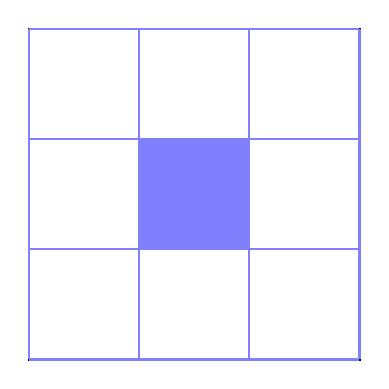
\begin{tikzpicture}[>=stealth,thick,scale=0.7]
			\def\n{1}
			\def\a{3}
			\pgfmathsetmacro{\m}{int(3^(\n))}
			\def\hv#1{
				\ifnum#1>0
				\fill[blue!50] (-\a/3,-\a/3) rectangle (\a/3,\a/3);
				\pgfmathtruncatemacro{\k}{#1-1}
				\foreach \i in {0,...,3}{\begin{scope}[shift={(90*\i:2)},scale=1/3]\hv{\k}\end{scope}}
				\foreach \i in {0,...,3}{\begin{scope}[shift={(45+90*\i:{4/sqrt(2)})},scale=1/3]\hv{\k}\end{scope}}
				\fi
			}
			\draw(-\a,-\a) rectangle (\a,\a);
			\hv{\n}
			\foreach \i in {0,1,...,\m}{
				\draw[blue!50] 
				({-\a+2*\i *\a/\m},\a)--++(270:2*\a)
				(\a,{-\a+2*\i *\a/\m})--++(180:2*\a)
				;
			}
		\end{tikzpicture}
		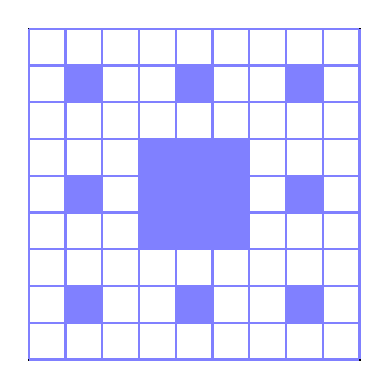
\begin{tikzpicture}[>=stealth,thick,scale=0.7]
			\def\n{2}
			\def\a{3}
			\pgfmathsetmacro{\m}{int(3^(\n))}
			\def\hv#1{
				\ifnum#1>0
				\fill[blue!50] (-\a/3,-\a/3) rectangle (\a/3,\a/3);
				\pgfmathtruncatemacro{\k}{#1-1}
				\foreach \i in {0,...,3}{\begin{scope}[shift={(90*\i:2)},scale=1/3]\hv{\k}\end{scope}}
				\foreach \i in {0,...,3}{\begin{scope}[shift={(45+90*\i:{4/sqrt(2)})},scale=1/3]\hv{\k}\end{scope}}
				\fi
			}
			\draw(-\a,-\a) rectangle (\a,\a);
			\hv{\n}
			\foreach \i in {0,1,...,\m}{
				\draw[blue!50] 
				({-\a+2*\i *\a/\m},\a)--++(270:2*\a)
				(\a,{-\a+2*\i *\a/\m})--++(180:2*\a)
				;
			}
		\end{tikzpicture}
		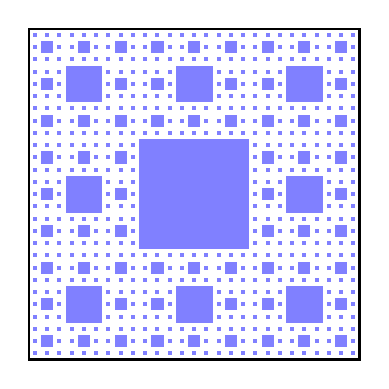
\begin{tikzpicture}[>=stealth,thick,scale=0.7]
			\def\n{4}
			\def\a{3}
			\def\hv#1{
				\ifnum#1>0
				\fill[blue!50] (-\a/3,-\a/3) rectangle (\a/3,\a/3);
				\pgfmathtruncatemacro{\k}{#1-1}
				\foreach \i in {0,...,3}{\begin{scope}[shift={(90*\i:2)},scale=1/3]\hv{\k}\end{scope}}
				\foreach \i in {0,...,3}{\begin{scope}[shift={(45+90*\i:{4/sqrt(2)})},scale=1/3]\hv{\k}\end{scope}}
				\fi
			}
			\draw (-\a,-\a) rectangle (\a,\a);
			\hv{\n}
		\end{tikzpicture}
	\end{center}
	\loigiai{
		Lần phân chia thứ nhất, $1$ hình vuông thành $9$ hình vuông con, diện tích hình vuông tô màu xanh là $u_1=\dfrac{1}{9}$.\\
		Lần phân chia thứ hai, $8$ hình vuông thành $9$ hình vuông con, diện tích hình vuông tô màu xanh tăng thêm là $u_2=\dfrac{1}{9}\left(\dfrac{8}{9}\right)$.\\
		Lần phân chia thứ ba, $8^2$ hình vuông thành $9$ hình vuông con, diện tích hình vuông tô màu xanh tăng thêm là $u_3=\dfrac{1}{9}\left(\dfrac{8}{9}\right)^2$.\\
		Lần phân chia thứ tư, $8^3$ hình vuông thành $9$ hình vuông con, diện tích hình vuông tô màu xanh tăng thêm là $u_4=\dfrac{1}{9}\left(\dfrac{8}{9}\right)^3$.\\
		Lần phân chia thứ năm, $8^4$ hình vuông thành $9$ hình vuông con, diện tích hình vuông tô màu xanh tăng thêm là $u_5=\dfrac{1}{9}\left(\dfrac{8}{9}\right)^4$.\\
		Như vậy diện tích các hình vuông tăng thêm sau mỗi lần chia  tạo thành cấp số nhân có công bội là $q=\dfrac{8}{9}$, số hạng đầu là $u_1=\dfrac{1}{9}$.\\
		Do đó, tổng diện tích hình vuông tô màu xanh sau $5$ lần chia là\\
		\[u_1+u_2+u_3+u_4+u_5=\dfrac{1-q^5}{1-q}\cdot u_1=\dfrac{1-\left(\dfrac{8}{9}\right)^5}{1-\dfrac{8}{9}}\cdot \dfrac{1}{9}=\dfrac{26281}{39366}.\]	
		
	}
\end{vd}

\begin{vd}%[TH] %[DCHT Toán 11 - KNTT - Dung Phuong] %[1K2B7-7]
	Một khay nước có nhiệt độ $23^\circ$ được đặt vào ngăn đá của tủ lạnh. Biết sau mỗi giờ, nhiệt độ của nước giảm $20\%$. Tính nhiệt độ của khay nước đó sau $6$ giờ theo đơn vị độ $C$.
	\dapso{$ \approx 7,5^\circ $ gam}
	\loigiai{
		Nhiệt độ sau mỗi giờ của khay nước theo thứ tự lập thành cấp số nhân với $u_1=23.(1-20\%)$ và $q=(1-20\%)$.\\
		Ta có $u_6=u_1.q^5=23.(1-20\%)^6 \approx 7,5$.\\
		Nhiệt độ của khay nước sau $6$ giờ là $ \approx 6,0^\circ $.
	}
	
\end{vd}
\begin{vd}%[TH] %[DCHT Toán 11 - KNTT - Dung Phuong] %[1K2B7-7]
	Chu kì bán rã của nguyên tố phóng xạ poloni $210$ là $138$ ngày, nghĩa là sau $138$ ngày, khối lượng của nguyên tố đó chi còn một nửa (theo: https://vi.wikipedia.org/wiki/Poloni-210). Tính khối lượng còn lại của $20$ gam poloni $210$ sau:
	\begin{listEX}[2]
		\item [a)]  $690$ ngày;
		\item [b)] $7314$ ngày (khoảng $20$ năm).
	\end{listEX}
	\dapso{$\dfrac{20}{2^{53}}$ gam}
	\loigiai{
		\begin{listEX}[1]
			\item [a)] Ta có $\dfrac{690}{138}=5$ suy ra khối lượng còn lại sau 690 này là $\dfrac{20}{2^5}=0{,}625$ gam;
			\item [b)] Ta có $\dfrac{7314}{138}=53$ suy ra khối lượng còn lại sau 7314 này là $\dfrac{20}{2^{53}}$ gam.
		\end{listEX}
	}
\end{vd}	
\begin{vd}%[TH] %[DCHT Toán 11 - KNTT - Dung Phuong] %[1K2K7-7]
	Tế bào E.Coli trong điều kiện nuôi cấy thích hợp cứ $20$ phút lại phân đôi một lần. Hỏi sau $24$ giờ, tế bào ban đầu sẽ phân chia thành bao nhiếu tế bào?
	\dapso{$2^{72}$}
	\loigiai{
		Lần phân chia thứ nhất, $1$ tế bào thành $2$ tế bào, số tế bào lần $1$ phân chia là $u_1 = 2$.\\
		Lần phân chia thứ hai $2$, số tế bào lần $2$ phân chia là  $u_2=2\cdot 2 = u_1 \cdot 2$.\\
		Lần phân chia thứ $3$ có  $4$ tế bào phân chia, số tế bào lần $3$ phân chia là $u_3=2\cdot u_2$.\\
		Như vậy một tế bào phân đôi sẽ tạo thành cấp số nhân có công bội là $2$, số hạng đầu là $u_1=2$.\\
		Sau $n$ lần phân chia từ một tế bào phân được thành $u_n=2^{n-1}u_1$.\\
		Đổi $24$ giờ $=24 \cdot 60 =  72 \cdot 20$ (phút)  $\Rightarrow 24$ giờ gấp $72$ lần $20$ phút. \\
		Do đó, sau $24$ giờ số tế bào nhận được là $u_{72}=2^{71}\cdot 2 = 2^{72}$ (tế bào).
	}
\end{vd}

\subsubsection{Bài tập tự luận}
 


\begin{bt}%[TH] %[DCHT Toán 11 - KNTT - Dung Phuong] %[1K2B7-7]
	Một quốc gia có dân số năm 2011 là $P$ triệu người. Trong $10$ năm tiếp theo, mỗi năm dân số tăng $a \%$. Chứng minh rằng dân số các năm từ năm 2011 đến năm 2021 của quốc gia đó tạo thành cấp số nhân. Tìm công bội của cấp số nhân này.
	\loigiai{
		Coi ngày điều tra dân số năm 2011 và năm 2021 trùng nhau thì từ năm 2011 đến năm 2021 là 10 năm. Vậy dân số nước ta tính đến năm 2021 là 
		\[u_{10} = P\cdot \left(1+a\%\right)^{10}.\]
		Ta có \[u_{1} = P\cdot \left(1+a\%\right)^{1}.\]
		\[u_{2} = P\cdot \left(1+a\%\right)^{2}.\]
		Và công bội của cáp số nhân này là $\, \dfrac{u_2}{u_1} = q = \dfrac{P\cdot \left(1+a\%\right)^{2}}{P\cdot \left(1+a\%\right)^{1}} = 1+a\%.$
	}
\end{bt}
\begin{bt}%[TH] %[DCHT Toán 11 - KNTT - Dung Phuong] %[1K2B7-7]
	Vào năm 2020, dân số của một quốc gia là khoảng $97$ triệu người và tốc độ tăng trưởng dân số là $0{,}91 \%$. Nếu tốc độ tăng trưởng dân số này được giữ nguyên hằng năm, hãy ước tính dân số của quốc gia đó vào năm 2030.
	\dapso{$106{,}1973784$}
	\loigiai{
		Dân số năm 2021 tăng lên so với năm 2020 là $97 \cdot 0{,}91 \% $ triệu người.\\
		Dân số năm 2021 là 
		\begin{center}
			$97 + 97 \cdot 0{,}91 \% = 97\cdot (1+0{,}91 \%)$ triệu người.
		\end{center}
		Dân số năm 2022 tăng lên so với năm 2021 là $97\cdot (1+0{,}91 \%)\cdot 0{,}91 \% $ triệu người.\\
		Dân số năm 2022 là 
		\begin{center}
			$97\cdot (1+0{,}91 \%) + 97\cdot (1+0{,}91 \%) \cdot 0{,}91 \% = 97\cdot (1+0{,}91 \%)^2$ triệu người.
		\end{center}
		Dân số năm 2023 tăng lên so với năm 2021 là $97\cdot (1+0{,}91 \%)^2\cdot 0{,}91 \% $ triệu người.\\
		Dân số năm 2023 là
		\begin{center}
			$97\cdot (1+0{,}91 \%)^2 + 97\cdot (1+0{,}91 \%)^2\cdot 0{,}91 \% = 97\cdot (1+0{,}91 \%)^3$ triệu người.
		\end{center}
		Tương tự vậy ta có dân số năm 2030 là $97\cdot (1+0{,}91 \%)^{10} = 106{,}1973784$ triệu người.
	}
\end{bt}
\begin{bt}%[TH] %[DCHT Toán 11 - KNTT - Dung Phuong] %[1K2B7-7]
	Một tỉnh có $2$ triệu dân vào năm 2020 với tỉ lệ tăng dân số là $1$ \%/năm. Gọi $u_n$ là số dân của tỉnh đó sau $n$ năm. Giả sử tỉ lệ tăng dân số là không đổi.
	\begin{enumEX}[a)]{1} 
		\item Viết công thức tính số dân của tỉnh đó sau $n$ năm kể từ năm 2020.
		\item Tính số dân của tỉnh đó sau $10$ năm kể từ năm 2020.  
	\end{enumEX}
	\loigiai{
		\begin{enumEX}[a)]{1} 
			\item Với $u_n$ là số dân của tỉnh đó sau $n$ năm. \\
			Ta có $u_1=2 \cdot 1,01$ (triệu dân).\\
			$u_{n+1}=u_n+u_n\cdot 0{,}01 = 1{,}01u_n$. \\
			Do đó, $(u_n)$ là cấp số nhân với số hạng đầu $u_1=2 \cdot 1,01$ và công bội $q=1{,}01$. \\
			Vậy công thức tính số dân của tỉnh đó sau $n$ năm là $u_n=u_1q^{n-1}\Rightarrow u_n=2\cdot 1{,}01^{n}$.
			\item Số dân của tỉnh đó sau $10$ năm kể từ năm 2020 là $u_{10}=2\cdot 1{,}01^10 = 2{,}209$ (triệu dân).
		\end{enumEX}
	}
\end{bt}
\begin{bt}%[TH] %[DCHT Toán 11 - KNTT - Dung Phuong] %[1K2B7-7]
	Giả sử một thành phố có dân số năm 2022 là khoảng $2{,}1$ triệu người và tốc độ gia tăng dân số trung bình mỗi năm là $0{,}75 \%$.
	\begin{listEX}[1]
		\item [a)]  Dự đoán dân số của thành phố đó vào năm $2032$; \dapso{$\approx2262924$ (người)}
		\item [b)]  Nếu tốc độ gia tăng dân số vẫn giữ nguyên như trên thì uớc tính vào năm nào dân số của thành phố đó sẽ tăng gấp đôi so với năm $2022$?  \dapso{$2116$}	\end{listEX}
	
	\loigiai{
		\begin{listEX}
			\item [a)] 	Giả sử dân số năm $2022$ là $u_1=2{,}1\cdot 10^6$ thì dân số năm 
			$2023$ 
			là 
			$u_2=u_1+ 0{,}0075u_1=1{,}0075u_1$.\\
			Tương tự dân số năm $2024$ là $u_3=1{,}0075u_2$.\\
			Do đó dân số của thành phố qua các năm lập thành một cấp số nhân với 
			$u_1=2{,}1\cdot10^6$; $q=1{,}0075$.\\
			Vậy dân số năm $2032$ tương ứng với $u_{11}=u_1\cdot q^{10}=2,1\cdot 
			10^6\cdot1{,}0075^{10}\approx2262924$ (người).
			\item [b)] Giả sử đến năm thứ $n$ thì dân số gấp đôi năm $2022$. \\
			Suy ra 
			$u_n=2u_1 \Leftrightarrow q^{n-1}=2\Leftrightarrow  1{,}0075^{n-1}=2 
			\Leftrightarrow n \approx 93{,}7.$\\
			Vậy $94$ năm sau tức là năm $2116$ thì dân số thành phố sẽ gấp đôi năm $2022$.
	\end{listEX}}
\end{bt}
\begin{bt}%[TH] %[DCHT Toán 11 - KNTT - Dung Phuong] %[1K2B7-7]
	Giả sử anh Tuấn kí hợp đồng lao động trong $10$ năm với điều khoản về tiền lương như sau: Năm thứ nhất, tiền lương của anh Tuấn là $60$ triệu. Kể từ năm thứ hai trở đi, mỗi năm tiền lương của anh Tuấn được tăng lên $8 \%$. Tính tổng số tiền lương anh Tuấn lĩnh được trong $10$ năm đi làm (đơn vị: triệu đồng, làm tròn đến hàng phần nghìn).
	\dapso{$\approx 869{,}194$ triệu người}
	\loigiai{
		Gọi $u_n$ là số tiền lương (triệu đồng) anh Tuấn được lĩnh ở năm làm việc thứ $n$. Ta có: $u_1=60$;
		\[u_n=u_{n-1}+u_{n-1} \cdot 0{,}08=u_{n-1} \cdot(1+0{,}08)=u_{n-1} \cdot 1{,}08. \]
		Do đó, $\left(u_n\right)$ là cấp số nhân có số hạng đầu $u_1=60$, công bội $q=1{,}08$. Áp dụng công thức tính tổng $S_n$, ta có tổng số tiền lương anh Tuấn lĩnh được trong $10$ năm đi làm là
		\[S_{10}=\dfrac{60\cdot\left(1-1{,}08^{10}\right)}{1-1{,}08} \approx 869{,}194\ (\text{triệu người}). \]
	}
\end{bt}
\begin{bt}%[TH] %[DCHT Toán 11 - KNTT - Dung Phuong] %[1K2B7-7]
	Một công ty xây dựng mua một chiếc máy ủi với giá $3$ tỉ đồng. Cứ sau mỗi năm sử dụng, giá trị của chiếc máy ủi này lại giảm $20 \%$ so với giá trị của nó trong năm liền trước đó. Tìm giá trị còn lại của chiếc máy ủi đó sau $5$ năm sử dụng.
	\dapso{$983$ triệu đồng}
	\loigiai{
		Gọi $u_n$ là Giá trị của máy ủi sau $n$ sử dụng. \\
		Dãy số ($u_n$) là một cấp số nhân có $u_1=3.0,8$, $q=0{,}8$.\\
		Số hạng tổng quát của cấp số nhân này là $u_n=3\cdot 0{,}2^{n}$.\\
		Ta có $u_5=3\cdot 0{,}8^5=0{,}98304$.\\
		Tương ứng giá trị của chiếc máy ủi sau $5$ năm xấp xỉ $983$ triệu đồng.
	}
\end{bt}
\begin{bt}%[TH] %[DCHT Toán 11 - KNTT - Dung Phuong] %[1K2B7-7]
	Một gia đình mua một chiếc ô tô giá $800$ triệu đồng. Trung bình sau mỗi năm sử dụng, giá trị còn lại của ô tô giảm đi $4 \%$ (so với năm trước đó).
	\begin{enumEX}[a)]{1} 
		\item Viết công thức tính giá trị của ô tô sau $1$ năm, $2$ năm sử dụng.
		\item Viết công thức tính giá trị của ô tô sau $n$ năm sử dụng.
		\item Sau $10$ năm, giá trị của ô tô ước tính còn bao nhiêu triệu đồng? 
	\end{enumEX} 
	\dapso{$\approx 531{,}87$ triệu đồng}
	\loigiai{
		Gọi $u_n$ là giá trị còn lại của ô tô sau $n$ năm sử dụng. 
		\begin{enumEX}[a)]{1} 
			\item Giá trị của ô tô sau $1$ năm sử dụng là $u_1=800-800\cdot0{,}04=800\cdot0{,}96=768$ triệu đồng.\\
			Giá trị của ô tô sau $2$ năm sử dụng là $u_2=u_1-u_1\cdot0{,}04=u_1\cdot0{,}96=737{,}28$ triệu đồng.
			\item Ta có $u_n=u_{n-1}-u_{n-1}\cdot0{,}04=u_{n-1}\cdot0{,}96$. \\
			Do đó, $(u_n)$ là cấp số nhân với số hạng đầu $u_1=768$ và công bội $q=0{,}96$. \\
			Vậy sau $n$ năm sử dụng, giá trị còn lại của chiếc ô tô là $u_n=u_1q^{n-1}\Rightarrow u_n=768\cdot0{,}96^{n-1}$.
			\item Sau $10$ năm, ước tính giá trị của ô tô còn lại là $u_{10}=768\cdot0{,}96^9\approx 531{,}87$ triệu đồng.
		\end{enumEX} 
	}
\end{bt}
% \begin{bt} [VD] %[DCHT Toán 11 - KNTT - Dung Phuong] %[1K2K7-7]
% 	Ông An vay ngân hàng $1$ tỉ đồng với lãi suất $12\%/$năm. Ông đã trả nợ theo cách: Bắt đầu từ tháng thứ nhất sau khi vay, cuối tháng ông trả ngân hàng số tiền là $a$ (đồng) và đã trả hết nợ sau đúng $2$ năm kể từ ngày vay. Hỏi số tiền mỗi tháng mà ông An phải trả là bao nhiêu đồng (làm tròn kết quả đến hàng nghìn)?
% 	\dapso{$47073500$}
% 	\loigiai{
% 		Do lãi suất là $12\%$/năm tương đương với lãi là $1\%$/tháng.\\
% 		Sau $1$ tháng, ông An còn nợ là: $10^9.(1+1\%)-a=10^9.(1,01)-S_1$.\\
% 		Sau $2$ tháng, ông An còn nợ là: $10^9.(1.01)^2-a.(1.01)-a=10^9(1,01)^2-S_2$.\\
% 		Sau $3$ tháng, ông An còn nợ là: $10^9.(1.01)^3-a(1.01)^2-a(1.01)-a=10^9.(1.01)^3-S_3$.\\
% 		Sau $24$ tháng, ông An còn nợ là: $10^9.(1.01)^{24}-S_{24}=0$.\\
% 		Do đó $S_{24}=10^9.(1.01)^{24}  \Leftrightarrow a.\dfrac{1-(1.01)^{24}}{1-(1.01)}=10^9.(1.01)^{24} \Leftrightarrow a =\dfrac{10^9.(1.01)^{24}.0.01}{(1.01)^{24}-1}\approx 47073472,22$.\\
% 		Vậy mỗi tháng ông An phải trả $47073500$.
% 	}
% \end{bt}
\begin{bt}%[VD] %[DCHT Toán 11 - KNTT - Dung Phuong] %[1K2K7-7]
	\immini
	{
		Một người nhảy bungee (một trò chơi mạo hiểm mà người chơi nhảy từ một nơi có địa thế cao xuống với dây đai an toàn buộc xung quanh người) từ một cây cầu và căng một sợi dây dài $100$ m. Sau mỗi lần rơi xuống, nhờ sự đàn hồi của dây, người nhảy được kéo lên một quãng đường có độ dài bằng $75$\% so với lần rơi trước đó và lại bị rơi xuống đúng bằng quãng đường vừa được kéo lên. Tính tổng quãng đường người đó đi được sau $10$ lần kéo lên và lại rơi xuống. 
	}
	{
		\begin{tikzpicture}[xscale=.5, font=\small, line join=round, line cap=round, >=stealth,yscale=1]
			\def\a{-0.12} % Hệ số a phải khác 0
			\def\b{0.86}
			\def\c{0}
			\def\m{-0.12} % Hệ số a phải khác 0
			\def\n{0.86}
			\def\p{-0.3}
			\clip (-2,-2)rectangle(9,2);
			\fill[red!40] (-2,1.8)--(9,1.8)--(9,1.55)--(-2,1.55)--cycle;%Mặt phẳng của cây cầu
			\fill[green!50] (-2,1.55)--(0,0)--(1.5,-1)--(-1,-2)--(-2,-2)--cycle;
			\fill[green!50] (9,1.55)--(7,0)--(5.5,-1)--(8,-2)--(9,-2)--cycle;
			\fill[blue!40] (-1,-2)--(8,-2)--(5.5,-1)--(1.5,-1)--cycle;
			\draw[color=blue!50,line width=2pt,<->] (2,-.5)--(2,1.5)node[left,midway]{$100$ m};	
			\draw[color=blue!50,line width=2pt,<->] (5,-.5)--(5,1)node[midway,right]{$0{,}75\cdot100$ m};
			\draw(3.5,1.55)--(3.5,-.25)node[rotate=200]{\faChild};
			\draw[color=white,<->] (3.5,1.8)--(3.5,1.55); 
		\end{tikzpicture}
	}
	\dapso{$\approx666{,}2 \text{ m}$}
	\loigiai{
		Gọi $u_n$ là quãng đường người đó được kéo lên ở lần thứ $n$ được kéo lên và lại rơi xuống (đơn vị tính: mét). \\
		Ta có $u_1=0{,}75\cdot100=100\cdot1{,}5=75$ m và $u_n=0{,}75\cdot u_{n-1}$. \\
		Vậy $(u_n)$ là cấp số nhân với số hạng đầu $u_1=75$ và công bội $q=0{,}75$. \\
		Tổng quãng đường người đó đi được sau $10$ lần kéo lên và lại rơi xuống là 
		$$\begin{aligned}
			S&=100+2u_1+2u_2+\cdots+2u_{10}\\
			&=100+2S_{10}
			=100+2\cdot\dfrac{75\left(1-0{,}75^{10}\right)}{1-0{,}75}\\
			&\approx666{,}2 \text{ m}.
		\end{aligned}$$ 
	}
\end{bt}
\begin{bt} [TH] %[DCHT Toán 11 - KNTT - Dung Phuong] %[1K2B7-7]
	Một cái tháp có $11$ tầng. Diện tích của mặt sàn tầng $2$ bằng nửa diện tích của mặt đáy tháp và diện tích của mặt sàn mỗi tầng bằng nửa diện tích của mặt sàn mỗi tầng ngay bên dưới. Biết mặt đáy tháp có diện tích là $12 288m^2$. Tính diện tích của mặt sàn tầng trên cùng của tháp theo đơn vị mét vuông.
	\dapso{$12m^2$}
	\loigiai{ (Lưu ý: Một số nơi xem tầng 1 là tầng trệt. Nên bài toán này giống bài toán tháp 10 tầng ở phần trên)
		Do diện tích của mặt sàn tính từ tầng một lập thành một cấp số nhân với $u_2=\dfrac{1}{2}.12288=6144$ và $q=\dfrac{1}{2}$.\\
		Ta có $\heva{u_2&=6144 \\ q&=\dfrac{1}{2}}  \Leftrightarrow \heva{u_1&=12288 \\ q&=\dfrac{1}{2}}$.\\
		Ta có $u_{11}=u_1.q^{10}=12288.\dfrac{1}{2^{10}}=12m^2$.
		Vậy diện tích của mặt sàn tầng trên cùng là	$12m^2$.
	}
\end{bt}

\begin{bt}%[TH]%[DCHT Toán 11 - KNTT - Dung Phuong]%[1K2B7-7]
	\immini{Cho hình vuông $C_1$ có cạnh bằng $4$. Người ta chia mỗi cạnh hình vuông thành bốn phần bằng nhau và nối các điểm chia một cách thích hợp để có hình vuông $C_2$ . Từ hình vuông $C_2$ lại làm tiếp tục như trên để có hình vuông $C_3$. Cứ tiếp tục quá trình như trên, ta nhận được dãy các hình vuông $C_1, C_2, C_3, \ldots , C_n, \ldots$ Gọi $a_n$ là độ dài cạnh hình vuông $C_n$. Chứng minh rằng dãy số $\left(a_n\right)$ là cấp số nhân.}{
		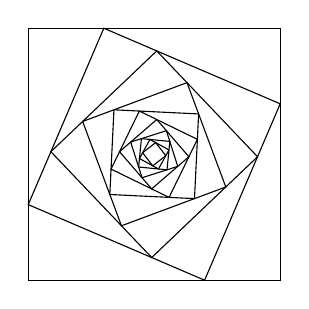
\begin{tikzpicture}[scale=.8]
			\def\a{2}  %cạnh hình vuông
			\def\t{.7}  % tỷ lệ điểm cho vòng lặp tiếp
			\path 
			(-\a,-\a) coordinate (A1)
			(-\a,\a) coordinate (B1)
			(\a,\a) coordinate (C1)
			(\a,-\a) coordinate (D1);
			\draw (A1)--(B1)--(C1)--(D1)--cycle;
			\foreach \i[count=\j from 2] in {1,...,10}
			\draw
			(barycentric cs:A\i=\t,B\i=1-\t) coordinate (A\j)--
			(barycentric cs:B\i=\t,C\i=1-\t) coordinate (B\j)--
			(barycentric cs:C\i=\t,D\i=1-\t) coordinate (C\j)--
			(barycentric cs:D\i=\t,A\i=1-\t) coordinate (D\j)--cycle
			;	
			% \node at (0,-2.2) [below]{\textit{Hình 4}};
		\end{tikzpicture}	
	}
	\loigiai{
		\immini{Gọi cạnh một hình vuông thứ $n$, $n+1$ lần lượt là $a_n, a_{n+1}$.\\
			Do $MN=\sqrt{MB^2+BN^2}=\sqrt{\left(\dfrac{AB}{4}\right)^2+\left(\dfrac{3AB}{4}\right)^2 }=AB\cdot\dfrac{\sqrt{10}}{4}$.\\
			Nên ta có cạnh hình vuông thứ $n+1$ là:\\ $a_{n+1}=a_n.\dfrac{\sqrt{10}}{4}$.\\
			Vậy dãy số $\left(a_n\right)$ là cấp số nhân.	
		}{
			\begin{tikzpicture}[scale=0.8,>=stealth, font=\footnotesize, line join=round, line cap=round]
				\path
				(0,0) coordinate (A)
				(4,0) coordinate (B)
				(4,4) coordinate (C)
				(0,4) coordinate (D)
				($(A)!0.75!(B)$) coordinate (M)
				($(B)!0.75!(C)$) coordinate (N)
				($(C)!0.75!(D)$) coordinate (P)
				($(D)!0.75!(A)$) coordinate (Q)
				;
				\draw (A)--(B)--(C)--(D)--cycle (M)--(N)--(P)--(Q)--cycle;
				\node at ($(A)!0.5!(B)$)[below]{$a_n$};
				\node at ($(M)!0.5!(N)$)[left]{$a_{n+1}$};
				\foreach \p/\q in {A/180,B/0,C/0,D/180,M/-90,N/0,P/90,Q/180}
				\fill[black] (\p) circle (1.0pt) ($(\p)+(\q:2.5mm)$) node{$\p$};
		\end{tikzpicture}
	}
	}
\end{bt}

\begin{bt}%[TH] %[DCHT Toán 11 - KNTT - Dung Phuong] %[1K2B7-7]
	Một cây đàn organ có tần số âm thanh các phím liên tiếp tạo thành một cấp số nhân. Cho biết tần số phím La trung là $400$ Hz và tần số của phím La cao cao hơn $12$ phím là $800$ Hz (nguồn: https://vi.wikipedia.org/wikiOrgan). Tìm công bội của cấp số nhân nói trên (làm tròn kết quả đến hàng phần nghìn).
	\dapso{$q = \pm \sqrt[12]{2}$}
	\loigiai{
		Theo đề ta có $\heva{&u_1=400\\&u_{13}=800} \Leftrightarrow \heva{&u_1=400\\&u_1q^{12}=800} \Rightarrow q^{12} = 2 \Rightarrow q = \pm \sqrt[12]{2}$.
	}
\end{bt}


\begin{bt}%[VD]%[DCHT Toán 11 - KNTT - Dung Phuong] %[1K2K7-7] 
	Một loại thuốc được dùng mỗi ngày một lần. Lúc đầu nồng độ thuốc trong máu của bệnh nhân tăng nhanh, nhưng mỗi liều kế tiếp có tác dụng ít hơn liều trước đó. Lượng thuốc trong máu ở ngày thứ nhất là $50 \,\mathrm{mg}$, và mỗi ngày sau đó giảm chỉ còn một nửa so với ngày kề trước đó. Tính tổng lượng thuốc (tính bằng $\mathrm{mg}$) trong máu của bệnh nhân sau khi dùng thuốc $10$ ngày liên tiếp.
	\dapso{$99{,}902$ mg.}
	\loigiai{
		Gọi $u_n$ là giá trị của lượng thuốc trong máu của bệnh nhân trong ngày thứ $n$. \\
		Dãy số này là một cấp số nhân có $u_1=50$, $q=\dfrac{1}{2}$.\\
		Tổng của $n$ số hạng đầu tiên của cấp số nhân là $S_n=u_1\dfrac{1-q^n}{1-q}$.\\
		Theo bài toán, ta có $S_{10}=50 \cdot\dfrac{1-\left(\dfrac{1}{2}\right)^{10}}{1-\dfrac{1}{2}} \approx 99{,}902$.\\
		Vậy tổng lượng thuốc trong máu của bệnh nhân sau khi dùng thuốc $10$ ngày liên tiếp là $99{,}902$ mg.	
	}
\end{bt}
\subsubsection{Câu hỏi trắc nghiệm}
\Opensolutionfile{ans}[ans/ans-1K2-2-Dang7]
\begin{ex}%[1K2K7-7]
	\immini{
		Cho hình vuông có cạnh là $1$. Nối các trung điểm của hình vuông trên ta được một hình vuông có diện tích $S_1$, tiếp tục quá trình trên với các hình vuông với diện tích là $S_2$; $S_3$; $\ldots ;S_n;\ldots$. Tính tổng vô hạn $S_1+ S_2+ S_3+\cdots+S_n+\cdots$.
		\choice
		{$2$}
		{$\dfrac{1}{2}$}
		{\True $1$}
		{$\dfrac{3}{2}$}
	}
	{\hspace*{1 cm}
		\begin{tikzpicture}[scale=0.8,line cap=round,line join=round]
			\path
			(0,0) coordinate (A)
			(4,0) coordinate (B)
			(0,4) coordinate (D);			
			\coordinate (C) at ($(B)-(A)+(D)$);
			\coordinate (H) at ($(A)!0.5!(B)$);
			\coordinate (I) at ($(A)!0.5!(D)$);
			\coordinate (J) at ($(D)!0.5!(C)$);
			\coordinate (K) at ($(B)!0.5!(C)$);
			\coordinate (E) at ($(I)!0.5!(H)$);
			\coordinate (F) at ($(H)!0.5!(K)$);
			\coordinate (G) at ($(K)!0.5!(J)$);
			\coordinate (O) at ($(J)!0.5!(I)$);
			\coordinate (M) at ($(E)!0.5!(F)$);
			\coordinate (N) at ($(F)!0.5!(G)$);
			\coordinate (P) at ($(G)!0.5!(O)$);
			\coordinate (Q) at ($(O)!0.5!(E)$);
			\draw (A)--(B)--(C)--(D)--cycle (I)--(H)--(K)--(J)--cycle
			(E)--(F)--(G)--(O)--cycle (M)--(N)--(P)--(Q)--cycle;
			\foreach \p in {A,B,C,D,E,F,G,H,I,J,K,M,N,P,Q,O}
			\fill[black] (\p) circle (1.0pt);			
		\end{tikzpicture}
	}
	\loigiai{
		Ta có $S_1=\dfrac{1}{2}$, $S_2=\dfrac{1}{4}$, $S_3=\dfrac{1}{8},\cdots  S_n=\dfrac{1}{2^n},\ldots$ tạo thành $1$ cấp số nhân với công bội $q=\dfrac{1}{2}<1$. \\
		Vậy $S_1+ S_2+ S_3+\cdots+S_n+\cdots=\dfrac{\dfrac{1}{2}}{1-\dfrac{1}{2}}=1$.
	}
\end{ex}
\begin{ex}%[1K2K7-7]
	Cho $n$ là số nguyên dương và $n$ tam giác $A_1B_1C_1,A_2B_2C_2,\ldots,A_nB_nC_n$, trong đó các điểm lần ${A}_{i+1},{B}_{i+1},{C}_{i+1}$ lượt nằm trên các cạnh $B_iC_i,A_iC_i,A_iB_i(i=1,2,\ldots,n-1)$ sao cho ${A}_{i+1}C_i=3{A}_{i+1}B_i,{B}_{i+1}A_i=3{B}_{i+1}C_i,{C}_{i+1}B_i=3{C}_{i+1}A_i$. Gọi $S$ là tổng tất cả các diện tích của tam giác $A_1B_1C_1,A_2B_2C_2,\ldots,A_nB_nC_n$ biết rằng tam giác $A_1B_1C_1$ có diện tích bằng $\dfrac{9}{16}$. Tìm số nguyên dương sao cho $S=\dfrac{{16}^{29}-7^{29}}{{16}^{29}}$.
	\choice
	{$n=28$}
	{$n=2018$}
	{$n=30$}
	{\True $n=29$}
	\loigiai{
		Gọi $S_i(i=1,2,3,...,n)$ là diện tích của $\Delta A_iB_iC_i$. Ta có $\dfrac{S_{A_1B_2C_2}}{S_{A_1B_1C_1}}=\dfrac{A_1B_2}{A_1C_1}\cdot \dfrac{A_1C_2}{A_1B_1}=\dfrac{1}{4}\cdot \dfrac{3}{4}=\dfrac{3}{16}$. Tương tự, ta có $\dfrac{S_{A_2B_1C_2}}{S_{A_1B_1C_1}}=\dfrac{S_{A_2B_2C_1}}{S_{A_1B_1C_1}}=\dfrac{3}{16}$. Do đó $\dfrac{S_{A_2B_2C_2}}{S_{A_1B_1C_1}}=1-3\cdot \dfrac{3}{16}=\dfrac{7}{16}\Rightarrow S_2=\dfrac{7}{16}S_1$.\\
		Tương tự, ta có ${S}_{i+1}=\dfrac{7}{16}S_i,i=1,2,\ldots,n$.
		Khi đó $$S=S_1\left[1+\dfrac{7}{16}+\cdots+{\left(\dfrac{7}{16}\right)}^{n-1}\right]=\dfrac{9}{16}\cdot \dfrac{1-{\left(\dfrac{7}{16}\right)}^n}{1-\dfrac{7}{16}}=1-{\left(\dfrac{7}{16}\right)}^n.$$
		Theo giả thiết ta có $1-{\left(\dfrac{7}{16}\right)}^n=1-{\left(\dfrac{7}{16}\right)}^{29}\Leftrightarrow n=29$.}
\end{ex}
\begin{ex}%[1K2K7-7]
	Người ta thiết kế một cái tháp gồm $11$ tầng. Diện tích bề mặt trên của mỗi tầng bằng nửa diện của mặt trên tầng ngay bên dưới và diện tích tầng $1$ bằng nửa diện tích của đế tháp. Biết đế tháp có diện tích là $12288\, \mathrm{m}^2$. Tính diện tích mặt trên cùng.
	\choice
	{$12\, \mathrm{m}^2$}
	{\True $6\, \mathrm{m}^2$}
	{$10\, \mathrm{m}^2$}
	{$8\, \mathrm{m}^2$}
	\loigiai{
		Gọi $S_{i}$ là diện tích của tầng thứ $i$ với $i = 1,2,\ldots,11$.\\
		Do giả thiết suy ra $S_{i + 1} = \dfrac{1}{2}S_{i}$ với $i = 1,2,\ldots,10$.\\
		Do đó $\left\{S_{i}\right\}$ là một cấp số nhân với công bội $q = \dfrac{1}{2}$. Do đó  $S_{11} = \dfrac{1}{2^{10}}S_{1} = \dfrac{1}{2^{11}}\cdot 12288 = 6\left(\mathrm{m}^2\right)$.
	}
\end{ex}

\begin{ex}%[1K2K7-7]
	Cho tứ giác $ABCD$ có bốn góc tạo thành cấp số nhân có công bội $ q=2 $. Góc có số đo nhỏ nhất trong bốn góc đó là
	\choice
	{\True $ 24^\circ $}
	{$ 1^\circ $}
	{$ 12^\circ $}
	{$ 30^\circ $}
	\loigiai{
		Gọi số đo bốn góc của tứ giác $ ABCD $ là $ x $, $ 2x $, $ 4x $, $ 8x $.
		\\ Có $ x+2x+4x+8x=360 \Leftrightarrow 15x=360 \Leftrightarrow x=24 $.}
\end{ex}

\begin{ex}%[1K2K7-7]
	Một du khách vào chuồng đua ngựa đặt cược, lần đầu tiên đặt $20000$ đồng, mỗi lần sau tiền đặt gấp đôi lần tiền đặt cược trước. Người đó thua lần $9$ liên tiếp và thắng ở lần thứ $10$. Hỏi du khách đó thắng hay thua bao nhiêu tiền?
	\choice
	{\True Thắng $20000$ đồng}
	{Thua $40000$ đồng}
	{Hòa vốn}
	{Thua $20000$ đồng}
	\loigiai{
		Số tiền đặt cược lần thứ $n$ là $u_n=u_1\cdot 2^{n-1}$ với $u_1=20000$. \\
		Ta có: $u_{10}-\displaystyle\sum_{n=1}^9 u_1\cdot 2^{n-1}=20000\cdot 2^9-\displaystyle\sum_{n=1}^9 20000\cdot 2^{n-1}=20000$. \\
		Vậy du khách thắng $20000$ đồng.
	}
\end{ex}

% \begin{ex}%[1K2K7-7]
% 	Một người gửi tiết kiệm vào ngân hàng với lãi suất $7{,}5$ \%/năm. Biết rằng nếu không rút tiền ra khỏi ngân hàng thì cứ sau mỗi năm số tiền lãi sẽ được nhập vào vốn để tính lãi cho năm tiếp theo. Hỏi sau ít nhất bao nhiêu năm người đó thu được (cả số tiền gửi ban đầu và lãi) gấp đôi số tiền đã gửi, giả định trong khoảng thời gian này lãi suất không thay đổi và người đó không rút tiền ra?
% 	\choice
% 	{$12$ năm}
% 	{$11$ năm}
% 	{\True $10$ năm}
% 	{$9$ năm}
% 	\loigiai{
% 		Áp dụng công thức: $S_n=A(1+r)^n \Rightarrow n=\log_{(1+r)}\left(\dfrac{S_n}{A}\right) \Rightarrow n=\log_{\left(1+7{,}5\%\right)}(2)\approx 9{,}6$.}
% \end{ex}

\begin{ex}%[1K2K7-7]
	Cho tam giác $ ABC $ cân tại $ A $ có cạnh đáy $ BC $,  đường cao $ AH $ và cạnh bên $ AB $ theo thứ tự đó lập thành cấp số nhân công bội $ q $. Giá trị của $ q $ là
	\choice
	{$ q=\dfrac{1}{2}\sqrt{\sqrt{2}+1} $ }
	{$ q=\sqrt{2}+1 $ }
	{$ q=\sqrt{2(\sqrt{2}+1)} $}
	{\True $ q=\dfrac{1}{2}\sqrt{2(\sqrt{2}+1)} $ }
	\loigiai{
		Giả sử $ BC=u_1 $, $ AH=u_1\cdot q $ và $ AB=u_1\cdot q^2 $ với $ u_1> 0, q> 0 $.\\
		Do $ \triangle ABC $ cân tại $ A $ suy ra
		\begin{align*}
			AB^2=AH^2+\dfrac{BC^2}{4}\Leftrightarrow
			& u_1^2\cdot q^4=\dfrac{u_1^2}{4}+u_1^2\cdot q^2\\
			\Leftrightarrow & 4q^4-4q^2-1=0\\
			\Leftrightarrow & q^2=\dfrac{1\pm \sqrt{2}}{2}.
		\end{align*}
		Kết hợp với điều kiện bài toán ta có $ q=\sqrt{\dfrac{1+ \sqrt{2}}{2}}=\dfrac{1}{2}\sqrt{2(\sqrt{2}+1)} $.
	}
\end{ex}
\begin{ex}%[1K2K7-7]
	Giả sử một người đi làm được lĩnh lương khởi điểm là $2.000.000$ đồng/tháng. Cứ $3$ năm người ấy lại được tăng lương một lần với mức tăng bằng $7\%$ của tháng trước đó. Hỏi sau $36$ năm làm việc người ấy lĩnh được tất cả bao nhiêu tiền?
	\choice
	{\True $ 1.287.968.492 $ đồng}
	{$ 10.721.769.110 $ đồng}
	{$ 7{,}068289036\cdot 10^8 $ đồng}
	{$ 429.322.830{,}5 $ đồng}
	\loigiai{
		Ta có $36$ năm tương ứng với $12$ kỳ lương; mỗi kỳ lương có $36$ tháng và kỳ sau tăng $7\%$ so với kỳ trước. Do đó tổng số tiền mỗi kỳ lương là một cấp số nhân với $u_1=36\times 2=72$ (triệu đồng) và công bội $q=1{,}07$.\\
		Vậy tổng số tiền sau $36$ năm là $T=\dfrac{72\cdot \left[(1{,}07)^{12}-1\right]}{1{,}07-1}=1287{,}968492$ (triệu đồng).
	}
\end{ex}

\begin{ex}%[1K2K7-7]
	Từ độ cao $55{,}8$ (mét) của tháp nghiên Pisa nước Italia người ta thả một quả bóng cao su chạm xuống đất. Giả sử mỗi lần chạm đất bóng lại nảy lên độ cao bằng $\dfrac{1}{10}$ độ cao mà bóng đạt trước đó. Tổng độ dài hành trình (mét) của bóng được thả từ lúc ban đầu cho đến khi nó nằm yên trên mặt đất thuộc khoảng nào trong các khoảng sau đây?
	\choice
	{$(69;72)$}
	{$(60;63)$}
	{\True $(67;69)$}
	{$(64;66)$}
	\loigiai{
		Đặt $u_1=55{,}8$ (mét) là quãng đường bóng rơi khi thả xuống, $u_{n+1}=\dfrac{1}{10^{n}} u_1, n\ge 1$ là quãng đường bóng rơi sau lần nảy lên thứ $n$. \\
		Ta có $(u_n)$ là dãy cấp số nhân với $u_1=55{,}8$ và công bội $q=\dfrac{1}{10}$.\\
		Suy ra tổng quãng đường quả bóng rơi xuống là $\displaystyle \lim \limits_{n \rightarrow +\infty} u_1 \cdot \dfrac{1-q^n}{1-q}=\displaystyle \lim \limits_{n \rightarrow +\infty}55{,}8\cdot\dfrac{1-\left( \dfrac{1}{10}\right)^n}{1-\dfrac{1}{10}}=62 $.\\
		Ngoài ra ta còn phải tính tổng quãng đường mà bóng nảy lên. Ta có tổng quãng đường bóng nảy lên bằng tổng quãng đường rơi của bóng trừ đi quãng đường thả rơi xuống.\\
		Vậy tổng quãng đường hành trình của quả bóng là $62+62-55{,}8=68{,}2$ (mét).
	}
\end{ex}

\begin{ex}%[1K2K7-7]
	Một gia đình lập kế hoạch tiết kiệm như sau: Họ lập một sổ tiết kiệm tại một ngân hàng và cứ đầu mỗi tháng họ gửi
	vào sổ tiết kiệm đó $15$ triệu đồng. Giả sử lãi suất tiền gửi không đổi là $0{,}6$ \%/tháng và tiền gửi được tính lãi theo hình thức lãi
	kép. Hỏi sau $3$ năm gia đình đó tiết kiệm được số tiền gần nhất với con số nào dười đây?
	\choice
	{$543240000$ đồng}
	{$589269000$ đồng}
	{$669763000$ đồng}
	{\True $604359000$ đồng}
	\loigiai{
		Gọi $S_0$ triệu đồng là số tiền gia đình đó định kỳ gửi tiết kiệm vào đầu hằng tháng, $r$ là lãi suất tiền gửi hằng tháng. Ta có $S_0=15$ triệu đồng, $r=0{,}6$
		\%/tháng.\\
		Gọi $S_i$, $i=\overline{1,n}$ là số tiền trong sổ tiết kiệm cuối tháng thứ $i$.\\
		Ta có \begin{itemize}
			\item $S_1=S_0+S_0\cdot r=S_0(1+r)$,
			\item  $S_2=\left[ S_0+S_0(1+r)\right]+\left[ S_0+S_0(1+r)\right]r=S_0 (1+r)+S_0(1+r)^2$,
			\item  $\begin{aligned}[t]
				S_3=&\ \left[S_0+S_0(1+r)+S_0(1+r)^2 \right] +\left[S_0+S_0(1+r)+S_0(1+r)^2 \right]r\\
				=&\ S_0(1+r)+S_0(1+r)^2+S_0(1+r)^3,\end{aligned}$,
			\item \ldots
			\item$\begin{aligned}[t]S_n=&\ S_0(1+r)+S_0(1+r)^2+S_0(1+r)^3+\cdots +S_0(1+r)^n\\=&\ S_0\left[ (1+r)+(1+r)^2+(1+r)^3+\cdots+(1+r)^n\right]\\
				=&\  S_0(1+r)\cdot \dfrac{(1+r)^{n}-1}{(1+r)-1}=S_0(1+r)\cdot \dfrac{(1+r)^{n}-1}{r}.
			\end{aligned}$
		\end{itemize}
		Vậy sau $3$ năm, tức cuối tháng thứ $36$ thì gia đình tiết kiệm được số tiền là
		\[S_{36}=15\cdot 10^6(1+0{,}6\cdot 10^{-2})\cdot \dfrac{(1+0{,}6\cdot 10^{-2})^{36}-1}{0{,}6\cdot 10^{-2}}=604358538{,}2 \ \text{đồng}.\]
	}
\end{ex}
\Closesolutionfile{ans}
% \begin{indapan}{10}
% 	{ans/ans-1K2-2-Dang7}
% \end{indapan}
